\PassOptionsToPackage{unicode=true}{hyperref} % options for packages loaded elsewhere
\PassOptionsToPackage{hyphens}{url}
%
\documentclass[]{book}
\usepackage{lmodern}
\usepackage{amssymb,amsmath}
\usepackage{ifxetex,ifluatex}
\usepackage{fixltx2e} % provides \textsubscript
\ifnum 0\ifxetex 1\fi\ifluatex 1\fi=0 % if pdftex
  \usepackage[T1]{fontenc}
  \usepackage[utf8]{inputenc}
  \usepackage{textcomp} % provides euro and other symbols
\else % if luatex or xelatex
  \usepackage{unicode-math}
  \defaultfontfeatures{Ligatures=TeX,Scale=MatchLowercase}
\fi
% use upquote if available, for straight quotes in verbatim environments
\IfFileExists{upquote.sty}{\usepackage{upquote}}{}
% use microtype if available
\IfFileExists{microtype.sty}{%
\usepackage[]{microtype}
\UseMicrotypeSet[protrusion]{basicmath} % disable protrusion for tt fonts
}{}
\IfFileExists{parskip.sty}{%
\usepackage{parskip}
}{% else
\setlength{\parindent}{0pt}
\setlength{\parskip}{6pt plus 2pt minus 1pt}
}
\usepackage{hyperref}
\hypersetup{
            pdftitle={Introducción al Aprendizaje Supervisado},
            pdfauthor={Harold A. Hernández-Roig (hahernan@est-econ.uc3m.es)},
            pdfborder={0 0 0},
            breaklinks=true}
\urlstyle{same}  % don't use monospace font for urls
\usepackage{color}
\usepackage{fancyvrb}
\newcommand{\VerbBar}{|}
\newcommand{\VERB}{\Verb[commandchars=\\\{\}]}
\DefineVerbatimEnvironment{Highlighting}{Verbatim}{commandchars=\\\{\}}
% Add ',fontsize=\small' for more characters per line
\usepackage{framed}
\definecolor{shadecolor}{RGB}{248,248,248}
\newenvironment{Shaded}{\begin{snugshade}}{\end{snugshade}}
\newcommand{\AlertTok}[1]{\textcolor[rgb]{0.94,0.16,0.16}{#1}}
\newcommand{\AnnotationTok}[1]{\textcolor[rgb]{0.56,0.35,0.01}{\textbf{\textit{#1}}}}
\newcommand{\AttributeTok}[1]{\textcolor[rgb]{0.77,0.63,0.00}{#1}}
\newcommand{\BaseNTok}[1]{\textcolor[rgb]{0.00,0.00,0.81}{#1}}
\newcommand{\BuiltInTok}[1]{#1}
\newcommand{\CharTok}[1]{\textcolor[rgb]{0.31,0.60,0.02}{#1}}
\newcommand{\CommentTok}[1]{\textcolor[rgb]{0.56,0.35,0.01}{\textit{#1}}}
\newcommand{\CommentVarTok}[1]{\textcolor[rgb]{0.56,0.35,0.01}{\textbf{\textit{#1}}}}
\newcommand{\ConstantTok}[1]{\textcolor[rgb]{0.00,0.00,0.00}{#1}}
\newcommand{\ControlFlowTok}[1]{\textcolor[rgb]{0.13,0.29,0.53}{\textbf{#1}}}
\newcommand{\DataTypeTok}[1]{\textcolor[rgb]{0.13,0.29,0.53}{#1}}
\newcommand{\DecValTok}[1]{\textcolor[rgb]{0.00,0.00,0.81}{#1}}
\newcommand{\DocumentationTok}[1]{\textcolor[rgb]{0.56,0.35,0.01}{\textbf{\textit{#1}}}}
\newcommand{\ErrorTok}[1]{\textcolor[rgb]{0.64,0.00,0.00}{\textbf{#1}}}
\newcommand{\ExtensionTok}[1]{#1}
\newcommand{\FloatTok}[1]{\textcolor[rgb]{0.00,0.00,0.81}{#1}}
\newcommand{\FunctionTok}[1]{\textcolor[rgb]{0.00,0.00,0.00}{#1}}
\newcommand{\ImportTok}[1]{#1}
\newcommand{\InformationTok}[1]{\textcolor[rgb]{0.56,0.35,0.01}{\textbf{\textit{#1}}}}
\newcommand{\KeywordTok}[1]{\textcolor[rgb]{0.13,0.29,0.53}{\textbf{#1}}}
\newcommand{\NormalTok}[1]{#1}
\newcommand{\OperatorTok}[1]{\textcolor[rgb]{0.81,0.36,0.00}{\textbf{#1}}}
\newcommand{\OtherTok}[1]{\textcolor[rgb]{0.56,0.35,0.01}{#1}}
\newcommand{\PreprocessorTok}[1]{\textcolor[rgb]{0.56,0.35,0.01}{\textit{#1}}}
\newcommand{\RegionMarkerTok}[1]{#1}
\newcommand{\SpecialCharTok}[1]{\textcolor[rgb]{0.00,0.00,0.00}{#1}}
\newcommand{\SpecialStringTok}[1]{\textcolor[rgb]{0.31,0.60,0.02}{#1}}
\newcommand{\StringTok}[1]{\textcolor[rgb]{0.31,0.60,0.02}{#1}}
\newcommand{\VariableTok}[1]{\textcolor[rgb]{0.00,0.00,0.00}{#1}}
\newcommand{\VerbatimStringTok}[1]{\textcolor[rgb]{0.31,0.60,0.02}{#1}}
\newcommand{\WarningTok}[1]{\textcolor[rgb]{0.56,0.35,0.01}{\textbf{\textit{#1}}}}
\usepackage{longtable,booktabs}
% Fix footnotes in tables (requires footnote package)
\IfFileExists{footnote.sty}{\usepackage{footnote}\makesavenoteenv{longtable}}{}
\usepackage{graphicx,grffile}
\makeatletter
\def\maxwidth{\ifdim\Gin@nat@width>\linewidth\linewidth\else\Gin@nat@width\fi}
\def\maxheight{\ifdim\Gin@nat@height>\textheight\textheight\else\Gin@nat@height\fi}
\makeatother
% Scale images if necessary, so that they will not overflow the page
% margins by default, and it is still possible to overwrite the defaults
% using explicit options in \includegraphics[width, height, ...]{}
\setkeys{Gin}{width=\maxwidth,height=\maxheight,keepaspectratio}
\setlength{\emergencystretch}{3em}  % prevent overfull lines
\providecommand{\tightlist}{%
  \setlength{\itemsep}{0pt}\setlength{\parskip}{0pt}}
\setcounter{secnumdepth}{5}
% Redefines (sub)paragraphs to behave more like sections
\ifx\paragraph\undefined\else
\let\oldparagraph\paragraph
\renewcommand{\paragraph}[1]{\oldparagraph{#1}\mbox{}}
\fi
\ifx\subparagraph\undefined\else
\let\oldsubparagraph\subparagraph
\renewcommand{\subparagraph}[1]{\oldsubparagraph{#1}\mbox{}}
\fi

% set default figure placement to htbp
\makeatletter
\def\fps@figure{htbp}
\makeatother


\title{Introducción al Aprendizaje Supervisado}
\author{Harold A. Hernández-Roig (\href{mailto:hahernan@est-econ.uc3m.es}{\nolinkurl{hahernan@est-econ.uc3m.es}})}
\date{20-21 Febrero 2020}

\begin{document}
\maketitle

{
\setcounter{tocdepth}{1}
\tableofcontents
}
\hypertarget{introducciuxf3n}{%
\chapter{Introducción}\label{introducciuxf3n}}

¡Bienvenidos a las sesiones de \emph{Aprendizaje Supervisado (13-14)} del \emph{Big Analytics: de la Información al Conocimiento, IV Ed.}!

La bibliografía fundamental para estas dos sesiones es el libro de (James et al. \protect\hyperlink{ref-james2013introduction}{2013}). En el mismo, podrán encontrar las principales ideas ya estudiadas, así como ejemplos prácticos sencillos en R (ver el paquete \texttt{ISLR} (James et al. \protect\hyperlink{ref-R-ISLR}{2017})). También recomendamos los libros (Rebala, Ravi, and Churiwala \protect\hyperlink{ref-Rebala2019}{2019}) y (Burger \protect\hyperlink{ref-Burger2018}{2018}), como material complementario.

Los paquetes de R empleados para ajustar los algoritmos supervisados \emph{K-Nearest-Neighbors}, \emph{Linear Discriminant Analysis (LDA)}, y \emph{Quadratic Discriminant Analysis (QDA)}; son \texttt{caret}(Kuhn \protect\hyperlink{ref-R-caret}{2020}) y \texttt{class}(Ripley \protect\hyperlink{ref-R-class}{2019}). Para el paquete \texttt{caret}, se recomienda además revisar la documentación en \href{http://topepo.github.io/caret/index.html}{topepo.github.io/caret}.

La organización del documento corresponde, en general, a la seguida durante las prácticas.

Have fun! :)

\hypertarget{k---vecinos-muxe1s-pruxf3ximos}{%
\chapter{K - Vecinos más Próximos}\label{k---vecinos-muxe1s-pruxf3ximos}}

Comenzamos con uno de los algoritmos más sencillos e intuitivos para regresión y clasificación: los \emph{K - Vecinos Más Próximos} (\emph{KNN: K-Nearest Neighbors}). Nuestro bautizo será con un problema de clasificación, empleando los paquetes \texttt{class} y \texttt{caret}. Luego, pasaremos a un problema sencillo de regresión, esta vez usando solo el paquete \texttt{caret}. Trataremos los problemas de \emph{ajuste y validación del modelo}, usando técnicas de \emph{remuestreo}.

\hypertarget{clasificaciuxf3n-con-el-paquete-class}{%
\section{\texorpdfstring{Clasificación con el paquete \texttt{class}}{Clasificación con el paquete class}}\label{clasificaciuxf3n-con-el-paquete-class}}

El problema inicial está relacionado con la clasificación de la especie de flor Iris---\emph{setosa}, \emph{virginica} y \emph{versicolor}---a partir de mediciones sus pétalos y sépalos. Estos datos fueron recogidos por Ronald Fisher con el objetivo de cuantificar la variación morfológica de la flor. Actualmente están disponibles en diversas plataformas. En R es uno de los datos que vienen de base (\texttt{iris}).

En la Tabla \ref{tab:iris-tab} representamos una muestra del dataset, que en su totalidad consiste de 50 observaciones de cada una de las 3 especies. Como todo estudio, debemos comenzar por un análisis descriptivo de la muestra.

\begin{table}

\caption{\label{tab:iris-tab}Estructura del dataset Iris}
\centering
\begin{tabular}[t]{rrrrl}
\toprule
Sepal.Length & Sepal.Width & Petal.Length & Petal.Width & Species\\
\midrule
5.1 & 3.5 & 1.4 & 0.2 & setosa\\
4.9 & 3.0 & 1.4 & 0.2 & setosa\\
4.7 & 3.2 & 1.3 & 0.2 & setosa\\
4.6 & 3.1 & 1.5 & 0.2 & setosa\\
5.0 & 3.6 & 1.4 & 0.2 & setosa\\
\addlinespace
5.4 & 3.9 & 1.7 & 0.4 & setosa\\
4.6 & 3.4 & 1.4 & 0.3 & setosa\\
5.0 & 3.4 & 1.5 & 0.2 & setosa\\
4.4 & 2.9 & 1.4 & 0.2 & setosa\\
4.9 & 3.1 & 1.5 & 0.1 & setosa\\
\bottomrule
\end{tabular}
\end{table}

Cargamos las librerías necesarias para llevar a cabo el estudio. Luego inspeccionamos los datos.

\begin{Shaded}
\begin{Highlighting}[]
\KeywordTok{library}\NormalTok{(class)}
\KeywordTok{library}\NormalTok{(ggplot2)}
\KeywordTok{library}\NormalTok{(GGally)}

\NormalTok{df <-}\StringTok{ }\KeywordTok{data}\NormalTok{(iris) }\CommentTok{# cargar datos}
\KeywordTok{summary}\NormalTok{(iris) }\CommentTok{# un breve descriptivo}
\end{Highlighting}
\end{Shaded}

\begin{verbatim}
##   Sepal.Length    Sepal.Width     Petal.Length    Petal.Width   
##  Min.   :4.300   Min.   :2.000   Min.   :1.000   Min.   :0.100  
##  1st Qu.:5.100   1st Qu.:2.800   1st Qu.:1.600   1st Qu.:0.300  
##  Median :5.800   Median :3.000   Median :4.350   Median :1.300  
##  Mean   :5.843   Mean   :3.057   Mean   :3.758   Mean   :1.199  
##  3rd Qu.:6.400   3rd Qu.:3.300   3rd Qu.:5.100   3rd Qu.:1.800  
##  Max.   :7.900   Max.   :4.400   Max.   :6.900   Max.   :2.500  
##        Species  
##  setosa    :50  
##  versicolor:50  
##  virginica :50  
##                 
##                 
## 
\end{verbatim}

\begin{Shaded}
\begin{Highlighting}[]
\CommentTok{# ver el balance de la muestra, según las clases}
\KeywordTok{prop.table}\NormalTok{(}\KeywordTok{table}\NormalTok{(iris}\OperatorTok{$}\NormalTok{Species))}
\end{Highlighting}
\end{Shaded}

\begin{verbatim}
## 
##     setosa versicolor  virginica 
##  0.3333333  0.3333333  0.3333333
\end{verbatim}

\begin{Shaded}
\begin{Highlighting}[]
\CommentTok{# visualización}
\KeywordTok{ggpairs}\NormalTok{(iris, ggplot2}\OperatorTok{::}\KeywordTok{aes}\NormalTok{(}\DataTypeTok{colour =}\NormalTok{ Species, }\DataTypeTok{alpha =} \FloatTok{0.2}\NormalTok{), }\DataTypeTok{lower=}\KeywordTok{list}\NormalTok{(}\DataTypeTok{combo=}\KeywordTok{wrap}\NormalTok{(}\StringTok{"facethist"}\NormalTok{,  }
\DataTypeTok{bins=}\KeywordTok{round}\NormalTok{(}\KeywordTok{sqrt}\NormalTok{(}\DecValTok{50}\NormalTok{))))) }\OperatorTok{+}\StringTok{ }\KeywordTok{theme_light}\NormalTok{()}
\end{Highlighting}
\end{Shaded}

\begin{center}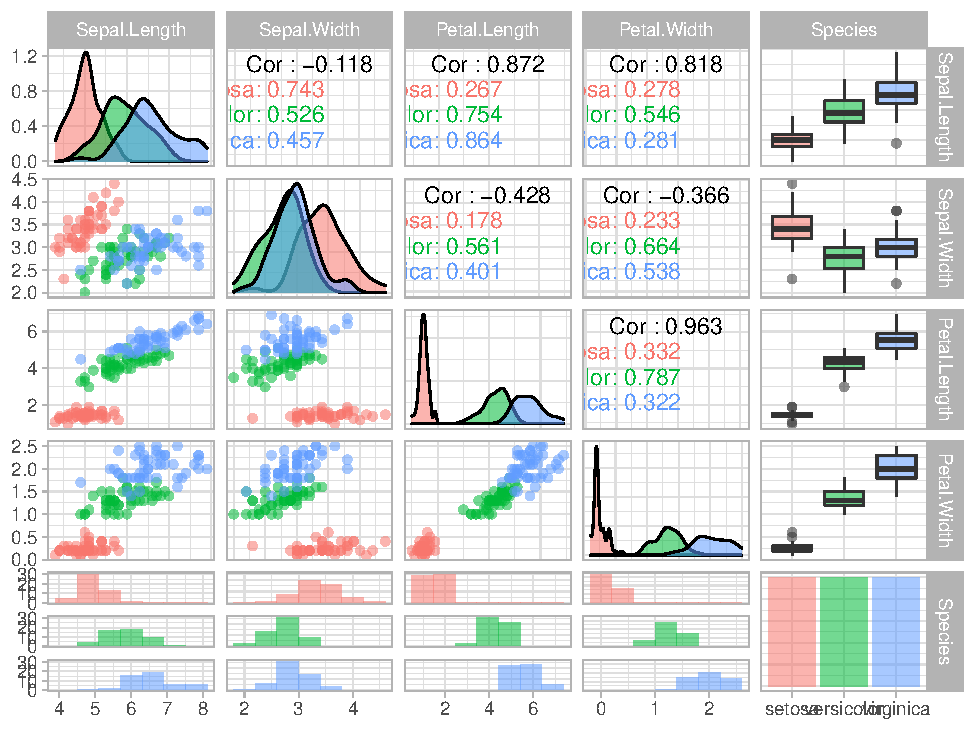
\includegraphics[width=1\linewidth]{_main_files/figure-latex/unnamed-chunk-2-1} \end{center}

De estos análisis observamos, por ejemplo, que 2 de las 4 variables---\emph{Petal.Width} y \emph{Petal.Length}---parecen separar bastante bien las 3 especies, y que la muestra está muy bien balanceada.

Antes de pasar a ajustar nuestro modelo, debemos \emph{preprocesar} la muestra. El algoritmo \emph{KNN} es muy sensible a la escala de los datos, por ejemplo, podría favorecer distancias entre elementos con valores más grandes. Una forma sencilla de \emph{estandarizar} o \emph{escalar} los datos es usando:

\begin{Shaded}
\begin{Highlighting}[]
\NormalTok{iris.scl <-}\StringTok{ }\KeywordTok{scale}\NormalTok{(iris[,}\DecValTok{1}\OperatorTok{:}\DecValTok{4}\NormalTok{])}
\end{Highlighting}
\end{Shaded}

Otro elemento importante es la validación del modelo que ajustemos: ¿cómo y con qué muestra medir la precisión? Por lo pronto, fijaremos aleatoriamente un 20\% de los datos para calcular la \emph{tasa de error}.

\begin{Shaded}
\begin{Highlighting}[]
\CommentTok{# set de índices para entrenar-validar (80% - 20%)}
\KeywordTok{set.seed}\NormalTok{(}\DecValTok{123}\NormalTok{)}
\NormalTok{train.ID <-}\StringTok{ }\KeywordTok{sample}\NormalTok{(}\DecValTok{1}\OperatorTok{:}\KeywordTok{nrow}\NormalTok{(iris), }\FloatTok{0.8} \OperatorTok{*}\StringTok{ }\KeywordTok{nrow}\NormalTok{(iris)) }

\CommentTok{# matriz de diseño para entrenar}
\NormalTok{X.train <-}\StringTok{ }\NormalTok{iris.scl[train.ID,}\DecValTok{1}\OperatorTok{:}\DecValTok{4}\NormalTok{]}
\CommentTok{# matriz de diseño para testear}
\NormalTok{X.test <-}\StringTok{ }\NormalTok{iris.scl[}\OperatorTok{-}\NormalTok{train.ID,}\DecValTok{1}\OperatorTok{:}\DecValTok{4}\NormalTok{]}
\CommentTok{# respuesta (categórica) entrenamiento}
\NormalTok{Y <-}\StringTok{ }\NormalTok{iris[train.ID,}\DecValTok{5}\NormalTok{]}
\CommentTok{# respuesta (categórica) test}
\NormalTok{Y.test <-}\StringTok{ }\NormalTok{iris[}\OperatorTok{-}\NormalTok{train.ID,}\DecValTok{5}\NormalTok{]}
\end{Highlighting}
\end{Shaded}

Usando la función \texttt{knn} podemos predecir las clases de los datos en \texttt{X.test}. Otro problema es cómo seleccionar la cantidad de vecinos \texttt{k} apropiada. Una \emph{regla de pulgar} (\emph{thumb rule}) es fijar \(k = \sqrt{n_{train}}\). Para analizar la precisión del modelo creamos la \emph{matriz de confusión} y calculamos la tasa de error correspondiente para el conjunto de datos test.

\begin{Shaded}
\begin{Highlighting}[]
\CommentTok{# KNN }
\NormalTok{pr <-}\StringTok{ }\KeywordTok{knn}\NormalTok{(X.train, X.test, }\DataTypeTok{cl=}\NormalTok{Y, }\DataTypeTok{k =} \KeywordTok{round}\NormalTok{(}\KeywordTok{sqrt}\NormalTok{(}\KeywordTok{nrow}\NormalTok{(X.train))))}

\CommentTok{# matriz de confusión}
\NormalTok{tab <-}\StringTok{ }\KeywordTok{table}\NormalTok{(pr,Y.test)}
\end{Highlighting}
\end{Shaded}

\begin{table}

\caption{\label{tab:confIris-tab}Matriz de Confusión - KNN Iris}
\centering
\begin{tabular}[t]{lrrr}
\toprule
  & setosa & versicolor & virginica\\
\midrule
setosa & 10 & 0 & 0\\
versicolor & 0 & 14 & 0\\
virginica & 0 & 1 & 5\\
\bottomrule
\end{tabular}
\end{table}

\begin{Shaded}
\begin{Highlighting}[]
\CommentTok{# tasa de error test}
\NormalTok{test.error <-}\StringTok{ }\KeywordTok{sum}\NormalTok{(pr }\OperatorTok{!=}\StringTok{ }\NormalTok{Y.test)}\OperatorTok{/}\KeywordTok{sum}\NormalTok{(tab)}
\NormalTok{test.error}
\end{Highlighting}
\end{Shaded}

\begin{verbatim}
## [1] 0.03333333
\end{verbatim}

La tasa de error test es bastante baja, además indica que se clasifican bien el \(\approx 97\%\) de las observaciones. Veamos ahora qué pasa al variar el número de vecinos \texttt{K}.

\begin{Shaded}
\begin{Highlighting}[]
\NormalTok{test.error <-}\StringTok{ }\KeywordTok{data.frame}\NormalTok{()}
\ControlFlowTok{for}\NormalTok{ (K }\ControlFlowTok{in} \KeywordTok{seq}\NormalTok{(}\DecValTok{1}\NormalTok{, }\DecValTok{120}\NormalTok{, }\DataTypeTok{by =} \DecValTok{5}\NormalTok{)) \{}
  \CommentTok{# KNN}
\NormalTok{  pr <-}\StringTok{ }\KeywordTok{knn}\NormalTok{(X.train,X.test,}\DataTypeTok{cl=}\NormalTok{Y,}\DataTypeTok{k=}\NormalTok{K)}
  \CommentTok{# matriz de confusion}
\NormalTok{  tab <-}\StringTok{ }\KeywordTok{table}\NormalTok{(pr,Y.test)}
  \CommentTok{# tasa de error test}
\NormalTok{  test.error <-}\StringTok{ }\KeywordTok{rbind}\NormalTok{(test.error, }
                        \KeywordTok{data.frame}\NormalTok{(}\DataTypeTok{Tasa.Error =} \KeywordTok{sum}\NormalTok{(pr }\OperatorTok{!=}\StringTok{ }\NormalTok{Y.test)}\OperatorTok{/}\KeywordTok{sum}\NormalTok{(tab), K))}
\NormalTok{\}}

\KeywordTok{ggplot}\NormalTok{(test.error, }\KeywordTok{aes}\NormalTok{(}\DataTypeTok{x =}\NormalTok{ K, }\DataTypeTok{y =}\NormalTok{ Tasa.Error)) }\OperatorTok{+}\StringTok{ }
\StringTok{  }\KeywordTok{geom_point}\NormalTok{() }\OperatorTok{+}\StringTok{ }
\StringTok{  }\KeywordTok{geom_line}\NormalTok{() }\OperatorTok{+}\StringTok{ }
\StringTok{  }\KeywordTok{ylab}\NormalTok{(}\StringTok{"Tasa de Error (test)"}\NormalTok{) }\OperatorTok{+}\StringTok{  }\KeywordTok{xlab}\NormalTok{(}\StringTok{"K: número de vecinos"}\NormalTok{) }\OperatorTok{+}\StringTok{ }
\StringTok{  }\KeywordTok{theme_light}\NormalTok{()}
\end{Highlighting}
\end{Shaded}

\begin{center}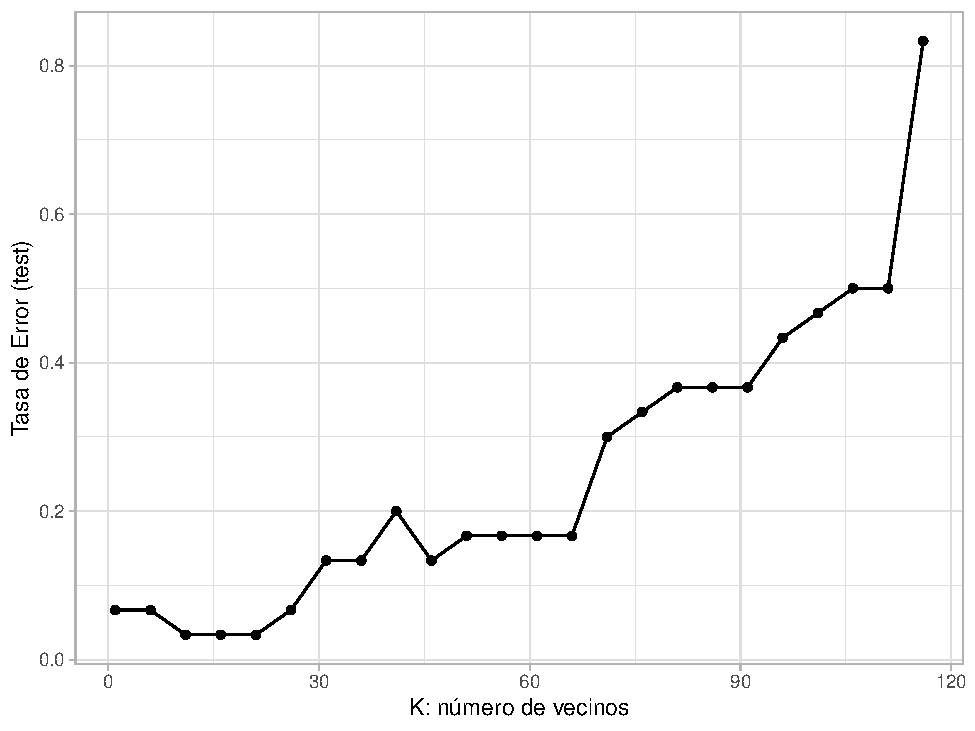
\includegraphics[width=0.8\linewidth]{_main_files/figure-latex/unnamed-chunk-7-1} \end{center}

Se representa la tasa de error al aumentar el número de vecinos. Los \emph{saltos} de la curva son resultado del pequeño tamaño de la muestra test. Como cualquier otro modelo de machine learning, el interés está en seleccionar el nivel de flexibilidad (número de vecinos) que mejore la clasificación\ldots{} inténtalo!

\hypertarget{el-paquete-caret}{%
\section{\texorpdfstring{El paquete \texttt{caret}}{El paquete caret}}\label{el-paquete-caret}}

El paquete \texttt{caret} (\emph{\textbf{C}lassification \textbf{A}nd \textbf{RE}gression \textbf{T}raining}) es uno de los más populares para entrenar modelos de \emph{machine learning}. Contiene una interface uniforme para la mayoría de los algoritmos que se tratan en este curso y, en particular, los 3 que veremos en estas sesiones. Las ventajas del paquete son que permite hacer:

\begin{itemize}
\tightlist
\item
  partición de los datos
\item
  pre-procesado de los datos
\item
  selección de variables
\item
  ajuste del modelo usando remuestreo
\item
  estimación de la importancia/relevancia de las variables
\end{itemize}

Más información disponible en \href{http://topepo.github.io/caret/index.html}{topepo.github.io/caret}.

\hypertarget{visualizaciuxf3n}{%
\subsection{Visualización}\label{visualizaciuxf3n}}

Seguiremos con los datos \texttt{iris}. El paso inicial: análisis descriptivo y visualización de los datos podríamos obviarlo\ldots{} pero a modo didáctico reproducimos el mismo análisis, esta vez usando la función \texttt{featurePlot} de \texttt{caret}.

\begin{Shaded}
\begin{Highlighting}[]
\KeywordTok{library}\NormalTok{(caret)}
\KeywordTok{str}\NormalTok{(iris)}
\end{Highlighting}
\end{Shaded}

\begin{verbatim}
## 'data.frame':    150 obs. of  5 variables:
##  $ Sepal.Length: num  5.1 4.9 4.7 4.6 5 5.4 4.6 5 4.4 4.9 ...
##  $ Sepal.Width : num  3.5 3 3.2 3.1 3.6 3.9 3.4 3.4 2.9 3.1 ...
##  $ Petal.Length: num  1.4 1.4 1.3 1.5 1.4 1.7 1.4 1.5 1.4 1.5 ...
##  $ Petal.Width : num  0.2 0.2 0.2 0.2 0.2 0.4 0.3 0.2 0.2 0.1 ...
##  $ Species     : Factor w/ 3 levels "setosa","versicolor",..: 1 1 1 1 1 1 1 1 1 1 ...
\end{verbatim}

Diagramas de dispersión:

\begin{Shaded}
\begin{Highlighting}[]
\KeywordTok{featurePlot}\NormalTok{(}\DataTypeTok{x =}\NormalTok{ iris[, }\DecValTok{1}\OperatorTok{:}\DecValTok{4}\NormalTok{], }
            \DataTypeTok{y =}\NormalTok{ iris}\OperatorTok{$}\NormalTok{Species, }
            \DataTypeTok{plot =} \StringTok{"pairs"}\NormalTok{,}
            \CommentTok{## Add a key at the top}
            \DataTypeTok{auto.key =} \KeywordTok{list}\NormalTok{(}\DataTypeTok{columns =} \DecValTok{3}\NormalTok{))}
\end{Highlighting}
\end{Shaded}

\begin{center}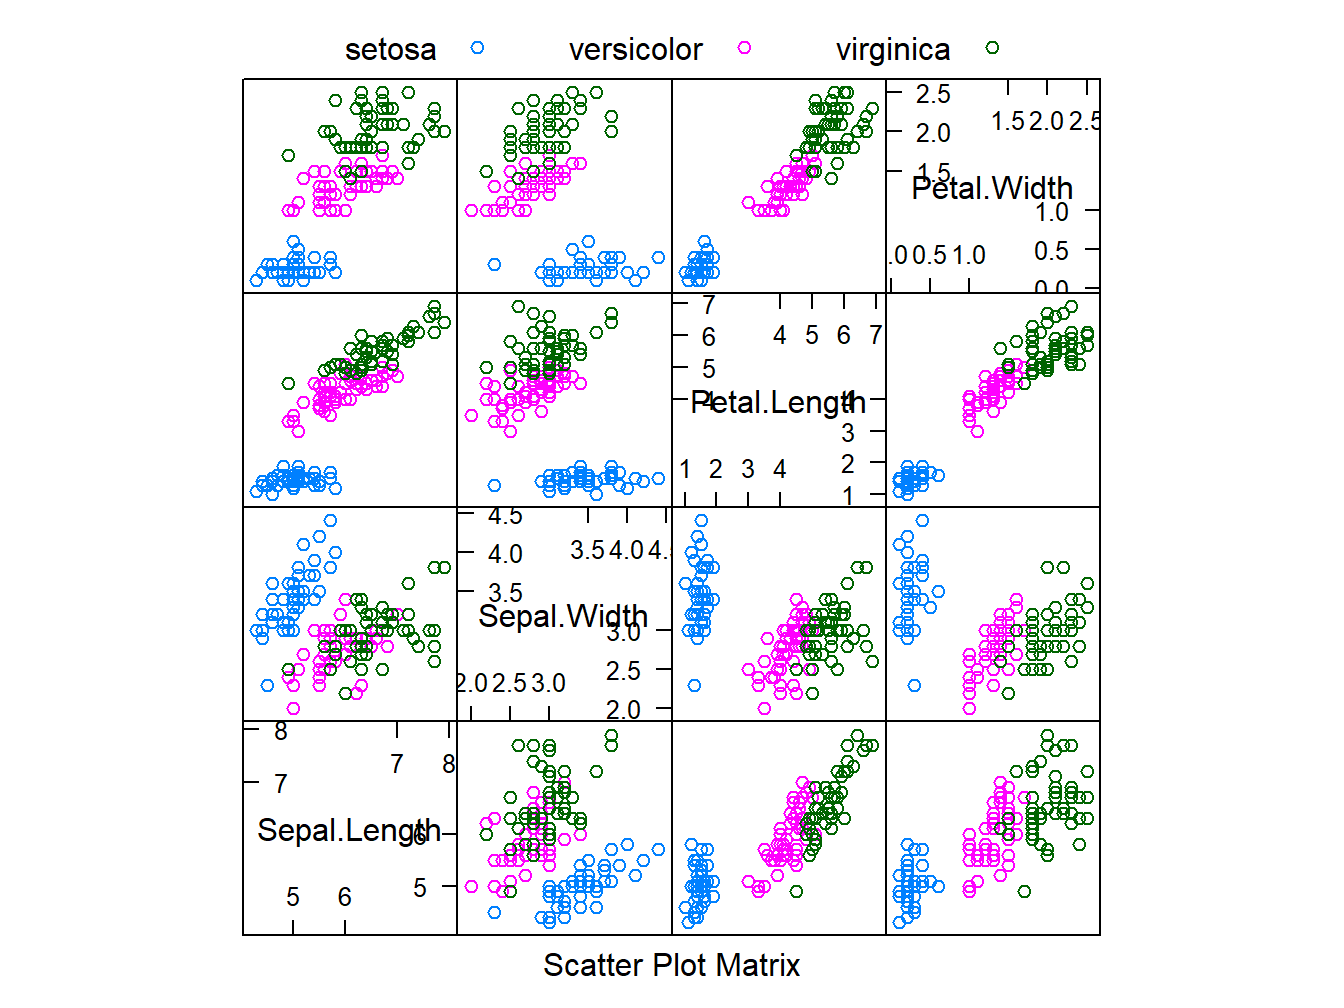
\includegraphics[width=0.8\linewidth]{_main_files/figure-latex/unnamed-chunk-9-1} \end{center}

Densidades estimadas:

\begin{Shaded}
\begin{Highlighting}[]
\KeywordTok{featurePlot}\NormalTok{(}\DataTypeTok{x =}\NormalTok{ iris[, }\DecValTok{1}\OperatorTok{:}\DecValTok{4}\NormalTok{], }
            \DataTypeTok{y =}\NormalTok{ iris}\OperatorTok{$}\NormalTok{Species,}
            \DataTypeTok{plot =} \StringTok{"density"}\NormalTok{, }
            \CommentTok{## Pass in options to xyplot() to }
            \CommentTok{## make it prettier}
            \DataTypeTok{scales =} \KeywordTok{list}\NormalTok{(}\DataTypeTok{x =} \KeywordTok{list}\NormalTok{(}\DataTypeTok{relation=}\StringTok{"free"}\NormalTok{), }
                          \DataTypeTok{y =} \KeywordTok{list}\NormalTok{(}\DataTypeTok{relation=}\StringTok{"free"}\NormalTok{)), }
            \DataTypeTok{adjust =} \FloatTok{1.5}\NormalTok{, }
            \DataTypeTok{pch =} \StringTok{"|"}\NormalTok{, }
            \DataTypeTok{layout =} \KeywordTok{c}\NormalTok{(}\DecValTok{4}\NormalTok{, }\DecValTok{1}\NormalTok{), }
            \DataTypeTok{auto.key =} \KeywordTok{list}\NormalTok{(}\DataTypeTok{columns =} \DecValTok{3}\NormalTok{))}
\end{Highlighting}
\end{Shaded}

\begin{center}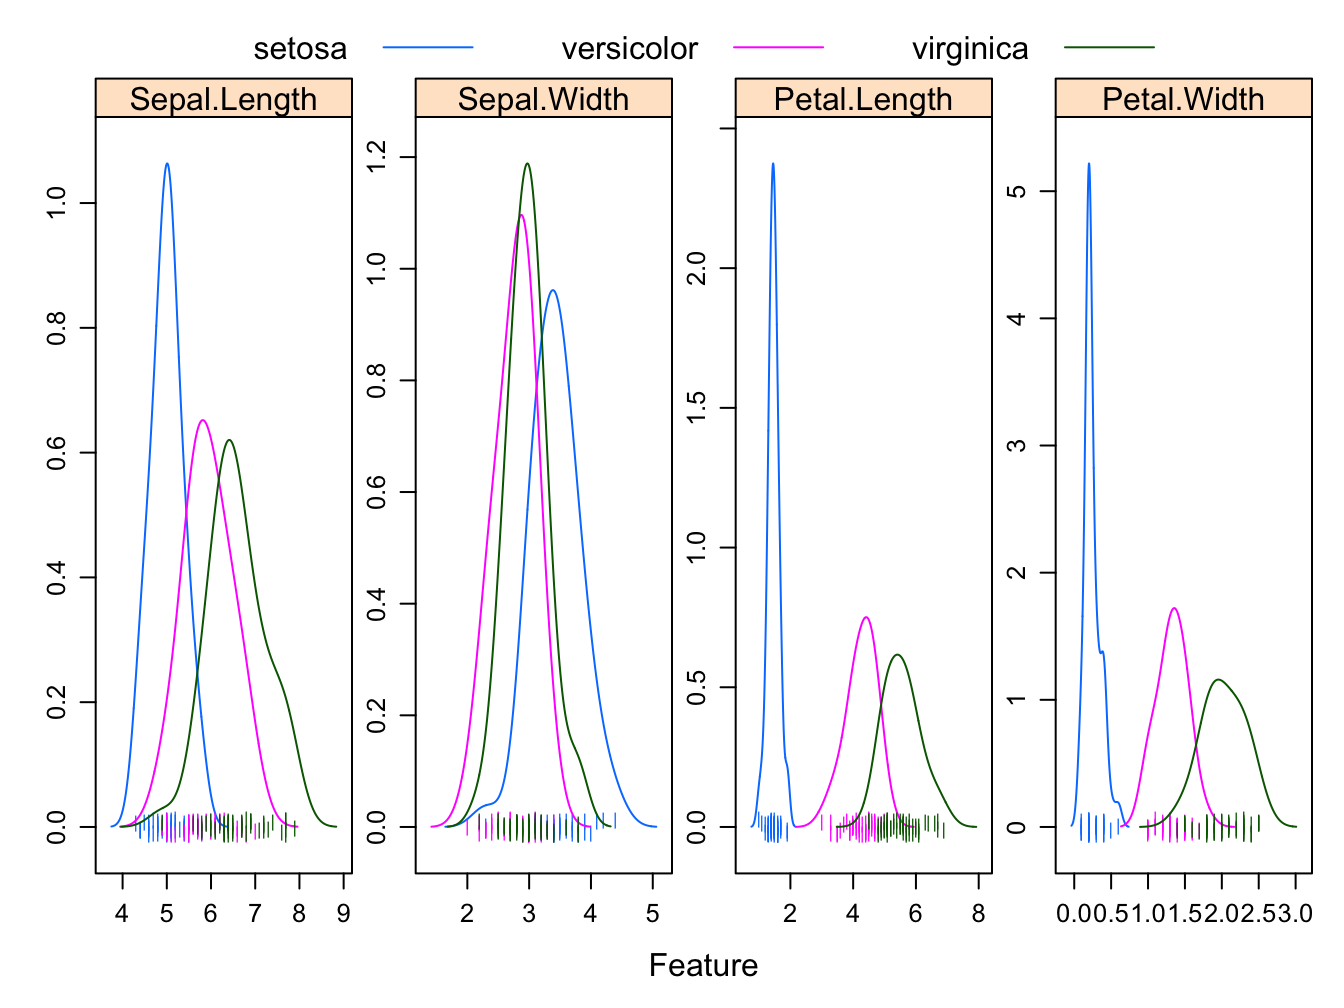
\includegraphics[width=0.8\linewidth]{_main_files/figure-latex/unnamed-chunk-10-1} \end{center}

Diagramas de cajas:

\begin{Shaded}
\begin{Highlighting}[]
\KeywordTok{featurePlot}\NormalTok{(}\DataTypeTok{x =}\NormalTok{ iris[, }\DecValTok{1}\OperatorTok{:}\DecValTok{4}\NormalTok{], }
            \DataTypeTok{y =}\NormalTok{ iris}\OperatorTok{$}\NormalTok{Species, }
            \DataTypeTok{plot =} \StringTok{"box"}\NormalTok{, }
            \CommentTok{## Pass in options to bwplot() }
            \DataTypeTok{scales =} \KeywordTok{list}\NormalTok{(}\DataTypeTok{y =} \KeywordTok{list}\NormalTok{(}\DataTypeTok{relation=}\StringTok{"free"}\NormalTok{),}
                          \DataTypeTok{x =} \KeywordTok{list}\NormalTok{(}\DataTypeTok{rot =} \DecValTok{90}\NormalTok{)),  }
            \DataTypeTok{layout =} \KeywordTok{c}\NormalTok{(}\DecValTok{4}\NormalTok{,}\DecValTok{1}\NormalTok{ ), }
            \DataTypeTok{auto.key =} \KeywordTok{list}\NormalTok{(}\DataTypeTok{columns =} \DecValTok{2}\NormalTok{))}
\end{Highlighting}
\end{Shaded}

\begin{center}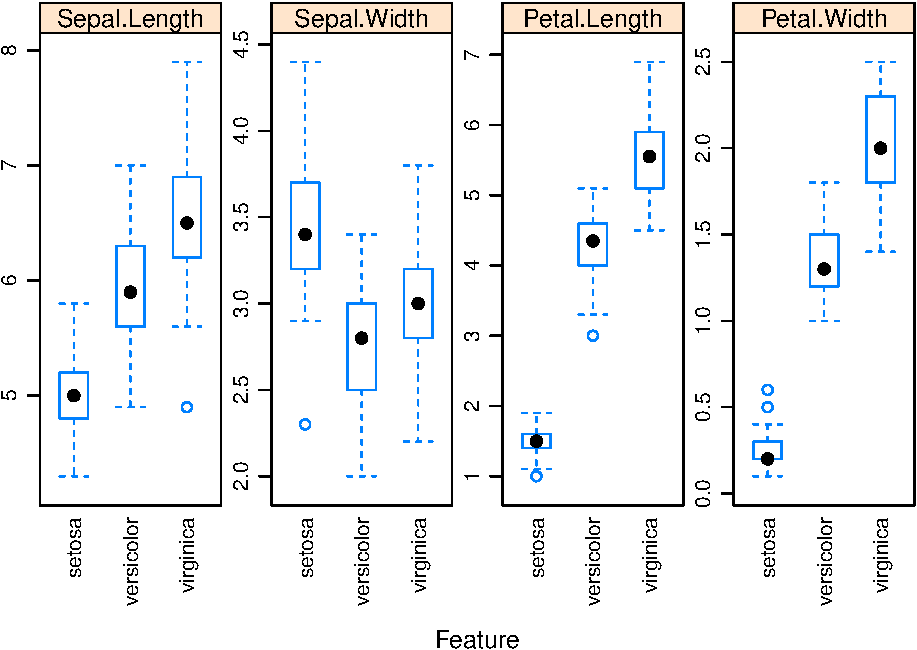
\includegraphics[width=0.8\linewidth]{_main_files/figure-latex/unnamed-chunk-11-1} \end{center}

\hypertarget{clasificaciuxf3n-con-knn}{%
\subsection{Clasificación con KNN}\label{clasificaciuxf3n-con-knn}}

Necesitamos extraer una muestra independiente (\emph{test}) para probar el modelo, una vez ajustado. Ahora usaremos la función \texttt{createDataPartition}, que permite hacer la partición teniendo en cuenta la variable respuesta. Esto es esencial para mantener el balance de la muestra.

\begin{Shaded}
\begin{Highlighting}[]
\CommentTok{# creamos una partición test}
\NormalTok{df <-}\StringTok{ }\NormalTok{iris}
\KeywordTok{set.seed}\NormalTok{(}\DecValTok{123}\NormalTok{)}
\NormalTok{train.ID <-}\StringTok{ }\KeywordTok{createDataPartition}\NormalTok{(df}\OperatorTok{$}\NormalTok{Species, }\DataTypeTok{p =} \FloatTok{0.8}\NormalTok{, }\DataTypeTok{list =} \OtherTok{FALSE}\NormalTok{)}

\NormalTok{train_df <-}\StringTok{ }\NormalTok{df[train.ID, ]}
\NormalTok{test_df <-}\StringTok{ }\NormalTok{df[}\OperatorTok{-}\NormalTok{train.ID, ]}
\end{Highlighting}
\end{Shaded}

Para ajustar el modelo usaremos la función \texttt{train}, que permite:
* evaluar, usando remuestreo, el efecto de distintos parámetros en la precisión del modelo
* escoger el modelo óptimo, de acuerdo a los parámetros probados
* estimar la precisión del modelo, de acuerdo a diferentes medidas

Actualmente hay uno \(\approx 238\) modelos disponibles. Nosotros empezaremos probando el \texttt{knn}, pero antes tenemos que especificar el método de remuestreo, usando la función \texttt{trainControl}. Con esta función, podemos fijar una validación cruzada \emph{k-Fold} o \emph{leave-one-out (LOOCV)}. También están disponibles las opciones \emph{bootstrap} y \emph{k-Fold repetitivo}.

En este ejemplo, hemos fijado un \emph{k-Fold} con 10 hojas. Además, hacemos el escalado de las variables dentro del propio algoritmo, usando la opción \texttt{preProcess}. Finalmente, le decimos al algoritmo que intente 10 valores diferentes para escoger el número de vecinos óptimo, usando la opción \texttt{tuneLength}

\begin{Shaded}
\begin{Highlighting}[]
\CommentTok{# primeros pasos con la validación cruzada...}
\NormalTok{fit_control <-}\StringTok{ }\KeywordTok{trainControl}\NormalTok{(}\DataTypeTok{method=}\StringTok{'cv'}\NormalTok{, }\DataTypeTok{number =} \DecValTok{10}\NormalTok{)  }

\NormalTok{model_knn_iris <-}\StringTok{ }\KeywordTok{train}\NormalTok{(Species }\OperatorTok{~}\NormalTok{., }
                       \DataTypeTok{data =}\NormalTok{ train_df, }
                       \DataTypeTok{method =} \StringTok{"knn"}\NormalTok{, }
                       \DataTypeTok{trControl =}\NormalTok{ fit_control, }
                       \DataTypeTok{preProcess =} \KeywordTok{c}\NormalTok{(}\StringTok{"center"}\NormalTok{, }\StringTok{"scale"}\NormalTok{),  }
                       \DataTypeTok{tuneLength =} \DecValTok{10}\NormalTok{)}
\NormalTok{model_knn_iris}
\end{Highlighting}
\end{Shaded}

\begin{verbatim}
## k-Nearest Neighbors 
## 
## 120 samples
##   4 predictor
##   3 classes: 'setosa', 'versicolor', 'virginica' 
## 
## Pre-processing: centered (4), scaled (4) 
## Resampling: Cross-Validated (10 fold) 
## Summary of sample sizes: 108, 108, 108, 108, 108, 108, ... 
## Resampling results across tuning parameters:
## 
##   k   Accuracy   Kappa 
##    5  0.9666667  0.9500
##    7  0.9583333  0.9375
##    9  0.9750000  0.9625
##   11  0.9583333  0.9375
##   13  0.9583333  0.9375
##   15  0.9583333  0.9375
##   17  0.9583333  0.9375
##   19  0.9416667  0.9125
##   21  0.9500000  0.9250
##   23  0.9333333  0.9000
## 
## Accuracy was used to select the optimal model using the largest value.
## The final value used for the model was k = 9.
\end{verbatim}

\begin{Shaded}
\begin{Highlighting}[]
\KeywordTok{plot}\NormalTok{(model_knn_iris)}
\end{Highlighting}
\end{Shaded}

\begin{center}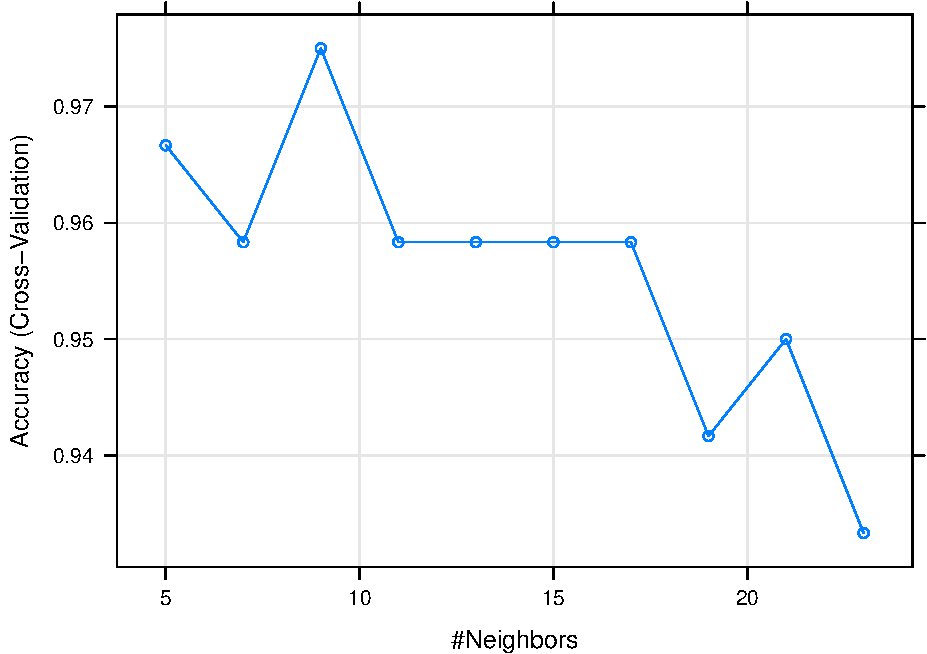
\includegraphics[width=0.8\linewidth]{_main_files/figure-latex/unnamed-chunk-13-1} \end{center}

Podemos ver en el resumen el número óptimo de vecinos (entre los valores probados) del modelo final. En el gráfico, vemos cómo varía el \emph{accuracy} en función del número de vecinos. La tabla de confusión y medidas de precisión para los datos test:

\begin{Shaded}
\begin{Highlighting}[]
\CommentTok{# hagamos las predicciones del conjunto de prueba}
\NormalTok{prediction_knn_iris <-}\StringTok{ }\KeywordTok{predict}\NormalTok{(model_knn_iris, }\DataTypeTok{newdata =}\NormalTok{ test_df)}
\KeywordTok{confusionMatrix}\NormalTok{(prediction_knn_iris, }\DataTypeTok{reference =}\NormalTok{ test_df}\OperatorTok{$}\NormalTok{Species)}
\end{Highlighting}
\end{Shaded}

\begin{verbatim}
## Confusion Matrix and Statistics
## 
##             Reference
## Prediction   setosa versicolor virginica
##   setosa         10          0         0
##   versicolor      0         10         2
##   virginica       0          0         8
## 
## Overall Statistics
##                                           
##                Accuracy : 0.9333          
##                  95% CI : (0.7793, 0.9918)
##     No Information Rate : 0.3333          
##     P-Value [Acc > NIR] : 8.747e-12       
##                                           
##                   Kappa : 0.9             
##                                           
##  Mcnemar's Test P-Value : NA              
## 
## Statistics by Class:
## 
##                      Class: setosa Class: versicolor Class: virginica
## Sensitivity                 1.0000            1.0000           0.8000
## Specificity                 1.0000            0.9000           1.0000
## Pos Pred Value              1.0000            0.8333           1.0000
## Neg Pred Value              1.0000            1.0000           0.9091
## Prevalence                  0.3333            0.3333           0.3333
## Detection Rate              0.3333            0.3333           0.2667
## Detection Prevalence        0.3333            0.4000           0.2667
## Balanced Accuracy           1.0000            0.9500           0.9000
\end{verbatim}

Intentemos ahora fijar las cantidades de vecinos a probar. También cambiamos el método de remuestreo\ldots{}

\begin{Shaded}
\begin{Highlighting}[]
\CommentTok{# definimos el grid:}
\NormalTok{some_k <-}\StringTok{ }\KeywordTok{expand.grid}\NormalTok{(}\DataTypeTok{k =} \DecValTok{1}\OperatorTok{:}\DecValTok{15}\NormalTok{) }

\CommentTok{# k-fold CV pero con repeticiones}
\NormalTok{fit_control1 <-}\StringTok{ }\KeywordTok{trainControl}\NormalTok{(}
  \DataTypeTok{method =} \StringTok{"repeatedcv"}\NormalTok{, }
  \DataTypeTok{number =} \DecValTok{10}\NormalTok{, }\CommentTok{# número de folds}
  \DataTypeTok{repeats =} \DecValTok{5}\NormalTok{ ) }\CommentTok{# repeticiones}

\CommentTok{# bootstrap}
\NormalTok{fit_control2 <-}\StringTok{ }\KeywordTok{trainControl}\NormalTok{(}
  \DataTypeTok{method =} \StringTok{"boot"}\NormalTok{,  }
  \DataTypeTok{number =} \DecValTok{10}\NormalTok{) }\CommentTok{# número de muestras bootstrap}

\CommentTok{# LOOCV}
\NormalTok{fit_control3 <-}\StringTok{ }\KeywordTok{trainControl}\NormalTok{(}
  \DataTypeTok{method =} \StringTok{"LOOCV"}\NormalTok{) }

\NormalTok{model2_knn_iris <-}\StringTok{ }\KeywordTok{train}\NormalTok{(Species }\OperatorTok{~}\NormalTok{., }
                        \DataTypeTok{data =}\NormalTok{ train_df, }
                        \DataTypeTok{method =} \StringTok{"knn"}\NormalTok{, }
                        \DataTypeTok{trControl =}\NormalTok{ fit_control2, }
                        \DataTypeTok{preProcess =} \KeywordTok{c}\NormalTok{(}\StringTok{"center"}\NormalTok{, }\StringTok{"scale"}\NormalTok{),  }
                        \DataTypeTok{tuneGrid =}\NormalTok{ some_k)}
\NormalTok{model2_knn_iris}
\end{Highlighting}
\end{Shaded}

\begin{verbatim}
## k-Nearest Neighbors 
## 
## 120 samples
##   4 predictor
##   3 classes: 'setosa', 'versicolor', 'virginica' 
## 
## Pre-processing: centered (4), scaled (4) 
## Resampling: Bootstrapped (10 reps) 
## Summary of sample sizes: 120, 120, 120, 120, 120, 120, ... 
## Resampling results across tuning parameters:
## 
##   k   Accuracy   Kappa    
##    1  0.9481717  0.9211545
##    2  0.9475159  0.9196833
##    3  0.9453882  0.9165257
##    4  0.9599231  0.9393154
##    5  0.9665503  0.9492382
##    6  0.9686637  0.9524826
##    7  0.9688968  0.9528083
##    8  0.9596084  0.9388259
##    9  0.9647549  0.9465745
##   10  0.9600366  0.9392605
##   11  0.9624756  0.9431153
##   12  0.9555270  0.9326274
##   13  0.9623479  0.9429620
##   14  0.9439143  0.9151811
##   15  0.9438559  0.9150458
## 
## Accuracy was used to select the optimal model using the largest value.
## The final value used for the model was k = 7.
\end{verbatim}

\begin{Shaded}
\begin{Highlighting}[]
\KeywordTok{plot}\NormalTok{(model2_knn_iris)}
\end{Highlighting}
\end{Shaded}

\begin{center}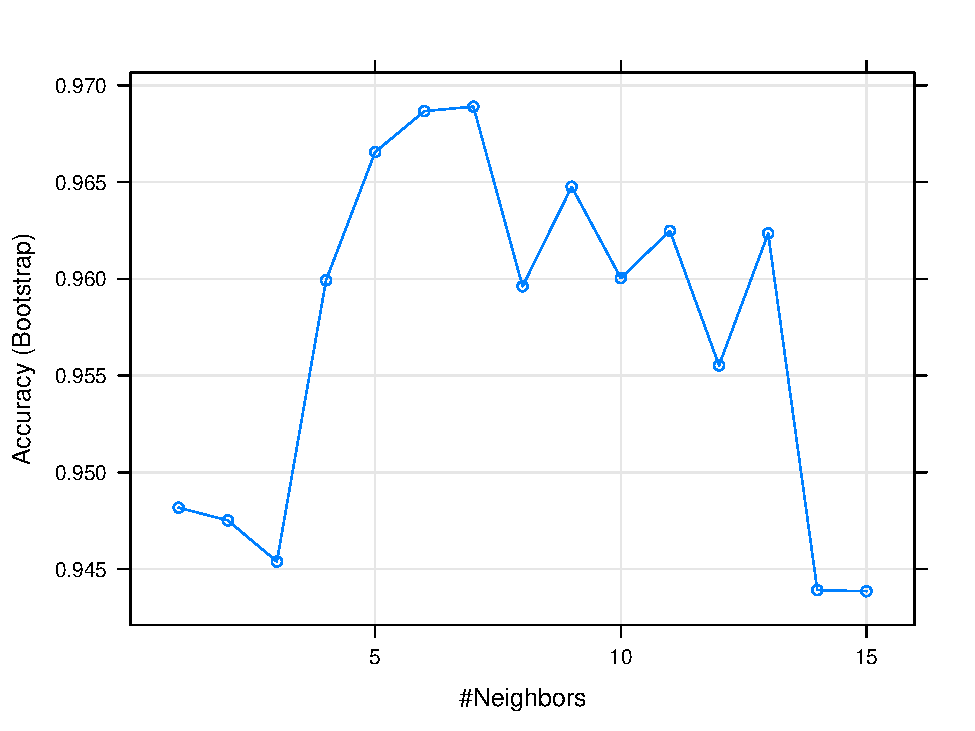
\includegraphics[width=0.8\linewidth]{_main_files/figure-latex/unnamed-chunk-15-1} \end{center}

\begin{Shaded}
\begin{Highlighting}[]
\CommentTok{# hagamos las predicciones del conjunto de prueba}
\NormalTok{prediction_knn_iris2 <-}\StringTok{ }\KeywordTok{predict}\NormalTok{(model2_knn_iris, }\DataTypeTok{newdata =}\NormalTok{ test_df)}
\KeywordTok{confusionMatrix}\NormalTok{(prediction_knn_iris2, }\DataTypeTok{reference =}\NormalTok{ test_df}\OperatorTok{$}\NormalTok{Species)}
\end{Highlighting}
\end{Shaded}

\begin{verbatim}
## Confusion Matrix and Statistics
## 
##             Reference
## Prediction   setosa versicolor virginica
##   setosa         10          0         0
##   versicolor      0         10         2
##   virginica       0          0         8
## 
## Overall Statistics
##                                           
##                Accuracy : 0.9333          
##                  95% CI : (0.7793, 0.9918)
##     No Information Rate : 0.3333          
##     P-Value [Acc > NIR] : 8.747e-12       
##                                           
##                   Kappa : 0.9             
##                                           
##  Mcnemar's Test P-Value : NA              
## 
## Statistics by Class:
## 
##                      Class: setosa Class: versicolor Class: virginica
## Sensitivity                 1.0000            1.0000           0.8000
## Specificity                 1.0000            0.9000           1.0000
## Pos Pred Value              1.0000            0.8333           1.0000
## Neg Pred Value              1.0000            1.0000           0.9091
## Prevalence                  0.3333            0.3333           0.3333
## Detection Rate              0.3333            0.3333           0.2667
## Detection Prevalence        0.3333            0.4000           0.2667
## Balanced Accuracy           1.0000            0.9500           0.9000
\end{verbatim}

\hypertarget{importancia-de-las-variables}{%
\subsection{Importancia de las variables}\label{importancia-de-las-variables}}

Para KNN no tenemos un método que permita determinar la relevancia de cada predictor. Por ejemplo, en mínimos cuadrados, sí se puede conducir un test para determinar si cada coeficiente \(\beta_i\) del modelo es significativamente distinto de cero. Aún así, \texttt{caret} incorpora la función \texttt{varImp} que da una medida de \emph{importancia} de cada predictor del problema de clasificación o regresión.

\begin{Shaded}
\begin{Highlighting}[]
\KeywordTok{varImp}\NormalTok{(model_knn_iris)}
\end{Highlighting}
\end{Shaded}

\begin{verbatim}
## ROC curve variable importance
## 
##   variables are sorted by maximum importance across the classes
##              setosa versicolor virginica
## Petal.Width  100.00     100.00     100.0
## Petal.Length 100.00     100.00     100.0
## Sepal.Length  90.80      72.07      90.8
## Sepal.Width   56.32      56.32       0.0
\end{verbatim}

Aunque esto no debe usarse como método de selección de variables, sí motiva el estudio del problema al disminuir la dimensión \(p = 4\). Por ejemplo, veamos la precisión del modelo al dejar solo \texttt{Petal.Length} y \texttt{Petal.Width}.

\begin{Shaded}
\begin{Highlighting}[]
\CommentTok{# seleccionamos los predictores que queremos y la respuesta}
\NormalTok{df_petal <-}\StringTok{ }\NormalTok{iris[,}\KeywordTok{c}\NormalTok{(}\StringTok{"Petal.Length"}\NormalTok{, }\StringTok{"Petal.Width"}\NormalTok{, }\StringTok{"Species"}\NormalTok{)]}
\NormalTok{train_df_petal <-}\StringTok{ }\NormalTok{df_petal[train.ID, ]}
\NormalTok{test_df_petal <-}\StringTok{ }\NormalTok{df_petal[}\OperatorTok{-}\NormalTok{train.ID, ]}

\CommentTok{# el modelo...}
\NormalTok{fit_control <-}\StringTok{ }\KeywordTok{trainControl}\NormalTok{(}\DataTypeTok{method=}\StringTok{'cv'}\NormalTok{, }\DataTypeTok{number =} \DecValTok{10}\NormalTok{)  }

\NormalTok{model_knn_petal <-}\StringTok{ }\KeywordTok{train}\NormalTok{(Species }\OperatorTok{~}\NormalTok{., }
                        \DataTypeTok{data =}\NormalTok{ train_df_petal, }
                        \DataTypeTok{method =} \StringTok{"knn"}\NormalTok{, }
                        \DataTypeTok{trControl =}\NormalTok{ fit_control, }
                        \DataTypeTok{preProcess =} \KeywordTok{c}\NormalTok{(}\StringTok{"center"}\NormalTok{, }\StringTok{"scale"}\NormalTok{),  }
                        \DataTypeTok{tuneLength =} \DecValTok{20}\NormalTok{)}
\NormalTok{model_knn_petal}
\end{Highlighting}
\end{Shaded}

\begin{verbatim}
## k-Nearest Neighbors 
## 
## 120 samples
##   2 predictor
##   3 classes: 'setosa', 'versicolor', 'virginica' 
## 
## Pre-processing: centered (2), scaled (2) 
## Resampling: Cross-Validated (10 fold) 
## Summary of sample sizes: 108, 108, 108, 108, 108, 108, ... 
## Resampling results across tuning parameters:
## 
##   k   Accuracy   Kappa 
##    5  0.9666667  0.9500
##    7  0.9666667  0.9500
##    9  0.9666667  0.9500
##   11  0.9666667  0.9500
##   13  0.9666667  0.9500
##   15  0.9666667  0.9500
##   17  0.9583333  0.9375
##   19  0.9666667  0.9500
##   21  0.9583333  0.9375
##   23  0.9666667  0.9500
##   25  0.9666667  0.9500
##   27  0.9666667  0.9500
##   29  0.9666667  0.9500
##   31  0.9666667  0.9500
##   33  0.9750000  0.9625
##   35  0.9833333  0.9750
##   37  0.9750000  0.9625
##   39  0.9833333  0.9750
##   41  0.9750000  0.9625
##   43  0.9666667  0.9500
## 
## Accuracy was used to select the optimal model using the largest value.
## The final value used for the model was k = 39.
\end{verbatim}

\begin{Shaded}
\begin{Highlighting}[]
\KeywordTok{plot}\NormalTok{(model_knn_petal)}
\end{Highlighting}
\end{Shaded}

\begin{center}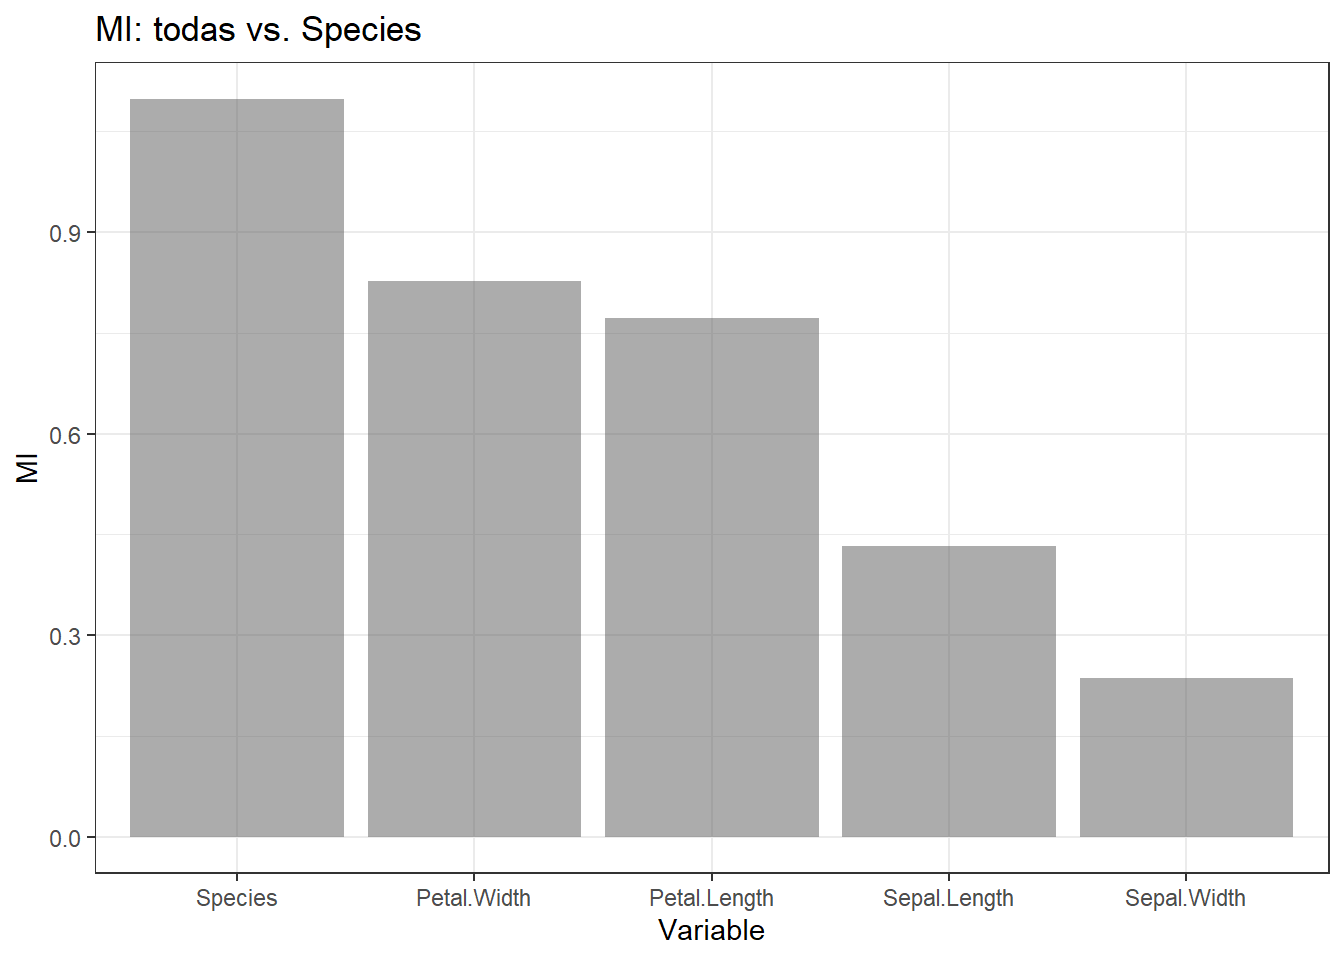
\includegraphics[width=0.8\linewidth]{_main_files/figure-latex/unnamed-chunk-18-1} \end{center}

\begin{Shaded}
\begin{Highlighting}[]
\CommentTok{# hagamos las predicciones del conjunto de prueba}
\NormalTok{prediction_knn_petal <-}\StringTok{ }\KeywordTok{predict}\NormalTok{(model_knn_petal, }\DataTypeTok{newdata =}\NormalTok{ test_df_petal)}
\KeywordTok{confusionMatrix}\NormalTok{(prediction_knn_petal, }\DataTypeTok{reference =}\NormalTok{ test_df_petal}\OperatorTok{$}\NormalTok{Species)}
\end{Highlighting}
\end{Shaded}

\begin{verbatim}
## Confusion Matrix and Statistics
## 
##             Reference
## Prediction   setosa versicolor virginica
##   setosa         10          0         0
##   versicolor      0         10         3
##   virginica       0          0         7
## 
## Overall Statistics
##                                           
##                Accuracy : 0.9             
##                  95% CI : (0.7347, 0.9789)
##     No Information Rate : 0.3333          
##     P-Value [Acc > NIR] : 1.665e-10       
##                                           
##                   Kappa : 0.85            
##                                           
##  Mcnemar's Test P-Value : NA              
## 
## Statistics by Class:
## 
##                      Class: setosa Class: versicolor Class: virginica
## Sensitivity                 1.0000            1.0000           0.7000
## Specificity                 1.0000            0.8500           1.0000
## Pos Pred Value              1.0000            0.7692           1.0000
## Neg Pred Value              1.0000            1.0000           0.8696
## Prevalence                  0.3333            0.3333           0.3333
## Detection Rate              0.3333            0.3333           0.2333
## Detection Prevalence        0.3333            0.4333           0.2333
## Balanced Accuracy           1.0000            0.9250           0.8500
\end{verbatim}

Pero, ¿cómo visualizar las fronteras de decisión del método? Ahora que \(p = 2\), podemos representar esto en el plano usando la siguiente función:

\begin{Shaded}
\begin{Highlighting}[]
\NormalTok{decision_bound =}\StringTok{ }\ControlFlowTok{function}\NormalTok{(train_df_in, test_df_in, model_in)\{}
  \CommentTok{# plot decision boundary  for iris[,c("Petal.Length", "Petal.Width", "Species")]}

  \KeywordTok{require}\NormalTok{(MASS)}
  \KeywordTok{require}\NormalTok{(caret)}
  \KeywordTok{require}\NormalTok{(ggplot2)}
  \KeywordTok{require}\NormalTok{(gridExtra)}

  \CommentTok{# Paso 1: crear un grid de valores desde min a max de ambos predictores}
\NormalTok{  pl =}\StringTok{ }\KeywordTok{seq}\NormalTok{(}\KeywordTok{min}\NormalTok{(train_df_in}\OperatorTok{$}\NormalTok{Petal.Length), }\KeywordTok{max}\NormalTok{(train_df_in}\OperatorTok{$}\NormalTok{Petal.Length), }\DataTypeTok{length.out =} \DecValTok{80}\NormalTok{)}
\NormalTok{  pw =}\StringTok{ }\KeywordTok{seq}\NormalTok{(}\KeywordTok{min}\NormalTok{(train_df_in}\OperatorTok{$}\NormalTok{Petal.Width), }\KeywordTok{max}\NormalTok{(train_df_in}\OperatorTok{$}\NormalTok{Petal.Width), }\DataTypeTok{length.out =} \DecValTok{80}\NormalTok{)}

\NormalTok{  lgrid <-}\StringTok{ }\KeywordTok{expand.grid}\NormalTok{(}\DataTypeTok{Petal.Length=}\NormalTok{pl, }\DataTypeTok{Petal.Width=}\NormalTok{pw)}

  \CommentTok{# Paso 2: obtener las predicciones tanto para el grid como para el test}
\NormalTok{  modelPredGrid <-}\StringTok{ }\KeywordTok{predict}\NormalTok{(model_in, }\DataTypeTok{newdata=}\NormalTok{lgrid)}
\NormalTok{  train_df_in}\OperatorTok{$}\NormalTok{Pred.Class <-}\StringTok{ }\KeywordTok{predict}\NormalTok{(model_in, }\DataTypeTok{newdata =}\NormalTok{ train_df_in)}
\NormalTok{  test_df_in}\OperatorTok{$}\NormalTok{Pred.Class <-}\StringTok{ }\KeywordTok{predict}\NormalTok{(model_in, }\DataTypeTok{newdata =}\NormalTok{ test_df_in)}

  \CommentTok{# Paso 3: ggplot con la funcion contour}
\NormalTok{  gg1 <-}\StringTok{ }\KeywordTok{ggplot}\NormalTok{(}\DataTypeTok{data=}\NormalTok{lgrid) }\OperatorTok{+}
\StringTok{    }\KeywordTok{stat_contour}\NormalTok{(}\KeywordTok{aes}\NormalTok{(}\DataTypeTok{x=}\NormalTok{Petal.Length, }\DataTypeTok{y=}\NormalTok{Petal.Width, }\DataTypeTok{z=}\KeywordTok{as.numeric}\NormalTok{(modelPredGrid)), }\DataTypeTok{bins=}\DecValTok{2}\NormalTok{) }\OperatorTok{+}
\StringTok{    }\KeywordTok{geom_point}\NormalTok{(}\KeywordTok{aes}\NormalTok{(}\DataTypeTok{x=}\NormalTok{Petal.Length, }\DataTypeTok{y=}\NormalTok{Petal.Width, }\DataTypeTok{colour=}\NormalTok{modelPredGrid), }\DataTypeTok{alpha=}\FloatTok{0.1}\NormalTok{) }\OperatorTok{+}
\StringTok{    }\KeywordTok{labs}\NormalTok{(}\DataTypeTok{colour =} \StringTok{"Clases"}\NormalTok{) }\OperatorTok{+}\StringTok{ }\KeywordTok{ggtitle}\NormalTok{(}\StringTok{"Train"}\NormalTok{) }\OperatorTok{+}
\StringTok{    }\KeywordTok{geom_point}\NormalTok{(}\DataTypeTok{data=}\NormalTok{train_df_in,}
               \KeywordTok{aes}\NormalTok{(}\DataTypeTok{x=}\NormalTok{Petal.Length, }\DataTypeTok{y=}\NormalTok{Petal.Width,}
                   \DataTypeTok{colour=}\NormalTok{Species), }\DataTypeTok{size=}\DecValTok{5}\NormalTok{, }\DataTypeTok{shape=}\DecValTok{1}\NormalTok{) }\OperatorTok{+}
\StringTok{    }\KeywordTok{theme_light}\NormalTok{()}

\NormalTok{  gg2 <-}\StringTok{ }\KeywordTok{ggplot}\NormalTok{(}\DataTypeTok{data=}\NormalTok{lgrid) }\OperatorTok{+}
\StringTok{    }\KeywordTok{stat_contour}\NormalTok{(}\KeywordTok{aes}\NormalTok{(}\DataTypeTok{x=}\NormalTok{Petal.Length, }\DataTypeTok{y=}\NormalTok{Petal.Width, }\DataTypeTok{z=}\KeywordTok{as.numeric}\NormalTok{(modelPredGrid)), }\DataTypeTok{bins=}\DecValTok{2}\NormalTok{) }\OperatorTok{+}
\StringTok{    }\KeywordTok{geom_point}\NormalTok{(}\KeywordTok{aes}\NormalTok{(}\DataTypeTok{x=}\NormalTok{Petal.Length, }\DataTypeTok{y=}\NormalTok{Petal.Width, }\DataTypeTok{colour=}\NormalTok{modelPredGrid), }\DataTypeTok{alpha=}\FloatTok{0.1}\NormalTok{) }\OperatorTok{+}
\StringTok{    }\KeywordTok{labs}\NormalTok{(}\DataTypeTok{colour =} \StringTok{"Clases"}\NormalTok{) }\OperatorTok{+}\StringTok{ }\KeywordTok{ggtitle}\NormalTok{(}\StringTok{"Test"}\NormalTok{) }\OperatorTok{+}
\StringTok{    }\KeywordTok{geom_point}\NormalTok{(}\DataTypeTok{data=}\NormalTok{test_df_in,}
               \KeywordTok{aes}\NormalTok{(}\DataTypeTok{x=}\NormalTok{Petal.Length, }\DataTypeTok{y=}\NormalTok{Petal.Width,}
                   \DataTypeTok{colour=}\NormalTok{Species), }\DataTypeTok{size=}\DecValTok{5}\NormalTok{, }\DataTypeTok{shape=}\DecValTok{1}\NormalTok{) }\OperatorTok{+}
\StringTok{    }\KeywordTok{theme_light}\NormalTok{()}
  \KeywordTok{grid.arrange}\NormalTok{(gg1, gg2, }\DataTypeTok{ncol=}\DecValTok{1}\NormalTok{, }\DataTypeTok{nrow=}\DecValTok{2}\NormalTok{)}
\NormalTok{\}}
\end{Highlighting}
\end{Shaded}

Así que aplicando esto a nuestros datos de entrenamiento (o los del test) obtenemos las fronteras de decisión:

\begin{Shaded}
\begin{Highlighting}[]
\CommentTok{# fronteras de decisión, usando la nueva función}
\KeywordTok{decision_bound}\NormalTok{(train_df_petal, test_df_petal, model_knn_petal)}
\end{Highlighting}
\end{Shaded}

\begin{center}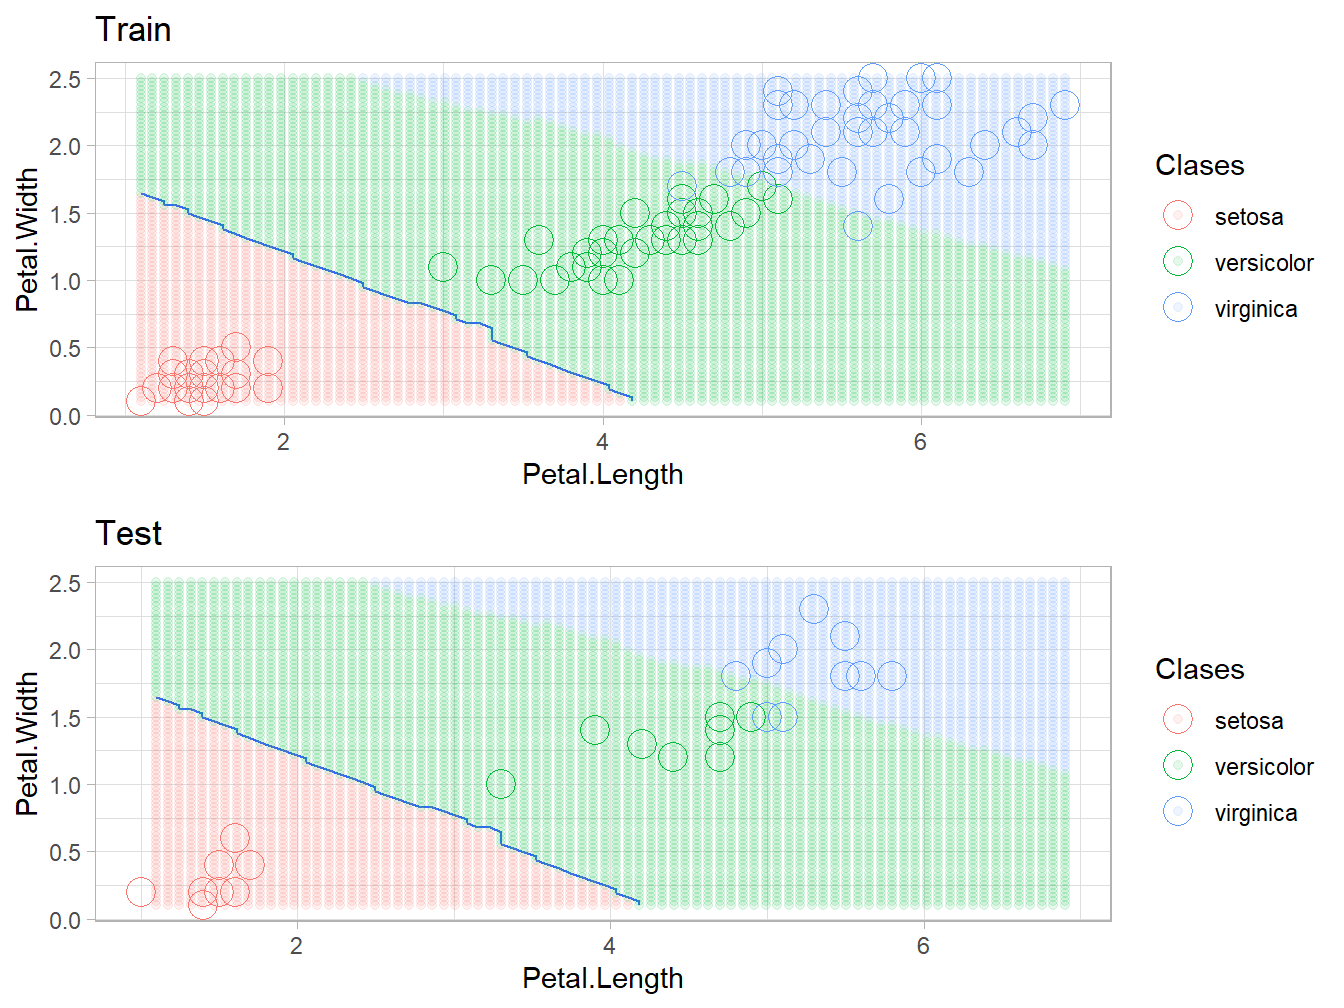
\includegraphics[width=0.8\linewidth]{_main_files/figure-latex/unnamed-chunk-21-1} \end{center}

\hypertarget{regresiuxf3n}{%
\section{Regresión}\label{regresiuxf3n}}

Abordamos ahora el problema de regresión con KNN, o sea, la respuesta es cuantitativa-continua. Seguimos usando el paquete \texttt{caret} que tiene implementado el algoritmo y ofrece facilidades para el preprocesado de los datos y la validación del modelo.

Particularmente, atacaremos el problema de predecir el precio medio de las viviendas (\texttt{medv}) en los suburbios de Boston, usando otras 13 variables predictoras.

\begin{Shaded}
\begin{Highlighting}[]
\KeywordTok{library}\NormalTok{(MASS)}
\KeywordTok{library}\NormalTok{(caret)}
\KeywordTok{library}\NormalTok{(ggplot2)}

\CommentTok{# cargar e inspeccionar los datos}
\CommentTok{# para detalles sobre las variables predictoras:}
\CommentTok{# ?Boston}
\KeywordTok{data}\NormalTok{(Boston)}
\KeywordTok{str}\NormalTok{(Boston)}
\end{Highlighting}
\end{Shaded}

\begin{verbatim}
## 'data.frame':    506 obs. of  14 variables:
##  $ crim   : num  0.00632 0.02731 0.02729 0.03237 0.06905 ...
##  $ zn     : num  18 0 0 0 0 0 12.5 12.5 12.5 12.5 ...
##  $ indus  : num  2.31 7.07 7.07 2.18 2.18 2.18 7.87 7.87 7.87 7.87 ...
##  $ chas   : int  0 0 0 0 0 0 0 0 0 0 ...
##  $ nox    : num  0.538 0.469 0.469 0.458 0.458 0.458 0.524 0.524 0.524 0.524 ...
##  $ rm     : num  6.58 6.42 7.18 7 7.15 ...
##  $ age    : num  65.2 78.9 61.1 45.8 54.2 58.7 66.6 96.1 100 85.9 ...
##  $ dis    : num  4.09 4.97 4.97 6.06 6.06 ...
##  $ rad    : int  1 2 2 3 3 3 5 5 5 5 ...
##  $ tax    : num  296 242 242 222 222 222 311 311 311 311 ...
##  $ ptratio: num  15.3 17.8 17.8 18.7 18.7 18.7 15.2 15.2 15.2 15.2 ...
##  $ black  : num  397 397 393 395 397 ...
##  $ lstat  : num  4.98 9.14 4.03 2.94 5.33 ...
##  $ medv   : num  24 21.6 34.7 33.4 36.2 28.7 22.9 27.1 16.5 18.9 ...
\end{verbatim}

\begin{Shaded}
\begin{Highlighting}[]
\KeywordTok{summary}\NormalTok{(Boston)}
\end{Highlighting}
\end{Shaded}

\begin{verbatim}
##       crim                zn             indus            chas        
##  Min.   : 0.00632   Min.   :  0.00   Min.   : 0.46   Min.   :0.00000  
##  1st Qu.: 0.08204   1st Qu.:  0.00   1st Qu.: 5.19   1st Qu.:0.00000  
##  Median : 0.25651   Median :  0.00   Median : 9.69   Median :0.00000  
##  Mean   : 3.61352   Mean   : 11.36   Mean   :11.14   Mean   :0.06917  
##  3rd Qu.: 3.67708   3rd Qu.: 12.50   3rd Qu.:18.10   3rd Qu.:0.00000  
##  Max.   :88.97620   Max.   :100.00   Max.   :27.74   Max.   :1.00000  
##       nox               rm             age              dis        
##  Min.   :0.3850   Min.   :3.561   Min.   :  2.90   Min.   : 1.130  
##  1st Qu.:0.4490   1st Qu.:5.886   1st Qu.: 45.02   1st Qu.: 2.100  
##  Median :0.5380   Median :6.208   Median : 77.50   Median : 3.207  
##  Mean   :0.5547   Mean   :6.285   Mean   : 68.57   Mean   : 3.795  
##  3rd Qu.:0.6240   3rd Qu.:6.623   3rd Qu.: 94.08   3rd Qu.: 5.188  
##  Max.   :0.8710   Max.   :8.780   Max.   :100.00   Max.   :12.127  
##       rad              tax           ptratio          black       
##  Min.   : 1.000   Min.   :187.0   Min.   :12.60   Min.   :  0.32  
##  1st Qu.: 4.000   1st Qu.:279.0   1st Qu.:17.40   1st Qu.:375.38  
##  Median : 5.000   Median :330.0   Median :19.05   Median :391.44  
##  Mean   : 9.549   Mean   :408.2   Mean   :18.46   Mean   :356.67  
##  3rd Qu.:24.000   3rd Qu.:666.0   3rd Qu.:20.20   3rd Qu.:396.23  
##  Max.   :24.000   Max.   :711.0   Max.   :22.00   Max.   :396.90  
##      lstat            medv      
##  Min.   : 1.73   Min.   : 5.00  
##  1st Qu.: 6.95   1st Qu.:17.02  
##  Median :11.36   Median :21.20  
##  Mean   :12.65   Mean   :22.53  
##  3rd Qu.:16.95   3rd Qu.:25.00  
##  Max.   :37.97   Max.   :50.00
\end{verbatim}

Veamos las relaciones entre predictores y la variable respuesta (en este ejemplo, solo hemos representado algunas).

\begin{Shaded}
\begin{Highlighting}[]
\CommentTok{# ver correlaciones y posibles relaciones:}

\CommentTok{# todos los predictores:}
\CommentTok{# ggpairs(Boston, ggplot2::aes(y = medv, alpha = 0.2)) + theme_light()}
\CommentTok{# algunos predictores:}
\KeywordTok{ggpairs}\NormalTok{(Boston[, }\KeywordTok{c}\NormalTok{(}\StringTok{"lstat"}\NormalTok{, }\StringTok{"age"}\NormalTok{, }\StringTok{"rad"}\NormalTok{, }\StringTok{"rm"}\NormalTok{, }\StringTok{"ptratio"}\NormalTok{, }\StringTok{"medv"}\NormalTok{)]) }\OperatorTok{+}\StringTok{ }\KeywordTok{theme_light}\NormalTok{()}
\end{Highlighting}
\end{Shaded}

\begin{center}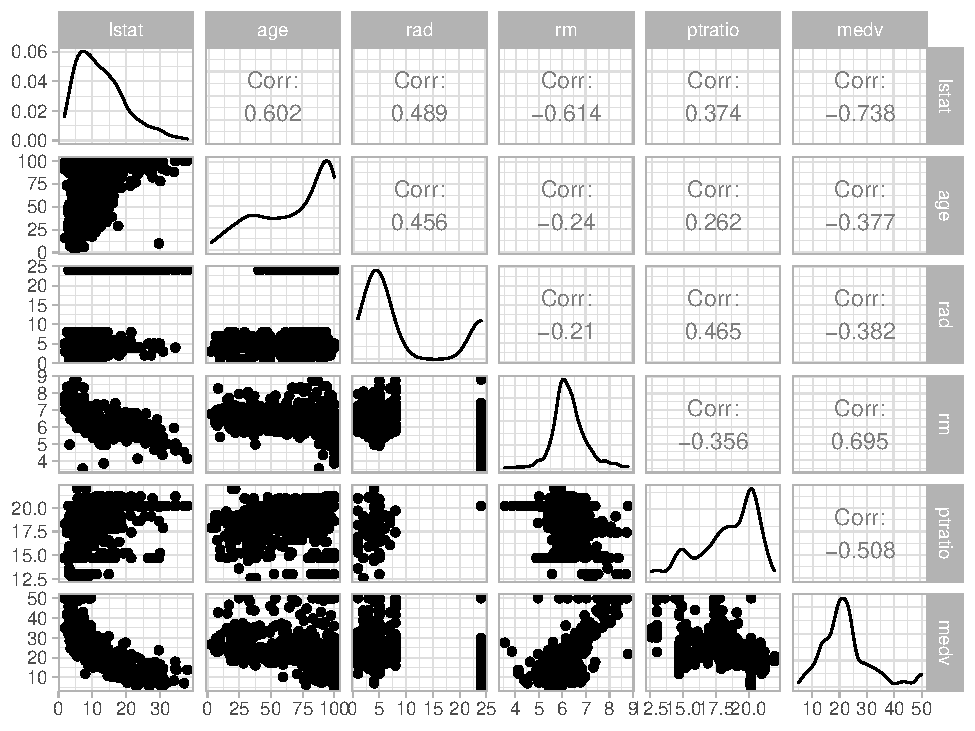
\includegraphics[width=0.8\linewidth]{_main_files/figure-latex/unnamed-chunk-23-1} \end{center}

Por ejemplo, es notable la relación lineal entre \texttt{medv} y las variables predictoras \texttt{rm} y \texttt{lstat}. Estas dos corresponden al número medio de habitaciones por vivienda y al ínfimo estatus poblacional, respectivamente.

Ajustemos un modelo de regresión, usando todas las variables y el algoritmo KNN.

\begin{Shaded}
\begin{Highlighting}[]
\CommentTok{# Split the data into training and test set}
\KeywordTok{set.seed}\NormalTok{(}\DecValTok{123}\NormalTok{)}
\NormalTok{train.ID <-}\StringTok{ }\KeywordTok{createDataPartition}\NormalTok{(Boston}\OperatorTok{$}\NormalTok{medv, }\DataTypeTok{p =} \FloatTok{0.8}\NormalTok{, }\DataTypeTok{list =} \OtherTok{FALSE}\NormalTok{)}
\NormalTok{train.data  <-}\StringTok{ }\NormalTok{Boston[train.ID, ]}
\NormalTok{test.data <-}\StringTok{ }\NormalTok{Boston[}\OperatorTok{-}\NormalTok{train.ID, ]}

\CommentTok{# Fit the model on the training set}
\KeywordTok{set.seed}\NormalTok{(}\DecValTok{123}\NormalTok{)}
\NormalTok{knn_reg_model <-}\StringTok{ }\KeywordTok{train}\NormalTok{(}
\NormalTok{  medv}\OperatorTok{~}\NormalTok{.,}
  \DataTypeTok{data =}\NormalTok{ train.data,}
  \DataTypeTok{method =} \StringTok{"knn"}\NormalTok{,}
  \DataTypeTok{trControl =} \KeywordTok{trainControl}\NormalTok{(}\StringTok{"cv"}\NormalTok{, }\DataTypeTok{number =} \DecValTok{10}\NormalTok{),}
  \DataTypeTok{preProcess =} \KeywordTok{c}\NormalTok{(}\StringTok{"center"}\NormalTok{,}\StringTok{"scale"}\NormalTok{),}
  \DataTypeTok{tuneLength =} \DecValTok{20}
\NormalTok{)}

\NormalTok{knn_reg_model}
\end{Highlighting}
\end{Shaded}

\begin{verbatim}
## k-Nearest Neighbors 
## 
## 407 samples
##  13 predictor
## 
## Pre-processing: centered (13), scaled (13) 
## Resampling: Cross-Validated (10 fold) 
## Summary of sample sizes: 366, 367, 366, 366, 366, 366, ... 
## Resampling results across tuning parameters:
## 
##   k   RMSE      Rsquared   MAE     
##    5  4.446665  0.7748420  2.877705
##    7  4.513433  0.7760351  2.931696
##    9  4.510659  0.7822810  2.961313
##   11  4.557329  0.7806128  2.997708
##   13  4.589419  0.7769459  3.031409
##   15  4.683314  0.7715242  3.108591
##   17  4.727456  0.7658943  3.133048
##   19  4.794512  0.7608152  3.190837
##   21  4.871432  0.7555146  3.242578
##   23  4.896989  0.7568145  3.256753
##   25  4.982893  0.7505900  3.318786
##   27  5.035171  0.7497412  3.356345
##   29  5.099070  0.7472969  3.412470
##   31  5.196655  0.7375974  3.477003
##   33  5.260674  0.7329066  3.507057
##   35  5.320022  0.7310458  3.543261
##   37  5.393032  0.7258230  3.592311
##   39  5.457338  0.7205076  3.643305
##   41  5.500014  0.7178285  3.669332
##   43  5.561854  0.7125909  3.713330
## 
## RMSE was used to select the optimal model using the smallest value.
## The final value used for the model was k = 5.
\end{verbatim}

\begin{Shaded}
\begin{Highlighting}[]
\CommentTok{# Plot model error RMSE vs different values of k}
\KeywordTok{plot}\NormalTok{(knn_reg_model)}
\end{Highlighting}
\end{Shaded}

\begin{center}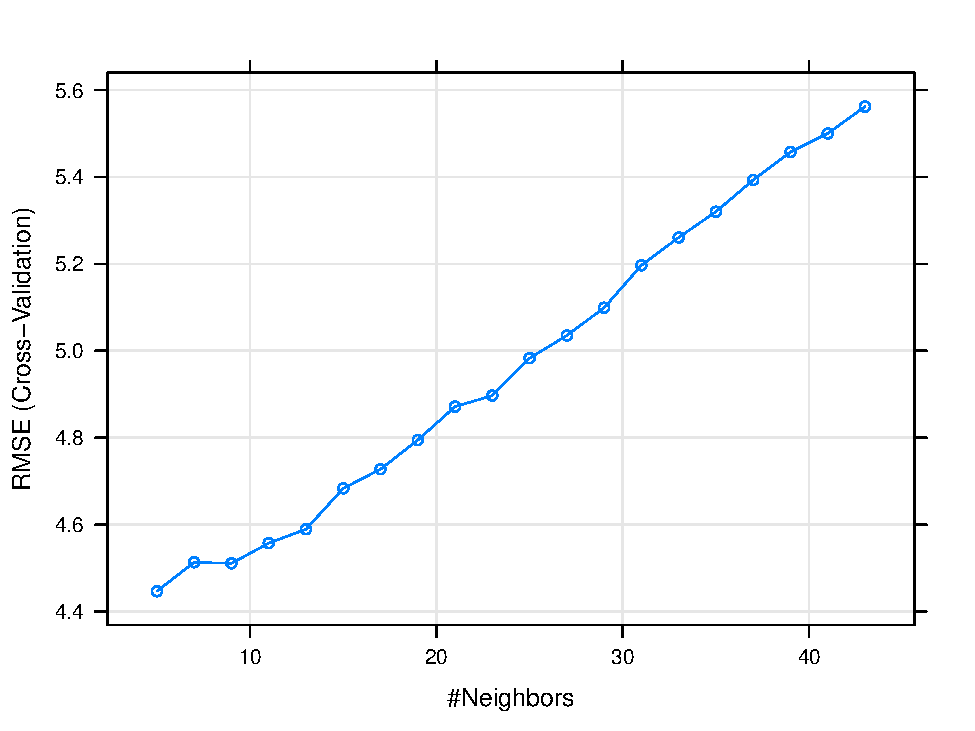
\includegraphics[width=0.8\linewidth]{_main_files/figure-latex/unnamed-chunk-24-1} \end{center}

Ahora, lo que nos interesa es disminuir el Error Cuadrático Medio:

\begin{Shaded}
\begin{Highlighting}[]
\CommentTok{# predicciones}
\NormalTok{predictions <-}\StringTok{ }\KeywordTok{predict}\NormalTok{(knn_reg_model, test.data)}
\CommentTok{# RMSE: raíz del error cuadrático medio}
\KeywordTok{RMSE}\NormalTok{(predictions, test.data}\OperatorTok{$}\NormalTok{medv)}
\end{Highlighting}
\end{Shaded}

\begin{verbatim}
## [1] 4.762122
\end{verbatim}

\begin{Shaded}
\begin{Highlighting}[]
\CommentTok{# MAE: error absoluto medio}
\KeywordTok{MAE}\NormalTok{(predictions, test.data}\OperatorTok{$}\NormalTok{medv)}
\end{Highlighting}
\end{Shaded}

\begin{verbatim}
## [1] 3.050101
\end{verbatim}

Si representamos las predicciones y los valores reales de la variable \texttt{medv}, esperamos que los puntos estén muy cercanos a la recta \(Y = X\).

\begin{Shaded}
\begin{Highlighting}[]
\NormalTok{df_plot <-}\StringTok{ }\KeywordTok{data.frame}\NormalTok{(}\DataTypeTok{pred =}\NormalTok{ predictions, }\DataTypeTok{real =}\NormalTok{ test.data}\OperatorTok{$}\NormalTok{medv)}
\KeywordTok{ggplot}\NormalTok{(df_plot, }\KeywordTok{aes}\NormalTok{(}\DataTypeTok{x =}\NormalTok{ pred, }\DataTypeTok{y =}\NormalTok{ real)) }\OperatorTok{+}
\StringTok{  }\KeywordTok{geom_point}\NormalTok{() }\OperatorTok{+}
\StringTok{  }\KeywordTok{geom_abline}\NormalTok{(}\DataTypeTok{slope =} \DecValTok{1}\NormalTok{, }\DataTypeTok{intercept =} \DecValTok{0}\NormalTok{) }\OperatorTok{+}
\StringTok{  }\KeywordTok{xlab}\NormalTok{(}\KeywordTok{expression}\NormalTok{(}\KeywordTok{hat}\NormalTok{( y))) }\OperatorTok{+}\StringTok{ }\KeywordTok{ylab}\NormalTok{(}\StringTok{"y"}\NormalTok{) }\OperatorTok{+}
\StringTok{  }\KeywordTok{theme_light}\NormalTok{()}
\end{Highlighting}
\end{Shaded}

\begin{center}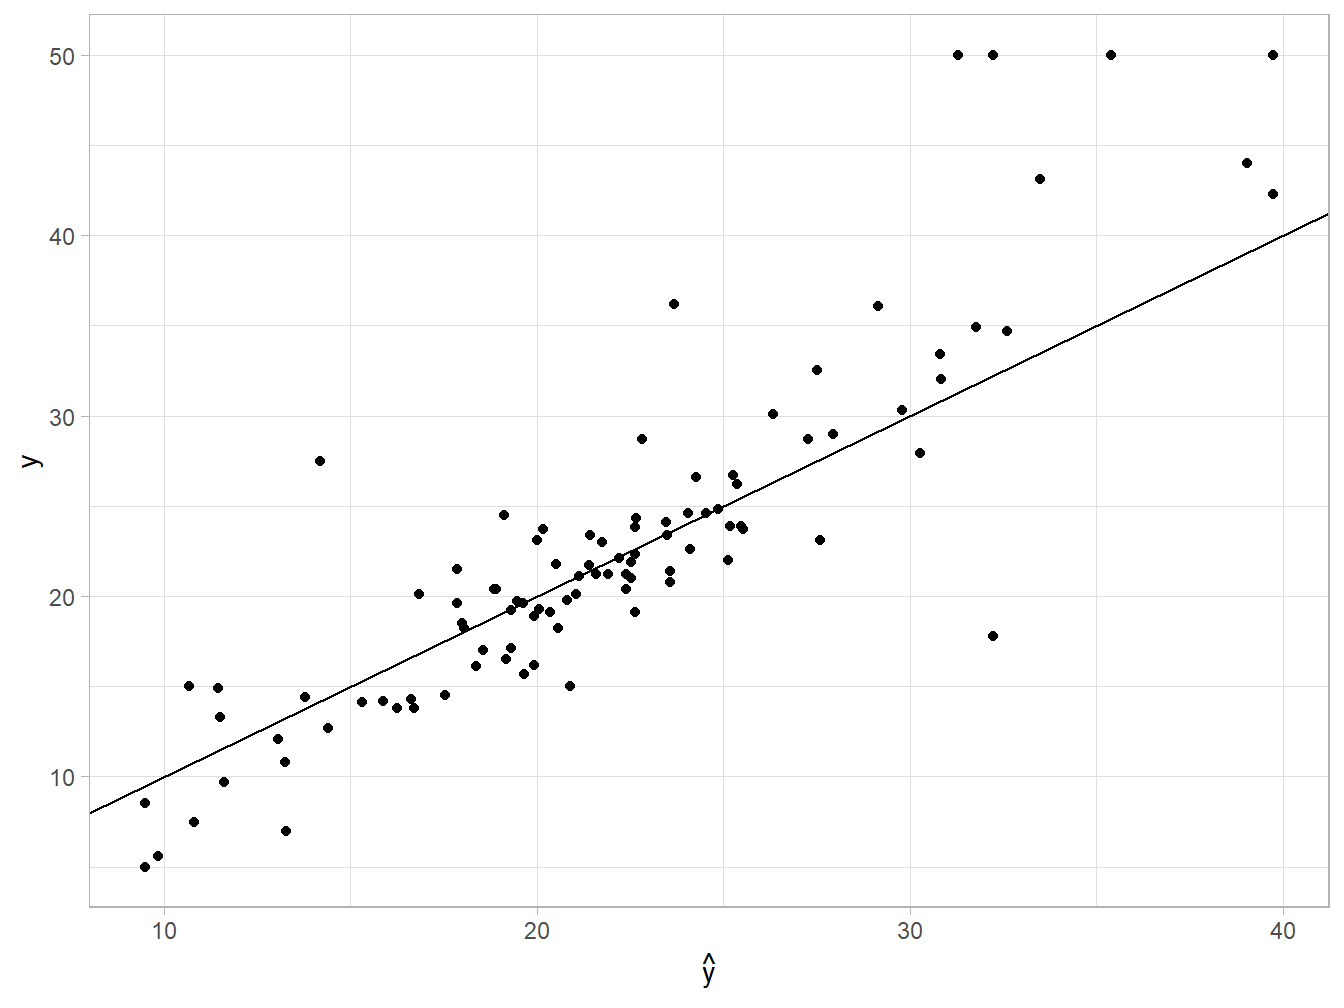
\includegraphics[width=0.8\linewidth]{_main_files/figure-latex/unnamed-chunk-26-1} \end{center}

¿Será posible mejorar esto? ¿Son todas las variables realmente necesarias? ¿Un grid con valores más pequeños a \(K = 5\) podría resultar mejor? Veamos qué tal es el ajuste y las predicciones si nos limitamos a unas pocas variables predictoras.

\begin{Shaded}
\begin{Highlighting}[]
\CommentTok{# importancia de las variables según impacto en la predicción}
\KeywordTok{varImp}\NormalTok{(knn_reg_model)}
\end{Highlighting}
\end{Shaded}

\begin{verbatim}
## loess r-squared variable importance
## 
##         Overall
## lstat    100.00
## rm        84.11
## ptratio   35.71
## indus     33.76
## crim      30.80
## tax       30.16
## black     25.33
## nox       24.24
## age       21.19
## rad       18.94
## dis       15.00
## zn        14.23
## chas       0.00
\end{verbatim}

\begin{Shaded}
\begin{Highlighting}[]
\CommentTok{# seleccionemos solo algunas variables:}
\NormalTok{boston <-}\StringTok{ }\NormalTok{Boston[, }\KeywordTok{c}\NormalTok{(}\StringTok{"lstat"}\NormalTok{, }\StringTok{"rm"}\NormalTok{, }\StringTok{"ptratio"}\NormalTok{, }\StringTok{"medv"}\NormalTok{)]}
\end{Highlighting}
\end{Shaded}

\begin{Shaded}
\begin{Highlighting}[]
\CommentTok{# ajustamos el modelo en el nuevo diseño}
\NormalTok{train.data  <-}\StringTok{ }\NormalTok{boston[train.ID, ]}
\NormalTok{test.data <-}\StringTok{ }\NormalTok{boston[}\OperatorTok{-}\NormalTok{train.ID, ]}

\KeywordTok{set.seed}\NormalTok{(}\DecValTok{123}\NormalTok{)}
\NormalTok{knn_reg_model <-}\StringTok{ }\KeywordTok{train}\NormalTok{(}
\NormalTok{  medv}\OperatorTok{~}\NormalTok{.,}
  \DataTypeTok{data =}\NormalTok{ train.data,}
  \DataTypeTok{method =} \StringTok{"knn"}\NormalTok{,}
  \DataTypeTok{trControl =} \KeywordTok{trainControl}\NormalTok{(}\StringTok{"cv"}\NormalTok{, }\DataTypeTok{number =} \DecValTok{10}\NormalTok{),}
  \DataTypeTok{preProcess =} \KeywordTok{c}\NormalTok{(}\StringTok{"center"}\NormalTok{,}\StringTok{"scale"}\NormalTok{),}
  \DataTypeTok{tuneGrid =} \KeywordTok{expand.grid}\NormalTok{(}\DataTypeTok{k =} \DecValTok{1}\OperatorTok{:}\DecValTok{15}\NormalTok{)}
\NormalTok{)}

\CommentTok{# Veamos si el modelo ha mejorado algo:}

\CommentTok{# predicciones}
\NormalTok{predictions <-}\StringTok{ }\KeywordTok{predict}\NormalTok{(knn_reg_model, test.data)}
\CommentTok{# RMSE: raíz del error cuadrático medio}
\KeywordTok{RMSE}\NormalTok{(predictions, test.data}\OperatorTok{$}\NormalTok{medv)}
\end{Highlighting}
\end{Shaded}

\begin{verbatim}
## [1] 4.33752
\end{verbatim}

\begin{Shaded}
\begin{Highlighting}[]
\CommentTok{# MAE: error absoluto medio}
\KeywordTok{MAE}\NormalTok{(predictions, test.data}\OperatorTok{$}\NormalTok{medv)}
\end{Highlighting}
\end{Shaded}

\begin{verbatim}
## [1] 2.805195
\end{verbatim}

\begin{Shaded}
\begin{Highlighting}[]
\NormalTok{df_plot <-}\StringTok{ }\KeywordTok{data.frame}\NormalTok{(}\DataTypeTok{pred =}\NormalTok{ predictions, }\DataTypeTok{real =}\NormalTok{ test.data}\OperatorTok{$}\NormalTok{medv)}
\KeywordTok{ggplot}\NormalTok{(df_plot, }\KeywordTok{aes}\NormalTok{(}\DataTypeTok{x =}\NormalTok{ pred, }\DataTypeTok{y =}\NormalTok{ real)) }\OperatorTok{+}
\StringTok{  }\KeywordTok{geom_point}\NormalTok{() }\OperatorTok{+}
\StringTok{  }\KeywordTok{geom_abline}\NormalTok{(}\DataTypeTok{slope =} \DecValTok{1}\NormalTok{, }\DataTypeTok{intercept =} \DecValTok{0}\NormalTok{) }\OperatorTok{+}
\StringTok{  }\KeywordTok{xlab}\NormalTok{(}\KeywordTok{expression}\NormalTok{(}\KeywordTok{hat}\NormalTok{( y))) }\OperatorTok{+}\StringTok{ }\KeywordTok{ylab}\NormalTok{(}\StringTok{"y"}\NormalTok{) }\OperatorTok{+}
\StringTok{  }\KeywordTok{theme_light}\NormalTok{()}
\end{Highlighting}
\end{Shaded}

\begin{center}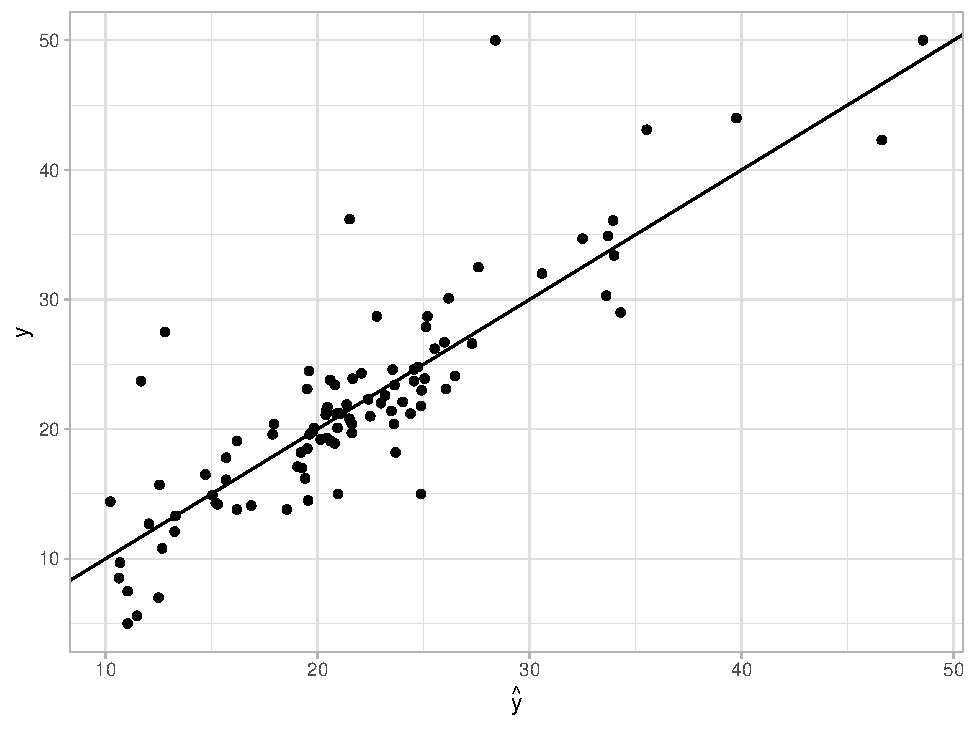
\includegraphics[width=0.8\linewidth]{_main_files/figure-latex/unnamed-chunk-29-1} \end{center}

\hypertarget{weighted-knn}{%
\section{Weighted KNN}\label{weighted-knn}}

El método de K-Vecinos Más Próximos Ponderados (WKNN: \emph{Weighted K-Nearest Neighbors}) es una variante del KNN. El principio básico es el mismo: predecir una respuesta en función de los puntos más cercanos de la muestra. La diferencia es que WKNN da más importancia a los más próximos, dentro de los K prefijados. Esto se logra ponderando o dando pesos a los vecinos.

En \texttt{caret} podemos fijar el método \texttt{kknn} que implementa WKNN, tanto para regresión como para clasificación. Ahora debemos optimizar 3 hiperparámetros:

\begin{Shaded}
\begin{Highlighting}[]
\KeywordTok{getModelInfo}\NormalTok{(}\StringTok{"kknn"}\NormalTok{)}\OperatorTok{$}\NormalTok{kknn}\OperatorTok{$}\NormalTok{parameters}
\end{Highlighting}
\end{Shaded}

\begin{verbatim}
##   parameter     class           label
## 1      kmax   numeric Max. #Neighbors
## 2  distance   numeric        Distance
## 3    kernel character          Kernel
\end{verbatim}

El número de vecinos \texttt{K} se corresponde al campo\texttt{kmax}. El campo \texttt{distance} se refiere al order del parámetro \(p\) en la \emph{Distancia de Minkowski}. El \texttt{kernel} es la transformación de los ejes de coordenadas, las opciones son:

\begin{Shaded}
\begin{Highlighting}[]
\NormalTok{kerns <-}\StringTok{ }\KeywordTok{c}\NormalTok{(}\StringTok{"rectangular"}\NormalTok{, }\StringTok{"triangular"}\NormalTok{, }\StringTok{"epanechnikov"}\NormalTok{, }\StringTok{"biweight"}\NormalTok{, }\StringTok{"triweight"}\NormalTok{, }
                                 \StringTok{"cos"}\NormalTok{, }\StringTok{"inv"}\NormalTok{, }\StringTok{"gaussian"}\NormalTok{)}
\end{Highlighting}
\end{Shaded}

Veamos un ejemplo con los datos \texttt{iris}. Empezamos fijando un grid o malla de posibles valores de los hiperparámetros a optimizar:

\begin{Shaded}
\begin{Highlighting}[]
\CommentTok{# muestra, por eso es necesario una particion balanceada con createDataPartition}
\NormalTok{df <-}\StringTok{ }\NormalTok{iris}
\KeywordTok{set.seed}\NormalTok{(}\DecValTok{123}\NormalTok{)}
\NormalTok{train.ID <-}\StringTok{ }\KeywordTok{createDataPartition}\NormalTok{(df}\OperatorTok{$}\NormalTok{Species, }\DataTypeTok{p =} \FloatTok{0.8}\NormalTok{, }\DataTypeTok{list =} \OtherTok{FALSE}\NormalTok{)}

\NormalTok{train_df <-}\StringTok{ }\NormalTok{df[train.ID, ]}
\NormalTok{test_df <-}\StringTok{ }\NormalTok{df[}\OperatorTok{-}\NormalTok{train.ID, ]}

\CommentTok{# hacemos una validación cruzada con 10-folds 10 veces}
\NormalTok{fit_control <-}\StringTok{ }\KeywordTok{trainControl}\NormalTok{(}\DataTypeTok{method=}\StringTok{'repeatedcv'}\NormalTok{, }\DataTypeTok{number =} \DecValTok{10}\NormalTok{, }\DataTypeTok{repeats =} \DecValTok{10}\NormalTok{)}

\CommentTok{# fijamos el grid de valores de los hiperparámetros:}
\NormalTok{buscar_mejor <-}\StringTok{ }\KeywordTok{expand.grid}\NormalTok{( }\DataTypeTok{kmax =}  \DecValTok{3}\OperatorTok{:}\DecValTok{9}\NormalTok{,}
                             \DataTypeTok{distance =} \DecValTok{1}\OperatorTok{:}\DecValTok{2}\NormalTok{,}
                             \DataTypeTok{kernel =} \KeywordTok{c}\NormalTok{(}\StringTok{"rectangular"}\NormalTok{, }\CommentTok{#standard knn}
                                        \StringTok{"triangular"}\NormalTok{,}
                                        \StringTok{"gaussian"}\NormalTok{))}
\end{Highlighting}
\end{Shaded}

El modelo se ajusta igual a como ya hemos estudiado:

\begin{Shaded}
\begin{Highlighting}[]
\KeywordTok{set.seed}\NormalTok{(}\DecValTok{321}\NormalTok{)}
\NormalTok{model.w.knn <-}\StringTok{ }\KeywordTok{train}\NormalTok{(Species }\OperatorTok{~}\NormalTok{.,}
                     \DataTypeTok{data =}\NormalTok{ train_df,}
                     \DataTypeTok{method =} \StringTok{"kknn"}\NormalTok{,}
                     \DataTypeTok{trControl =}\NormalTok{ fit_control,}
                     \DataTypeTok{preProcess =} \KeywordTok{c}\NormalTok{(}\StringTok{"center"}\NormalTok{, }\StringTok{"scale"}\NormalTok{),}
                     \DataTypeTok{tuneGrid =}\NormalTok{ buscar_mejor)}
\NormalTok{model.w.knn}
\end{Highlighting}
\end{Shaded}

\begin{verbatim}
## k-Nearest Neighbors 
## 
## 120 samples
##   4 predictor
##   3 classes: 'setosa', 'versicolor', 'virginica' 
## 
## Pre-processing: centered (4), scaled (4) 
## Resampling: Cross-Validated (10 fold, repeated 10 times) 
## Summary of sample sizes: 108, 108, 108, 108, 108, 108, ... 
## Resampling results across tuning parameters:
## 
##   kmax  distance  kernel       Accuracy   Kappa  
##   3     1         rectangular  0.9600000  0.94000
##   3     1         triangular   0.9558333  0.93375
##   3     1         gaussian     0.9583333  0.93750
##   3     2         rectangular  0.9508333  0.92625
##   3     2         triangular   0.9550000  0.93250
##   3     2         gaussian     0.9483333  0.92250
##   4     1         rectangular  0.9600000  0.94000
##   4     1         triangular   0.9558333  0.93375
##   4     1         gaussian     0.9583333  0.93750
##   4     2         rectangular  0.9491667  0.92375
##   4     2         triangular   0.9550000  0.93250
##   4     2         gaussian     0.9458333  0.91875
##   5     1         rectangular  0.9575000  0.93625
##   5     1         triangular   0.9558333  0.93375
##   5     1         gaussian     0.9583333  0.93750
##   5     2         rectangular  0.9400000  0.91000
##   5     2         triangular   0.9566667  0.93500
##   5     2         gaussian     0.9591667  0.93875
##   6     1         rectangular  0.9575000  0.93625
##   6     1         triangular   0.9558333  0.93375
##   6     1         gaussian     0.9550000  0.93250
##   6     2         rectangular  0.9416667  0.91250
##   6     2         triangular   0.9558333  0.93375
##   6     2         gaussian     0.9558333  0.93375
##   7     1         rectangular  0.9550000  0.93250
##   7     1         triangular   0.9558333  0.93375
##   7     1         gaussian     0.9558333  0.93375
##   7     2         rectangular  0.9433333  0.91500
##   7     2         triangular   0.9575000  0.93625
##   7     2         gaussian     0.9558333  0.93375
##   8     1         rectangular  0.9550000  0.93250
##   8     1         triangular   0.9558333  0.93375
##   8     1         gaussian     0.9558333  0.93375
##   8     2         rectangular  0.9433333  0.91500
##   8     2         triangular   0.9616667  0.94250
##   8     2         gaussian     0.9583333  0.93750
##   9     1         rectangular  0.9550000  0.93250
##   9     1         triangular   0.9558333  0.93375
##   9     1         gaussian     0.9558333  0.93375
##   9     2         rectangular  0.9450000  0.91750
##   9     2         triangular   0.9675000  0.95125
##   9     2         gaussian     0.9608333  0.94125
## 
## Accuracy was used to select the optimal model using the largest value.
## The final values used for the model were kmax = 9, distance = 2 and kernel
##  = triangular.
\end{verbatim}

\begin{Shaded}
\begin{Highlighting}[]
\NormalTok{model.w.knn}\OperatorTok{$}\NormalTok{finalModel}
\end{Highlighting}
\end{Shaded}

\begin{verbatim}
## 
## Call:
## kknn::train.kknn(formula = .outcome ~ ., data = dat, kmax = param$kmax,     distance = param$distance, kernel = as.character(param$kernel))
## 
## Type of response variable: nominal
## Minimal misclassification: 0.01666667
## Best kernel: triangular
## Best k: 9
\end{verbatim}

\begin{Shaded}
\begin{Highlighting}[]
\KeywordTok{plot}\NormalTok{(model.w.knn)}
\end{Highlighting}
\end{Shaded}

\begin{center}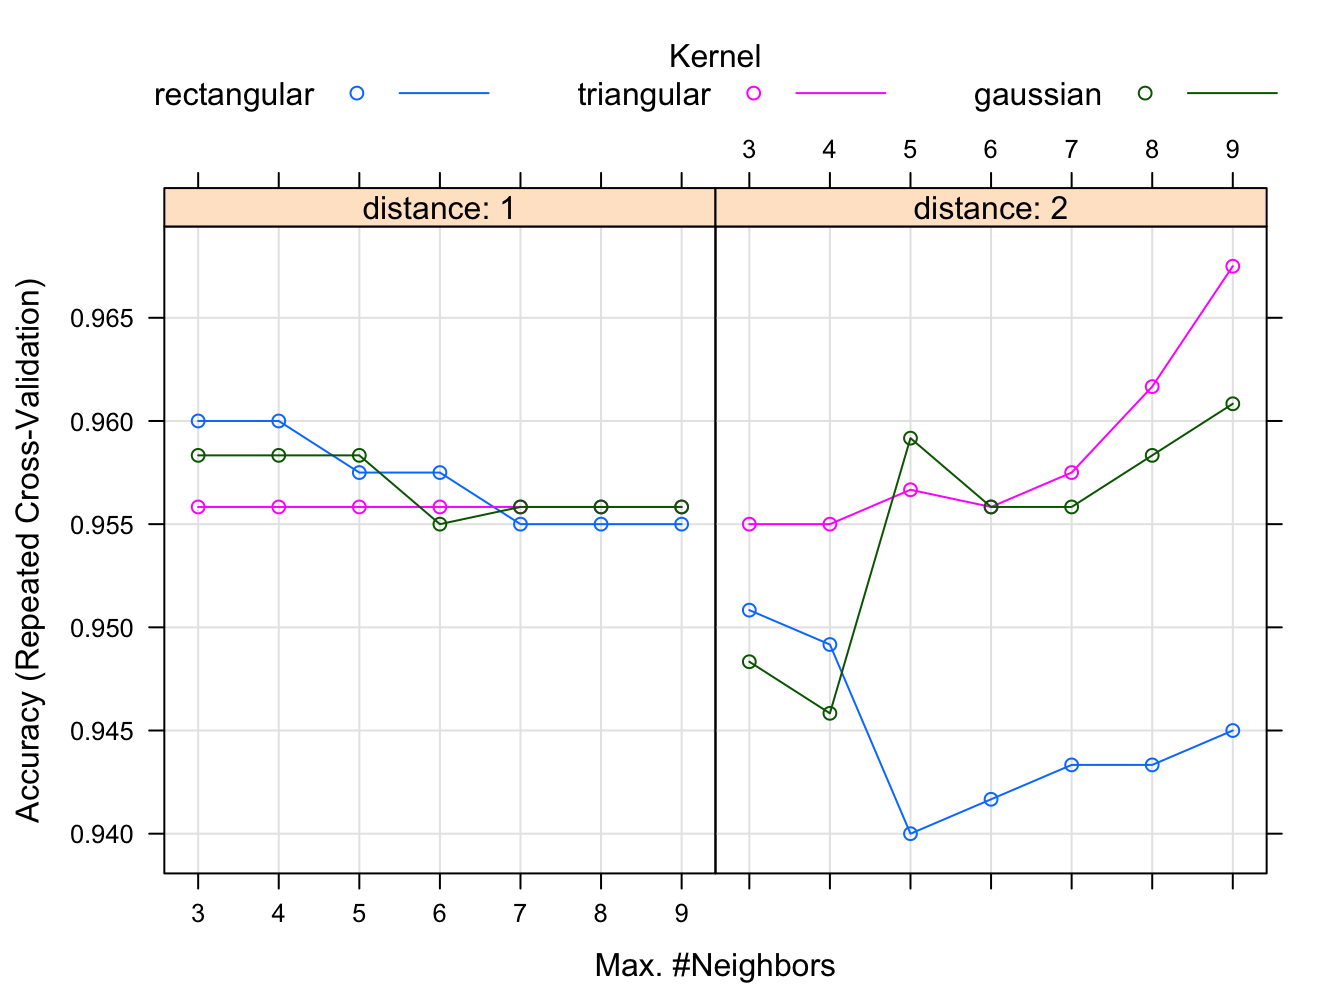
\includegraphics[width=0.8\linewidth]{_main_files/figure-latex/unnamed-chunk-34-1} \end{center}

Observamos que el modelo final, el mejor de acuerdo al \texttt{Accuracy} es aquel con 8 vecinos, donde el parámetro \(p=2\) en la Distancia de Minkowski (esto es equivalente a la Distancia Euclídea) y el kernel es triangular. Por otro lado, en lugar de escribir explícitamente el grid de valores a probar, en \texttt{caret} tenemos la opción de realizar una búsqueda aleatoria. Esto podría ser un primer paso para detectar rangos de valores de los hiperparámetros donde luego afinar la búsqueda. Como ejemplo, lo haremos para solo 8 combinaciones de posibles hiperparámetros (en la práctica debemos fijar un mayor número de combinaciones, lo que conlleva un mayor coste computacional):

\begin{Shaded}
\begin{Highlighting}[]
\CommentTok{# random search WKNN}
\NormalTok{fit_control <-}\StringTok{ }\KeywordTok{trainControl}\NormalTok{(}\DataTypeTok{method=}\StringTok{'repeatedcv'}\NormalTok{, }\DataTypeTok{number =} \DecValTok{10}\NormalTok{, }
                            \DataTypeTok{repeats =} \DecValTok{10}\NormalTok{,}
                            \DataTypeTok{search =} \StringTok{"random"}\NormalTok{)}
\KeywordTok{set.seed}\NormalTok{(}\DecValTok{321}\NormalTok{)}
\NormalTok{model.w.knn <-}\StringTok{ }\KeywordTok{train}\NormalTok{(Species }\OperatorTok{~}\NormalTok{.,}
                     \DataTypeTok{data =}\NormalTok{ train_df,}
                     \DataTypeTok{method =} \StringTok{"kknn"}\NormalTok{,}
                     \DataTypeTok{trControl =}\NormalTok{ fit_control,}
                     \DataTypeTok{preProcess =} \KeywordTok{c}\NormalTok{(}\StringTok{"center"}\NormalTok{, }\StringTok{"scale"}\NormalTok{),}
                     \DataTypeTok{tuneLength =} \DecValTok{8}\NormalTok{)}
\NormalTok{model.w.knn}
\end{Highlighting}
\end{Shaded}

\begin{verbatim}
## k-Nearest Neighbors 
## 
## 120 samples
##   4 predictor
##   3 classes: 'setosa', 'versicolor', 'virginica' 
## 
## Pre-processing: centered (4), scaled (4) 
## Resampling: Cross-Validated (10 fold, repeated 10 times) 
## Summary of sample sizes: 108, 108, 108, 108, 108, 108, ... 
## Resampling results across tuning parameters:
## 
##   kmax  distance   kernel        Accuracy   Kappa  
##    1    0.8715102  biweight      0.9566667  0.93500
##   10    1.9213770  cos           0.9658333  0.94875
##   22    0.6048966  epanechnikov  0.9541667  0.93125
##   25    1.7765156  triangular    0.9683333  0.95250
##   28    1.8982141  inv           0.9666667  0.95000
##   37    0.1352608  rectangular   0.9491667  0.92375
##   37    2.2990154  inv           0.9725000  0.95875
##   40    1.2107700  triangular    0.9583333  0.93750
## 
## Accuracy was used to select the optimal model using the largest value.
## The final values used for the model were kmax = 37, distance = 2.299015
##  and kernel = inv.
\end{verbatim}

\begin{Shaded}
\begin{Highlighting}[]
\KeywordTok{plot}\NormalTok{(model.w.knn)}
\end{Highlighting}
\end{Shaded}

\begin{center}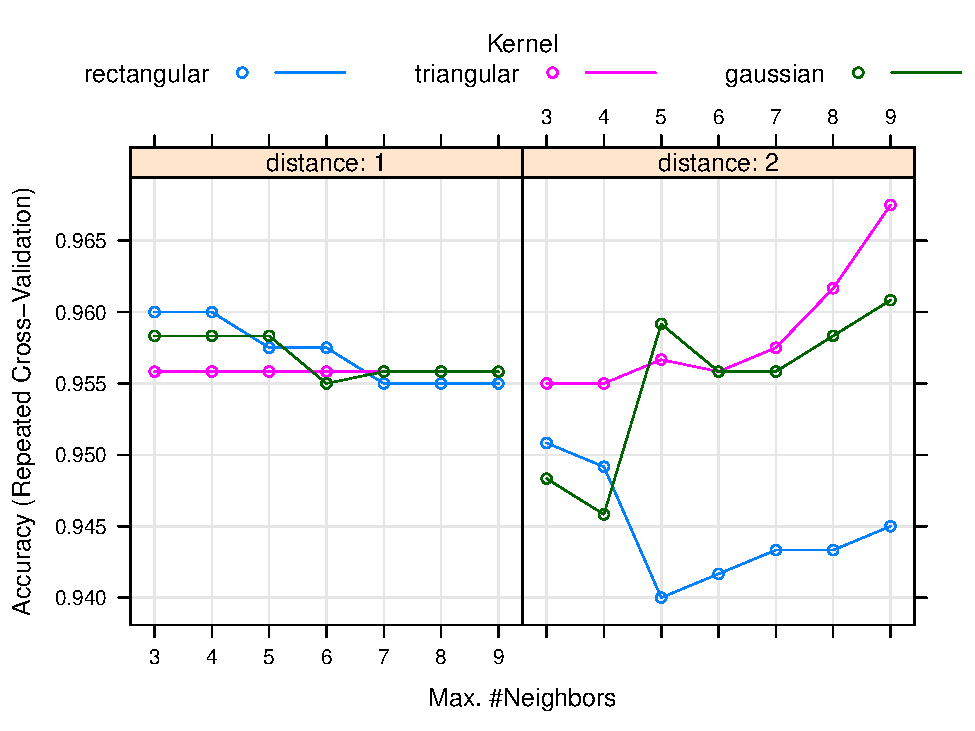
\includegraphics[width=0.8\linewidth]{_main_files/figure-latex/unnamed-chunk-35-1} \end{center}

\hypertarget{DA}{%
\chapter{Análisis Discriminante}\label{DA}}

En esta sección nos concentramos en el problema de clasificación. Particularmente, estudiaremos los métodos de \emph{Análisis Discriminante Lineal (LDA)}, \emph{Cuadrático (QDA)} y \emph{Regularizado (RDA)}. Usaremos el conjunto de datos \texttt{Default} del paquete \texttt{ISLR}:

\begin{Shaded}
\begin{Highlighting}[]
\KeywordTok{library}\NormalTok{(caret)}
\KeywordTok{library}\NormalTok{(ISLR)}

\KeywordTok{data}\NormalTok{(}\StringTok{"Default"}\NormalTok{)}
\KeywordTok{head}\NormalTok{(Default, }\DecValTok{10}\NormalTok{)}
\end{Highlighting}
\end{Shaded}

\begin{verbatim}
##    default student   balance    income
## 1       No      No  729.5265 44361.625
## 2       No     Yes  817.1804 12106.135
## 3       No      No 1073.5492 31767.139
## 4       No      No  529.2506 35704.494
## 5       No      No  785.6559 38463.496
## 6       No     Yes  919.5885  7491.559
## 7       No      No  825.5133 24905.227
## 8       No     Yes  808.6675 17600.451
## 9       No      No 1161.0579 37468.529
## 10      No      No    0.0000 29275.268
\end{verbatim}

\begin{Shaded}
\begin{Highlighting}[]
\KeywordTok{str}\NormalTok{(Default)}
\end{Highlighting}
\end{Shaded}

\begin{verbatim}
## 'data.frame':    10000 obs. of  4 variables:
##  $ default: Factor w/ 2 levels "No","Yes": 1 1 1 1 1 1 1 1 1 1 ...
##  $ student: Factor w/ 2 levels "No","Yes": 1 2 1 1 1 2 1 2 1 1 ...
##  $ balance: num  730 817 1074 529 786 ...
##  $ income : num  44362 12106 31767 35704 38463 ...
\end{verbatim}

El objetivo es predecir si un sujeto de la muestre fallará en el pago de su tarjeta de crédito. Por tanto, la variable respuesta es \texttt{default}, categórica con solo los niveles \texttt{Yes} y \texttt{No}. Tenemos información sobre el balance mensual de crédito en \texttt{balance}, el salario anual en \texttt{income} y si es estudiante o no en \texttt{student}. Solo un \(3\%\) de la muestra (\(n = 10000\)), así que es una muestra muy desbalanceada.

\begin{Shaded}
\begin{Highlighting}[]
\KeywordTok{summary}\NormalTok{(Default)}
\end{Highlighting}
\end{Shaded}

\begin{verbatim}
##  default    student       balance           income     
##  No :9667   No :7056   Min.   :   0.0   Min.   :  772  
##  Yes: 333   Yes:2944   1st Qu.: 481.7   1st Qu.:21340  
##                        Median : 823.6   Median :34553  
##                        Mean   : 835.4   Mean   :33517  
##                        3rd Qu.:1166.3   3rd Qu.:43808  
##                        Max.   :2654.3   Max.   :73554
\end{verbatim}

\begin{Shaded}
\begin{Highlighting}[]
\CommentTok{# ver el balance de la muestra}
\KeywordTok{prop.table}\NormalTok{(}\KeywordTok{table}\NormalTok{(Default}\OperatorTok{$}\NormalTok{default))}
\end{Highlighting}
\end{Shaded}

\begin{verbatim}
## 
##     No    Yes 
## 0.9667 0.0333
\end{verbatim}

Nos concentramos en predecir \texttt{default} a partir de las variables predictoras \texttt{balance} e \texttt{income}. En el siguiente diagrama de dispersión se observa cierto solapamiento entre las clases a predecir, pero una clara diferenciación de acuerdo a la variable \texttt{balance}.

\begin{Shaded}
\begin{Highlighting}[]
\KeywordTok{library}\NormalTok{(ggplot2)}
\KeywordTok{library}\NormalTok{(gridExtra)}

\CommentTok{## Scatter plot con densidades ----}
\NormalTok{plot}\FloatTok{.2}\NormalTok{d <-}\StringTok{ }\KeywordTok{ggplot}\NormalTok{(Default, }\KeywordTok{aes}\NormalTok{(}\DataTypeTok{x =}\NormalTok{ balance, }\DataTypeTok{y =}\NormalTok{ income, }\DataTypeTok{group =}\NormalTok{ default)) }\OperatorTok{+}
\StringTok{  }\KeywordTok{geom_point}\NormalTok{(}\KeywordTok{aes}\NormalTok{(}\DataTypeTok{shape =}\NormalTok{ default, }\DataTypeTok{color =}\NormalTok{ default), }\DataTypeTok{alpha =} \FloatTok{0.5}\NormalTok{) }\OperatorTok{+}
\StringTok{  }\KeywordTok{theme_light}\NormalTok{()}

\CommentTok{# Empty plot}
\NormalTok{empty <-}\StringTok{ }\KeywordTok{ggplot}\NormalTok{()}\OperatorTok{+}\KeywordTok{geom_point}\NormalTok{(}\KeywordTok{aes}\NormalTok{(}\DecValTok{1}\NormalTok{,}\DecValTok{1}\NormalTok{), }\DataTypeTok{color=}\StringTok{"white"}\NormalTok{) }\OperatorTok{+}
\StringTok{  }\KeywordTok{theme}\NormalTok{(}
    \DataTypeTok{plot.background =} \KeywordTok{element_blank}\NormalTok{(),}
    \DataTypeTok{panel.grid.major =} \KeywordTok{element_blank}\NormalTok{(),}
    \DataTypeTok{panel.grid.minor =} \KeywordTok{element_blank}\NormalTok{(),}
    \DataTypeTok{panel.border =} \KeywordTok{element_blank}\NormalTok{(),}
    \DataTypeTok{panel.background =} \KeywordTok{element_blank}\NormalTok{(),}
    \DataTypeTok{axis.title.x =} \KeywordTok{element_blank}\NormalTok{(),}
    \DataTypeTok{axis.title.y =} \KeywordTok{element_blank}\NormalTok{(),}
    \DataTypeTok{axis.text.x =} \KeywordTok{element_blank}\NormalTok{(),}
    \DataTypeTok{axis.text.y =} \KeywordTok{element_blank}\NormalTok{(),}
    \DataTypeTok{axis.ticks =} \KeywordTok{element_blank}\NormalTok{()}
\NormalTok{  )}
\CommentTok{# arriba}
\NormalTok{dens.balance <-}\StringTok{ }\KeywordTok{ggplot}\NormalTok{(Default, }\KeywordTok{aes}\NormalTok{(}\DataTypeTok{x =}\NormalTok{ balance, }\DataTypeTok{group =}\NormalTok{ default)) }\OperatorTok{+}
\StringTok{  }\KeywordTok{geom_density}\NormalTok{(}\KeywordTok{aes}\NormalTok{(}\DataTypeTok{color =}\NormalTok{ default, }\DataTypeTok{fill =}\NormalTok{ default), }\DataTypeTok{alpha =} \FloatTok{0.2}\NormalTok{) }\OperatorTok{+}
\StringTok{  }\KeywordTok{theme_light}\NormalTok{()}\OperatorTok{+}
\StringTok{  }\KeywordTok{theme}\NormalTok{(}\DataTypeTok{legend.position =} \StringTok{"none"}\NormalTok{)}
\CommentTok{# derecha}
\NormalTok{dens.income <-}\StringTok{ }\KeywordTok{ggplot}\NormalTok{(Default, }\KeywordTok{aes}\NormalTok{(}\DataTypeTok{x =}\NormalTok{ income, }\DataTypeTok{group =}\NormalTok{ default)) }\OperatorTok{+}
\StringTok{  }\KeywordTok{geom_density}\NormalTok{(}\KeywordTok{aes}\NormalTok{(}\DataTypeTok{color =}\NormalTok{ default, }\DataTypeTok{fill =}\NormalTok{ default), }\DataTypeTok{alpha =} \FloatTok{0.2}\NormalTok{) }\OperatorTok{+}
\StringTok{  }\KeywordTok{theme_light}\NormalTok{() }\OperatorTok{+}\StringTok{ }\KeywordTok{coord_flip}\NormalTok{() }\OperatorTok{+}
\StringTok{  }\KeywordTok{theme}\NormalTok{(}\DataTypeTok{legend.position =} \StringTok{"none"}\NormalTok{)}

\KeywordTok{grid.arrange}\NormalTok{(dens.balance, empty, plot}\FloatTok{.2}\NormalTok{d, dens.income, }\DataTypeTok{ncol=}\DecValTok{2}\NormalTok{, }\DataTypeTok{nrow=}\DecValTok{2}\NormalTok{, }\DataTypeTok{widths=}\KeywordTok{c}\NormalTok{(}\DecValTok{4}\NormalTok{, }\DecValTok{1}\NormalTok{), }\DataTypeTok{heights=}\KeywordTok{c}\NormalTok{(}\DecValTok{1}\NormalTok{, }\DecValTok{4}\NormalTok{))}
\end{Highlighting}
\end{Shaded}

\begin{center}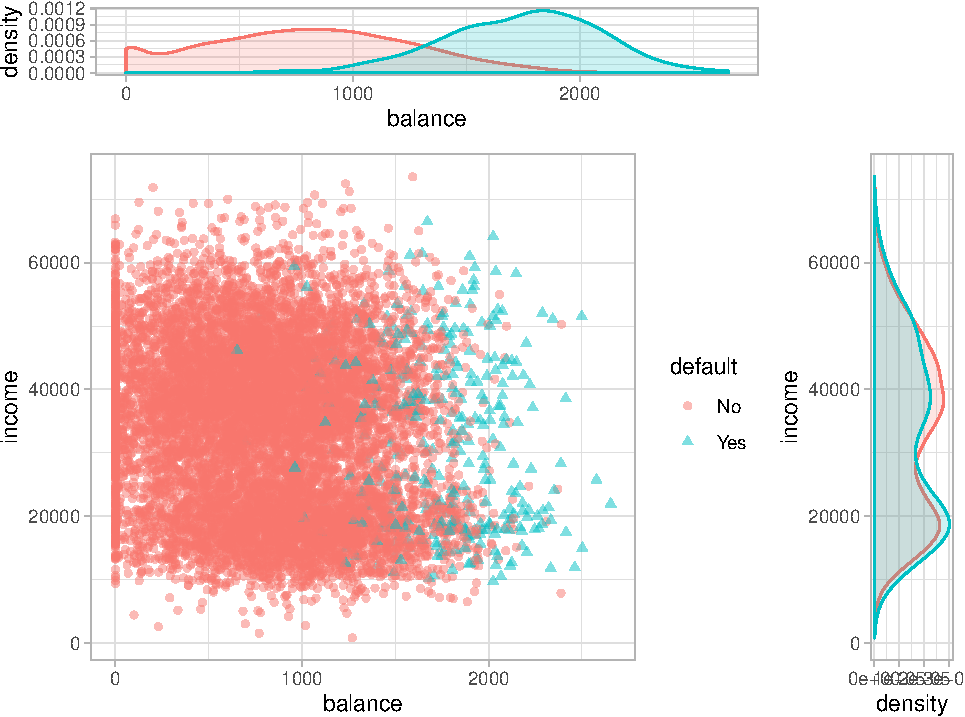
\includegraphics[width=0.8\linewidth]{_main_files/figure-latex/unnamed-chunk-38-1} \end{center}

\hypertarget{LDA}{%
\section{Análisis Discriminante Lineal}\label{LDA}}

\begin{Shaded}
\begin{Highlighting}[]
\NormalTok{df <-}\StringTok{ }\NormalTok{Default[, }\KeywordTok{c}\NormalTok{(}\StringTok{"income"}\NormalTok{, }\StringTok{"balance"}\NormalTok{, }\StringTok{"default"}\NormalTok{)]}
\KeywordTok{set.seed}\NormalTok{(}\DecValTok{123}\NormalTok{)}
\NormalTok{train.ID <-}\StringTok{ }\KeywordTok{createDataPartition}\NormalTok{(df}\OperatorTok{$}\NormalTok{default, }\DataTypeTok{p =} \FloatTok{0.8}\NormalTok{, }\DataTypeTok{list =} \OtherTok{FALSE}\NormalTok{)}

\NormalTok{train_df <-}\StringTok{ }\NormalTok{df[train.ID, ]}
\NormalTok{test_df <-}\StringTok{ }\NormalTok{df[}\OperatorTok{-}\NormalTok{train.ID, ]}

\CommentTok{# definimos como control una validación cruzada con 10 hojas, sin repeticiones}
\NormalTok{fit_control <-}\StringTok{ }\KeywordTok{trainControl}\NormalTok{(}\DataTypeTok{method=}\StringTok{'cv'}\NormalTok{, }\DataTypeTok{number =} \DecValTok{10}\NormalTok{)}

\KeywordTok{set.seed}\NormalTok{(}\DecValTok{123}\NormalTok{)}
\NormalTok{model_lda_def <-}\StringTok{ }\KeywordTok{train}\NormalTok{(default }\OperatorTok{~}\NormalTok{.,}
                       \DataTypeTok{data =}\NormalTok{ train_df,}
                       \DataTypeTok{method =} \StringTok{"lda"}\NormalTok{,}
                       \DataTypeTok{trControl =}\NormalTok{ fit_control)}
\NormalTok{model_lda_def}
\end{Highlighting}
\end{Shaded}

\begin{verbatim}
## Linear Discriminant Analysis 
## 
## 8001 samples
##    2 predictor
##    2 classes: 'No', 'Yes' 
## 
## No pre-processing
## Resampling: Cross-Validated (10 fold) 
## Summary of sample sizes: 7200, 7200, 7201, 7202, 7201, 7202, ... 
## Resampling results:
## 
##   Accuracy  Kappa    
##   0.973379  0.3710518
\end{verbatim}

\begin{Shaded}
\begin{Highlighting}[]
\NormalTok{model_lda_def}\OperatorTok{$}\NormalTok{finalModel}
\end{Highlighting}
\end{Shaded}

\begin{verbatim}
## Call:
## lda(x, grouping = y)
## 
## Prior probabilities of groups:
##         No        Yes 
## 0.96662917 0.03337083 
## 
## Group means:
##       income   balance
## No  33513.73  805.9109
## Yes 32450.16 1753.3628
## 
## Coefficients of linear discriminants:
##                  LD1
## income  9.334558e-06
## balance 2.233976e-03
\end{verbatim}

La precisión durante el entrenamiento es de un \(\approx 97\%\). También vemos que las probabilidades a priori \(\pi_i, i = 1,2\) de pertenecer a cada clase son aproximadamente \(97\%\) y \(3\%\) respectivamente, lo cual corresponde a la razón de fallo que se comenta al inicio. El resultado \texttt{Coefficients\ of\ linear\ discriminants} indica las constantes que se multiplican a cada elemento de la muestra \((\text{income}_i, \text{balance}_i)\), \(i = 1, \ldots, n_{\text{train}}\), para obtener su correspondiente valor de la \emph{función discriminante lineal}:
\[ \delta_k(x) = x^T \Sigma^{-1} \mu_k  - \dfrac{1}{2} \mu_k^T \Sigma^{-1} \mu_k+ log(\pi_k) \]
Todo indica que la variable \texttt{balance} tiene un mayor peso en la discriminación. Como alternativa, podemos comprobarlo usando \texttt{varImp}:

\begin{Shaded}
\begin{Highlighting}[]
\KeywordTok{varImp}\NormalTok{(model_lda_def)}
\end{Highlighting}
\end{Shaded}

\begin{verbatim}
## ROC curve variable importance
## 
##         Importance
## balance        100
## income           0
\end{verbatim}

Veamos ahora qué tal es el ajuste en los datos test.

\begin{Shaded}
\begin{Highlighting}[]
\CommentTok{# hagamos las predicciones del conjunto de prueba}
\NormalTok{prediction_lda_def <-}\StringTok{ }\KeywordTok{predict}\NormalTok{(model_lda_def, }\DataTypeTok{newdata =}\NormalTok{ test_df)}
\KeywordTok{confusionMatrix}\NormalTok{(prediction_lda_def, }\DataTypeTok{reference =}\NormalTok{ test_df}\OperatorTok{$}\NormalTok{default)}
\end{Highlighting}
\end{Shaded}

\begin{verbatim}
## Confusion Matrix and Statistics
## 
##           Reference
## Prediction   No  Yes
##        No  1927   54
##        Yes    6   12
##                                          
##                Accuracy : 0.97           
##                  95% CI : (0.9615, 0.977)
##     No Information Rate : 0.967          
##     P-Value [Acc > NIR] : 0.2488         
##                                          
##                   Kappa : 0.2755         
##                                          
##  Mcnemar's Test P-Value : 1.298e-09      
##                                          
##             Sensitivity : 0.9969         
##             Specificity : 0.1818         
##          Pos Pred Value : 0.9727         
##          Neg Pred Value : 0.6667         
##              Prevalence : 0.9670         
##          Detection Rate : 0.9640         
##    Detection Prevalence : 0.9910         
##       Balanced Accuracy : 0.5894         
##                                          
##        'Positive' Class : No             
## 
\end{verbatim}

\begin{Shaded}
\begin{Highlighting}[]
\CommentTok{# extraemos el Accuracy o Precisión}
\KeywordTok{confusionMatrix}\NormalTok{(prediction_lda_def, }\DataTypeTok{reference =}\NormalTok{ test_df}\OperatorTok{$}\NormalTok{default)}\OperatorTok{$}\NormalTok{overall[}\DecValTok{1}\NormalTok{]}
\end{Highlighting}
\end{Shaded}

\begin{verbatim}
## Accuracy 
## 0.969985
\end{verbatim}

\begin{Shaded}
\begin{Highlighting}[]
\CommentTok{# la tasa de error}
\NormalTok{tasa.error.lda <-}\StringTok{ }\DecValTok{1}\OperatorTok{-}\KeywordTok{confusionMatrix}\NormalTok{(prediction_lda_def, }\DataTypeTok{reference =}\NormalTok{ test_df}\OperatorTok{$}\NormalTok{default)}\OperatorTok{$}\NormalTok{overall[}\DecValTok{1}\NormalTok{]}
\KeywordTok{names}\NormalTok{(tasa.error.lda) <-}\StringTok{ "Error LDA"}
\NormalTok{tasa.error.lda}
\end{Highlighting}
\end{Shaded}

\begin{verbatim}
##  Error LDA 
## 0.03001501
\end{verbatim}

Como estamos en un problema de clasificación en dos dimensiones (\(p = 2\)), es posible representar la frontera de decisión del algoritmo, usando la función \texttt{decision\_bound}. Debemos modificar los campos para que coincidan con las variables de \texttt{Default}:

\begin{Shaded}
\begin{Highlighting}[]
\NormalTok{decision_bound =}\StringTok{ }\ControlFlowTok{function}\NormalTok{(train_df_in, test_df_in, model_in)\{}
  \CommentTok{# plot decision boundary  for df <- Default[, c("income", "balance", "default")]}

  \KeywordTok{require}\NormalTok{(MASS)}
  \KeywordTok{require}\NormalTok{(caret)}
  \KeywordTok{require}\NormalTok{(ggplot2)}
  \KeywordTok{require}\NormalTok{(gridExtra)}

  \CommentTok{# Paso 1: crear un grid de valores desde min a max de ambos predictores}
\NormalTok{  pl =}\StringTok{ }\KeywordTok{seq}\NormalTok{(}\KeywordTok{min}\NormalTok{(train_df_in}\OperatorTok{$}\NormalTok{balance), }\KeywordTok{max}\NormalTok{(train_df_in}\OperatorTok{$}\NormalTok{balance), }\DataTypeTok{length.out =} \DecValTok{80}\NormalTok{)}
\NormalTok{  pw =}\StringTok{ }\KeywordTok{seq}\NormalTok{(}\KeywordTok{min}\NormalTok{(train_df_in}\OperatorTok{$}\NormalTok{income), }\KeywordTok{max}\NormalTok{(train_df_in}\OperatorTok{$}\NormalTok{income), }\DataTypeTok{length.out =} \DecValTok{80}\NormalTok{)}

\NormalTok{  lgrid <-}\StringTok{ }\KeywordTok{expand.grid}\NormalTok{(}\DataTypeTok{balance=}\NormalTok{pl, }\DataTypeTok{income=}\NormalTok{pw)}

  \CommentTok{# Paso 2: obtener las predicciones tanto para el grid como para el test}
\NormalTok{  modelPredGrid <-}\StringTok{ }\KeywordTok{predict}\NormalTok{(model_in, }\DataTypeTok{newdata=}\NormalTok{lgrid)}
\NormalTok{  train_df_in}\OperatorTok{$}\NormalTok{Pred.Class <-}\StringTok{ }\KeywordTok{predict}\NormalTok{(model_in, }\DataTypeTok{newdata =}\NormalTok{ train_df_in)}
\NormalTok{  test_df_in}\OperatorTok{$}\NormalTok{Pred.Class <-}\StringTok{ }\KeywordTok{predict}\NormalTok{(model_in, }\DataTypeTok{newdata =}\NormalTok{ test_df_in)}

  \CommentTok{# Paso 3: ggplot con la funcion contour}
\NormalTok{  gg1 <-}\StringTok{ }\KeywordTok{ggplot}\NormalTok{(}\DataTypeTok{data=}\NormalTok{lgrid) }\OperatorTok{+}
\StringTok{    }\KeywordTok{stat_contour}\NormalTok{(}\KeywordTok{aes}\NormalTok{(}\DataTypeTok{x=}\NormalTok{balance, }\DataTypeTok{y=}\NormalTok{income, }\DataTypeTok{z=}\KeywordTok{as.numeric}\NormalTok{(modelPredGrid)), }\DataTypeTok{bins=}\DecValTok{2}\NormalTok{) }\OperatorTok{+}
\StringTok{    }\KeywordTok{geom_point}\NormalTok{(}\KeywordTok{aes}\NormalTok{(}\DataTypeTok{x=}\NormalTok{balance, }\DataTypeTok{y=}\NormalTok{income, }\DataTypeTok{colour=}\NormalTok{modelPredGrid), }\DataTypeTok{alpha=}\FloatTok{0.1}\NormalTok{) }\OperatorTok{+}
\StringTok{    }\KeywordTok{labs}\NormalTok{(}\DataTypeTok{colour =} \StringTok{"Clases"}\NormalTok{) }\OperatorTok{+}\StringTok{ }\KeywordTok{ggtitle}\NormalTok{(}\StringTok{"Train"}\NormalTok{) }\OperatorTok{+}
\StringTok{    }\KeywordTok{geom_point}\NormalTok{(}\DataTypeTok{data=}\NormalTok{train_df_in,}
               \KeywordTok{aes}\NormalTok{(}\DataTypeTok{x=}\NormalTok{balance, }\DataTypeTok{y=}\NormalTok{income,}
                   \DataTypeTok{colour=}\NormalTok{default), }\DataTypeTok{size=}\DecValTok{5}\NormalTok{, }\DataTypeTok{shape=}\DecValTok{1}\NormalTok{) }\OperatorTok{+}
\StringTok{    }\KeywordTok{theme_light}\NormalTok{()}

\NormalTok{  gg2 <-}\StringTok{ }\KeywordTok{ggplot}\NormalTok{(}\DataTypeTok{data=}\NormalTok{lgrid) }\OperatorTok{+}
\StringTok{    }\KeywordTok{stat_contour}\NormalTok{(}\KeywordTok{aes}\NormalTok{(}\DataTypeTok{x=}\NormalTok{balance, }\DataTypeTok{y=}\NormalTok{income, }\DataTypeTok{z=}\KeywordTok{as.numeric}\NormalTok{(modelPredGrid)), }\DataTypeTok{bins=}\DecValTok{2}\NormalTok{) }\OperatorTok{+}
\StringTok{    }\KeywordTok{geom_point}\NormalTok{(}\KeywordTok{aes}\NormalTok{(}\DataTypeTok{x=}\NormalTok{balance, }\DataTypeTok{y=}\NormalTok{income, }\DataTypeTok{colour=}\NormalTok{modelPredGrid), }\DataTypeTok{alpha=}\FloatTok{0.1}\NormalTok{) }\OperatorTok{+}
\StringTok{    }\KeywordTok{labs}\NormalTok{(}\DataTypeTok{colour =} \StringTok{"Clases"}\NormalTok{) }\OperatorTok{+}\StringTok{ }\KeywordTok{ggtitle}\NormalTok{(}\StringTok{"Test"}\NormalTok{) }\OperatorTok{+}
\StringTok{    }\KeywordTok{geom_point}\NormalTok{(}\DataTypeTok{data=}\NormalTok{test_df_in,}
               \KeywordTok{aes}\NormalTok{(}\DataTypeTok{x=}\NormalTok{balance, }\DataTypeTok{y=}\NormalTok{income,}
                   \DataTypeTok{colour=}\NormalTok{default), }\DataTypeTok{size=}\DecValTok{5}\NormalTok{, }\DataTypeTok{shape=}\DecValTok{1}\NormalTok{) }\OperatorTok{+}
\StringTok{    }\KeywordTok{theme_light}\NormalTok{()}
  \KeywordTok{grid.arrange}\NormalTok{(gg1, gg2, }\DataTypeTok{ncol=}\DecValTok{1}\NormalTok{, }\DataTypeTok{nrow=}\DecValTok{2}\NormalTok{)}
\NormalTok{\}}
\end{Highlighting}
\end{Shaded}

\begin{Shaded}
\begin{Highlighting}[]
\KeywordTok{decision_bound}\NormalTok{(train_df, test_df, model_lda_def)}
\end{Highlighting}
\end{Shaded}

\begin{center}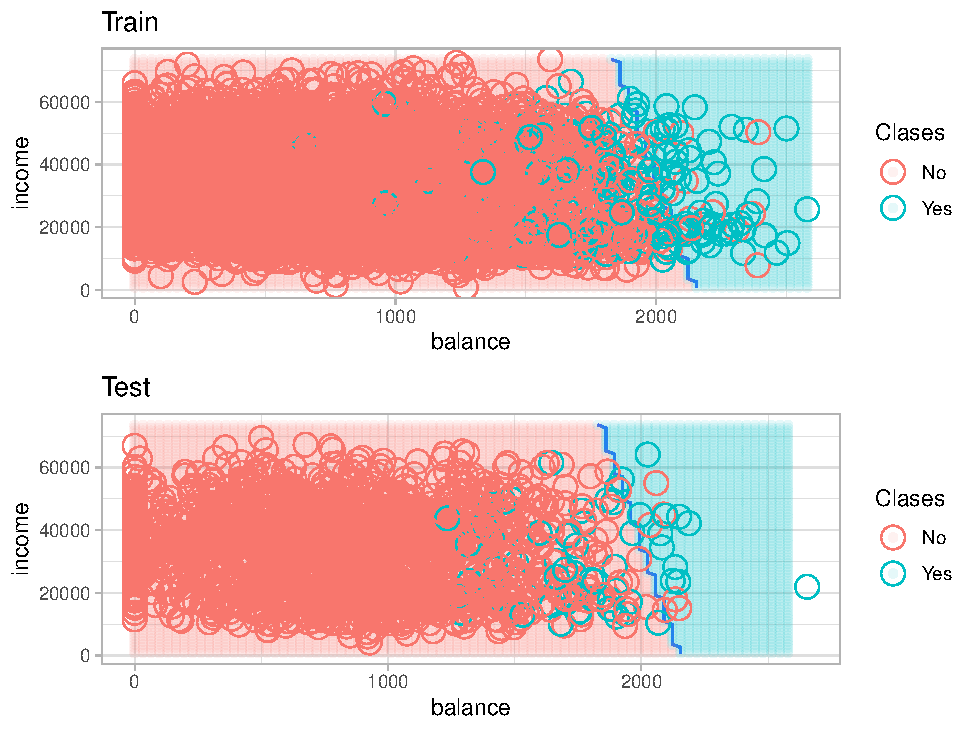
\includegraphics[width=0.8\linewidth]{_main_files/figure-latex/unnamed-chunk-43-1} \end{center}

\hypertarget{QDA}{%
\section{Análisis Discriminante Cuadrático}\label{QDA}}

El ajuste para el modelo QDA lo hacemos con el mismo control y la misma partición de la muestra.

\begin{Shaded}
\begin{Highlighting}[]
\KeywordTok{set.seed}\NormalTok{(}\DecValTok{123}\NormalTok{)}
\NormalTok{model_qda_def <-}\StringTok{ }\KeywordTok{train}\NormalTok{(default }\OperatorTok{~}\NormalTok{.,}
                       \DataTypeTok{data =}\NormalTok{ train_df,}
                       \DataTypeTok{method =} \StringTok{"qda"}\NormalTok{,}
                       \DataTypeTok{trControl =}\NormalTok{ fit_control)}
\NormalTok{model_qda_def}
\end{Highlighting}
\end{Shaded}

\begin{verbatim}
## Quadratic Discriminant Analysis 
## 
## 8001 samples
##    2 predictor
##    2 classes: 'No', 'Yes' 
## 
## No pre-processing
## Resampling: Cross-Validated (10 fold) 
## Summary of sample sizes: 7200, 7200, 7201, 7202, 7201, 7202, ... 
## Resampling results:
## 
##   Accuracy   Kappa    
##   0.9730043  0.3787741
\end{verbatim}

\begin{Shaded}
\begin{Highlighting}[]
\NormalTok{model_qda_def}\OperatorTok{$}\NormalTok{finalModel}
\end{Highlighting}
\end{Shaded}

\begin{verbatim}
## Call:
## qda(x, grouping = y)
## 
## Prior probabilities of groups:
##         No        Yes 
## 0.96662917 0.03337083 
## 
## Group means:
##       income   balance
## No  33513.73  805.9109
## Yes 32450.16 1753.3628
\end{verbatim}

Los resultados al entrenar son similares al caso LDA. Veamos las predicciones para la muestra test.

\begin{Shaded}
\begin{Highlighting}[]
\CommentTok{# hagamos las predicciones del conjunto de prueba}
\NormalTok{prediction_qda_def <-}\StringTok{ }\KeywordTok{predict}\NormalTok{(model_qda_def, }\DataTypeTok{newdata =}\NormalTok{ test_df)}
\KeywordTok{confusionMatrix}\NormalTok{(prediction_qda_def, }\DataTypeTok{reference =}\NormalTok{ test_df}\OperatorTok{$}\NormalTok{default)}
\end{Highlighting}
\end{Shaded}

\begin{verbatim}
## Confusion Matrix and Statistics
## 
##           Reference
## Prediction   No  Yes
##        No  1924   51
##        Yes    9   15
##                                          
##                Accuracy : 0.97           
##                  95% CI : (0.9615, 0.977)
##     No Information Rate : 0.967          
##     P-Value [Acc > NIR] : 0.2488         
##                                          
##                   Kappa : 0.3214         
##                                          
##  Mcnemar's Test P-Value : 1.203e-07      
##                                          
##             Sensitivity : 0.9953         
##             Specificity : 0.2273         
##          Pos Pred Value : 0.9742         
##          Neg Pred Value : 0.6250         
##              Prevalence : 0.9670         
##          Detection Rate : 0.9625         
##    Detection Prevalence : 0.9880         
##       Balanced Accuracy : 0.6113         
##                                          
##        'Positive' Class : No             
## 
\end{verbatim}

\begin{Shaded}
\begin{Highlighting}[]
\CommentTok{# extraemos el Accuracy o Precisión}
\KeywordTok{confusionMatrix}\NormalTok{(prediction_qda_def, }\DataTypeTok{reference =}\NormalTok{ test_df}\OperatorTok{$}\NormalTok{default)}\OperatorTok{$}\NormalTok{overall[}\DecValTok{1}\NormalTok{]}
\end{Highlighting}
\end{Shaded}

\begin{verbatim}
## Accuracy 
## 0.969985
\end{verbatim}

\begin{Shaded}
\begin{Highlighting}[]
\CommentTok{# la tasa de error}
\NormalTok{tasa.error.qda <-}\StringTok{ }\DecValTok{1}\OperatorTok{-}\KeywordTok{confusionMatrix}\NormalTok{(prediction_qda_def, }\DataTypeTok{reference =}\NormalTok{ test_df}\OperatorTok{$}\NormalTok{default)}\OperatorTok{$}\NormalTok{overall[}\DecValTok{1}\NormalTok{]}
\KeywordTok{names}\NormalTok{(tasa.error.qda) <-}\StringTok{ "Error QDA"}
\NormalTok{tasa.error.qda}
\end{Highlighting}
\end{Shaded}

\begin{verbatim}
##  Error QDA 
## 0.03001501
\end{verbatim}

Tampoco se logran mejorar los resultados. Finalmente, representamos la frontera de decisión del algoritmo.

\begin{Shaded}
\begin{Highlighting}[]
\KeywordTok{decision_bound}\NormalTok{(train_df, test_df, model_qda_def)}
\end{Highlighting}
\end{Shaded}

\begin{center}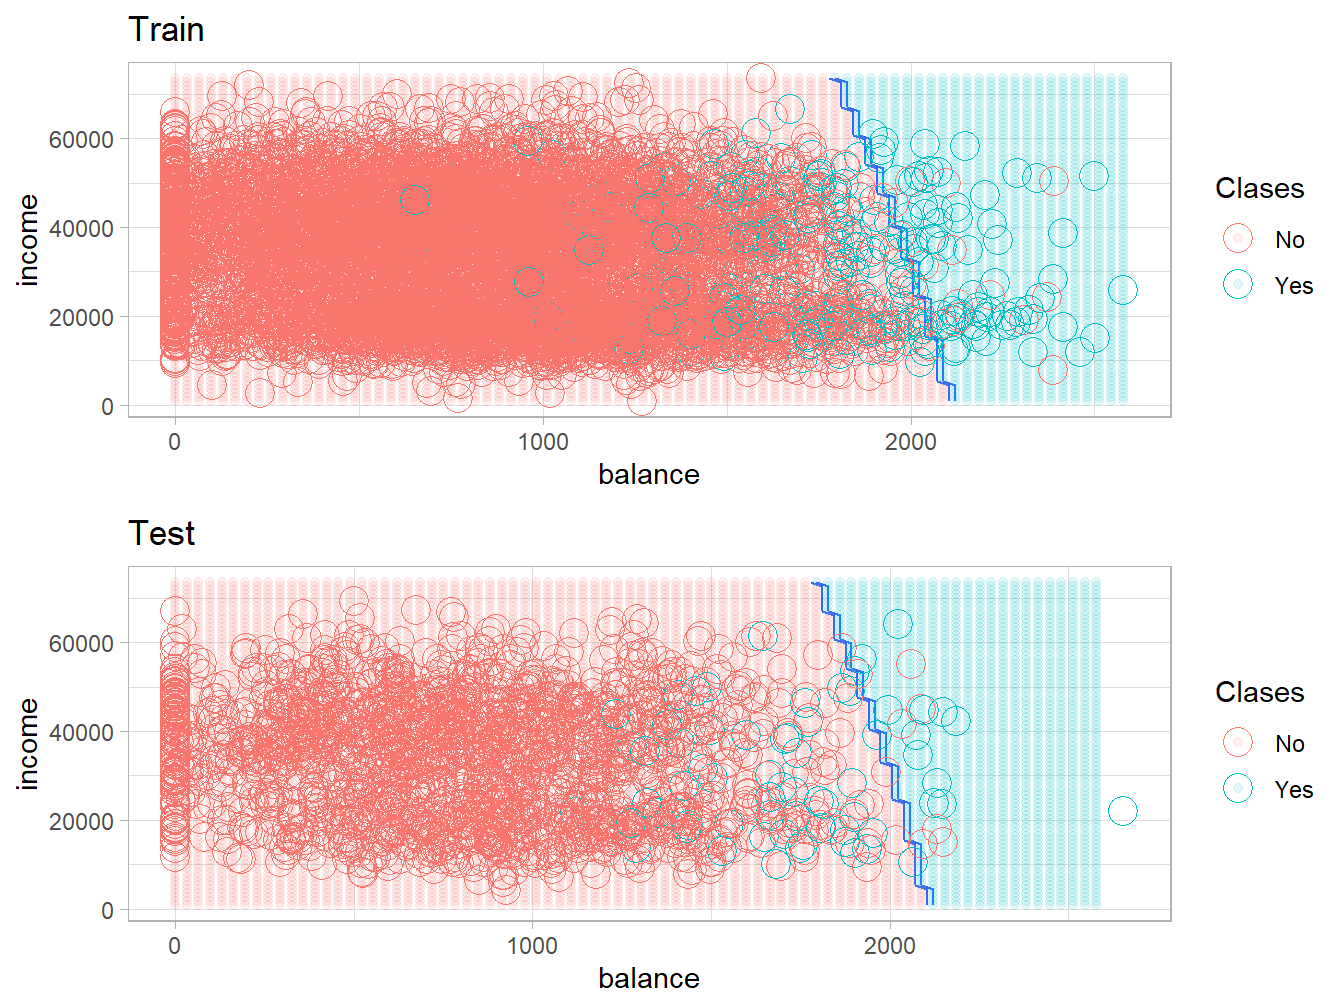
\includegraphics[width=0.8\linewidth]{_main_files/figure-latex/unnamed-chunk-46-1} \end{center}

¡Ahora observamos que las regiones están separadas por curvas, en lugar de la recta del LDA!

\hypertarget{RDA}{%
\section{Análisis Discriminante Regularizado}\label{RDA}}

\textbf{Opción 1}: el paquete \texttt{caret} crea el grid para \((\lambda, \gamma)\):

\begin{Shaded}
\begin{Highlighting}[]
\KeywordTok{set.seed}\NormalTok{(}\DecValTok{123}\NormalTok{)}
\NormalTok{model_rda_def <-}\StringTok{ }\KeywordTok{train}\NormalTok{(default }\OperatorTok{~}\NormalTok{.,}
                       \DataTypeTok{data =}\NormalTok{ train_df,}
                       \DataTypeTok{method =} \StringTok{"rda"}\NormalTok{,}
                       \DataTypeTok{tuneLength =} \DecValTok{2}\NormalTok{,}
                       \DataTypeTok{trControl =}\NormalTok{ fit_control)}

\NormalTok{model_rda_def}
\end{Highlighting}
\end{Shaded}

\begin{verbatim}
## Regularized Discriminant Analysis 
## 
## 8001 samples
##    2 predictor
##    2 classes: 'No', 'Yes' 
## 
## No pre-processing
## Resampling: Cross-Validated (10 fold) 
## Summary of sample sizes: 7200, 7200, 7201, 7202, 7201, 7202, ... 
## Resampling results across tuning parameters:
## 
##   gamma  lambda  Accuracy   Kappa    
##   0      0       0.9730043  0.3787741
##   0      1       0.9733790  0.3710518
##   1      0       0.9666297  0.0000000
##   1      1       0.9666297  0.0000000
## 
## Accuracy was used to select the optimal model using the largest value.
## The final values used for the model were gamma = 0 and lambda = 1.
\end{verbatim}

\begin{Shaded}
\begin{Highlighting}[]
\NormalTok{model_rda_def}\OperatorTok{$}\NormalTok{finalModel}
\end{Highlighting}
\end{Shaded}

\begin{verbatim}
## Call: 
## rda.default(x = x, grouping = y, gamma = param$gamma, lambda = param$lambda)
## 
## Regularization parameters: 
##  gamma lambda 
##      0      1 
## 
## Prior probabilities of groups: 
##         No        Yes 
## 0.96662917 0.03337083 
## 
## Misclassification rate: 
##        apparent: 2.662 %
\end{verbatim}

\begin{Shaded}
\begin{Highlighting}[]
\CommentTok{# en este caso el ggplot nos da información sobre los }
\CommentTok{# hiperparametros y su correspondiente Accuracy}
\KeywordTok{ggplot}\NormalTok{(model_rda_def) }\OperatorTok{+}\StringTok{ }\KeywordTok{theme_light}\NormalTok{()}
\end{Highlighting}
\end{Shaded}

\begin{center}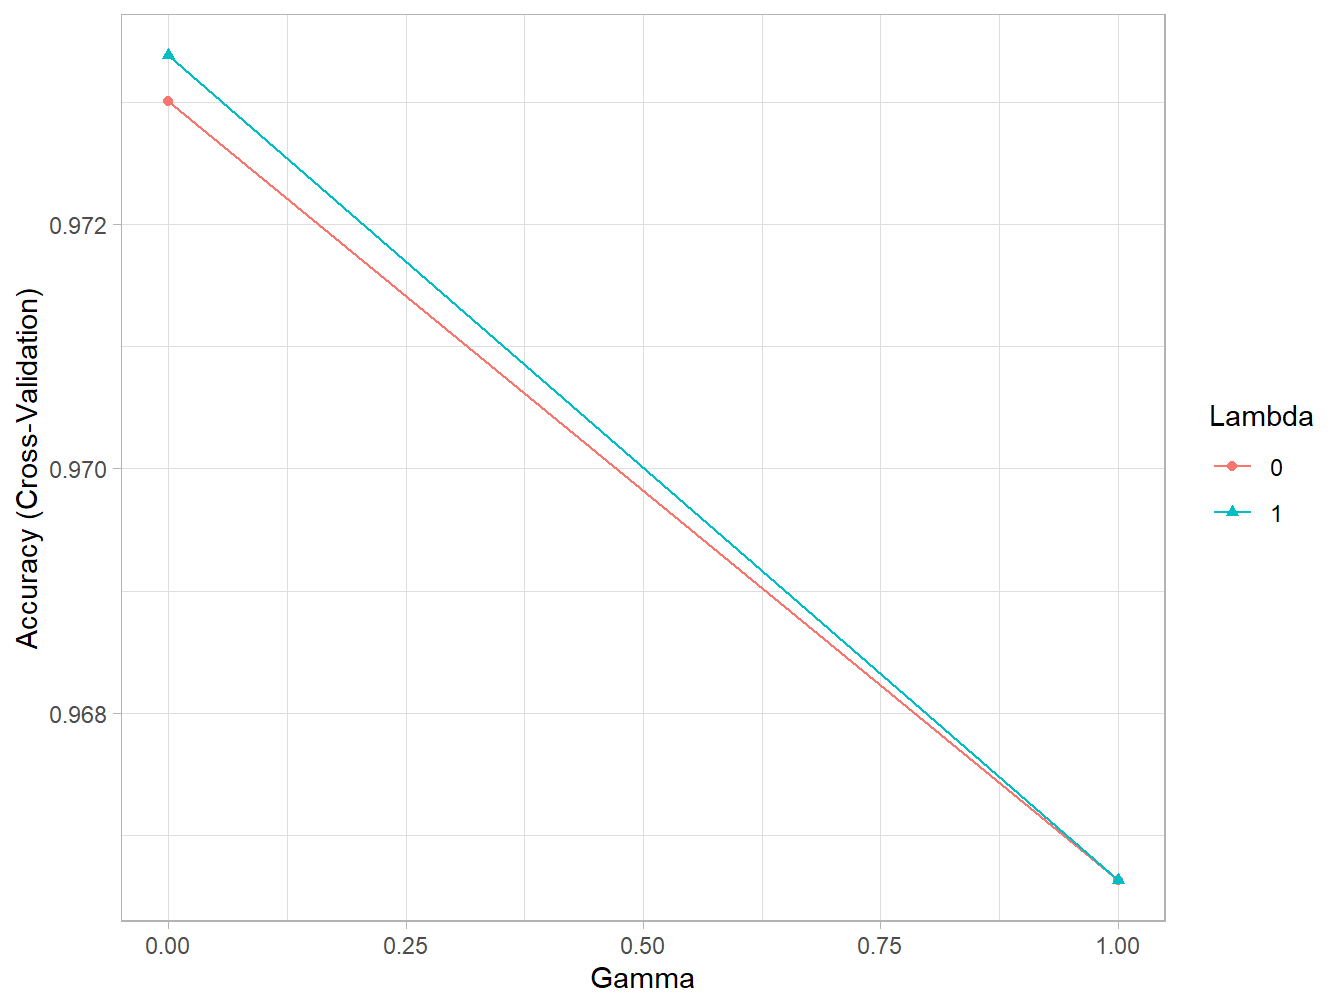
\includegraphics[width=0.8\linewidth]{_main_files/figure-latex/unnamed-chunk-48-1} \end{center}

\textbf{Opción 2}: podemos proporcionar un grid predefinido de valores \((\lambda, \gamma)\) en un \texttt{data.frame} que le pasamos a \texttt{tuneGrid}:

\begin{Shaded}
\begin{Highlighting}[]
\CommentTok{# el grid se puede definir tambien "a mano"}
\NormalTok{mi.grid <-}\StringTok{ }\KeywordTok{data.frame}\NormalTok{(}\DataTypeTok{lambda =} \KeywordTok{c}\NormalTok{(}\DecValTok{0}\NormalTok{, }\FloatTok{0.3}\NormalTok{, }\FloatTok{0.6}\NormalTok{, }\DecValTok{1}\NormalTok{) , }
                       \DataTypeTok{gamma =} \KeywordTok{c}\NormalTok{(}\DecValTok{0}\NormalTok{, }\DecValTok{0}\NormalTok{, }\DecValTok{0}\NormalTok{, }\DecValTok{0}\NormalTok{))}
\KeywordTok{set.seed}\NormalTok{(}\DecValTok{123}\NormalTok{)}
\NormalTok{model_rda_def <-}\StringTok{ }\KeywordTok{train}\NormalTok{(default }\OperatorTok{~}\NormalTok{.,}
                       \DataTypeTok{data =}\NormalTok{ train_df,}
                       \DataTypeTok{method =} \StringTok{"rda"}\NormalTok{,}
                       \DataTypeTok{tuneGrid =}\NormalTok{ mi.grid,}
                       \DataTypeTok{trControl =}\NormalTok{ fit_control)}
\NormalTok{model_rda_def}
\end{Highlighting}
\end{Shaded}

\begin{verbatim}
## Regularized Discriminant Analysis 
## 
## 8001 samples
##    2 predictor
##    2 classes: 'No', 'Yes' 
## 
## No pre-processing
## Resampling: Cross-Validated (10 fold) 
## Summary of sample sizes: 7200, 7200, 7201, 7202, 7201, 7202, ... 
## Resampling results across tuning parameters:
## 
##   lambda  Accuracy   Kappa    
##   0.0     0.9730043  0.3787741
##   0.3     0.9733790  0.3791078
##   0.6     0.9735039  0.3764691
##   1.0     0.9733790  0.3710518
## 
## Tuning parameter 'gamma' was held constant at a value of 0
## Accuracy was used to select the optimal model using the largest value.
## The final values used for the model were gamma = 0 and lambda = 0.6.
\end{verbatim}

\begin{Shaded}
\begin{Highlighting}[]
\NormalTok{model_rda_def}\OperatorTok{$}\NormalTok{finalModel}
\end{Highlighting}
\end{Shaded}

\begin{verbatim}
## Call: 
## rda.default(x = x, grouping = y, gamma = param$gamma, lambda = param$lambda)
## 
## Regularization parameters: 
##  gamma lambda 
##    0.0    0.6 
## 
## Prior probabilities of groups: 
##         No        Yes 
## 0.96662917 0.03337083 
## 
## Misclassification rate: 
##        apparent: 2.675 %
\end{verbatim}

\begin{Shaded}
\begin{Highlighting}[]
\CommentTok{# en este caso el ggplot nos da información sobre los }
\CommentTok{# hiperparametros y su correspondiente Accuracy}
\KeywordTok{ggplot}\NormalTok{(model_rda_def) }\OperatorTok{+}\StringTok{ }\KeywordTok{theme_light}\NormalTok{()}
\end{Highlighting}
\end{Shaded}

\begin{center}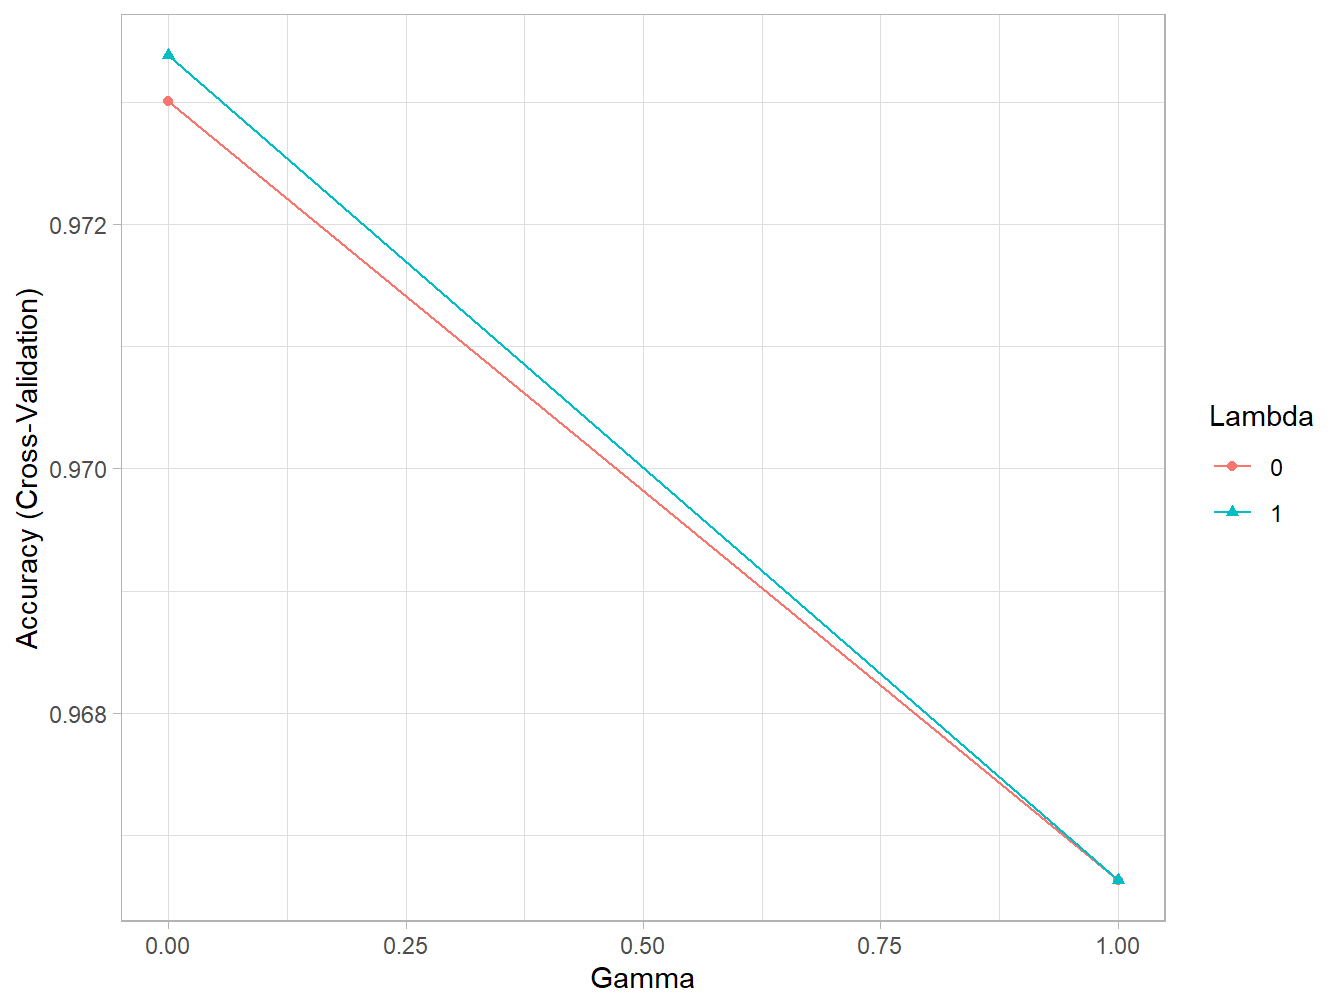
\includegraphics[width=0.8\linewidth]{_main_files/figure-latex/unnamed-chunk-50-1} \end{center}

Los resultados indican que los hiperparámetros óptimos en este caso corresponden a \((\lambda, \gamma) = (0,0)\). ¡Este es el caso del algoritmo LDA! Esto que hemos hecho es comparar diferentes modelos (porque han sido ajustados con diferentes hiperparámetros) resultantes del mismo algoritmo. Veamos las predicciones para la muestra test, la tasa de error correspondiente y la frontera de decisión.

\begin{Shaded}
\begin{Highlighting}[]
\CommentTok{# hagamos las predicciones del conjunto de prueba}
\NormalTok{prediction_rda_def <-}\StringTok{ }\KeywordTok{predict}\NormalTok{(model_rda_def, }\DataTypeTok{newdata =}\NormalTok{ test_df)}
\KeywordTok{confusionMatrix}\NormalTok{(prediction_rda_def, }\DataTypeTok{reference =}\NormalTok{ test_df}\OperatorTok{$}\NormalTok{default)}
\end{Highlighting}
\end{Shaded}

\begin{verbatim}
## Confusion Matrix and Statistics
## 
##           Reference
## Prediction   No  Yes
##        No  1926   52
##        Yes    7   14
##                                           
##                Accuracy : 0.9705          
##                  95% CI : (0.9621, 0.9775)
##     No Information Rate : 0.967           
##     P-Value [Acc > NIR] : 0.2098          
##                                           
##                   Kappa : 0.3109          
##                                           
##  Mcnemar's Test P-Value : 1.014e-08       
##                                           
##             Sensitivity : 0.9964          
##             Specificity : 0.2121          
##          Pos Pred Value : 0.9737          
##          Neg Pred Value : 0.6667          
##              Prevalence : 0.9670          
##          Detection Rate : 0.9635          
##    Detection Prevalence : 0.9895          
##       Balanced Accuracy : 0.6042          
##                                           
##        'Positive' Class : No              
## 
\end{verbatim}

\begin{Shaded}
\begin{Highlighting}[]
\CommentTok{# extraemos el Accuracy o Precisión}
\KeywordTok{confusionMatrix}\NormalTok{(prediction_rda_def, }\DataTypeTok{reference =}\NormalTok{ test_df}\OperatorTok{$}\NormalTok{default)}\OperatorTok{$}\NormalTok{overall[}\DecValTok{1}\NormalTok{]}
\end{Highlighting}
\end{Shaded}

\begin{verbatim}
##  Accuracy 
## 0.9704852
\end{verbatim}

\begin{Shaded}
\begin{Highlighting}[]
\CommentTok{# la tasa de error}
\NormalTok{tasa.error.rda <-}\StringTok{ }\DecValTok{1}\OperatorTok{-}\KeywordTok{confusionMatrix}\NormalTok{(prediction_rda_def, }\DataTypeTok{reference =}\NormalTok{ test_df}\OperatorTok{$}\NormalTok{default)}\OperatorTok{$}\NormalTok{overall[}\DecValTok{1}\NormalTok{]}
\KeywordTok{names}\NormalTok{(tasa.error.rda) <-}\StringTok{ "Error RDA"}
\NormalTok{tasa.error.rda}
\end{Highlighting}
\end{Shaded}

\begin{verbatim}
##  Error RDA 
## 0.02951476
\end{verbatim}

\begin{Shaded}
\begin{Highlighting}[]
\KeywordTok{decision_bound}\NormalTok{(train_df, test_df, model_rda_def)}
\end{Highlighting}
\end{Shaded}

\begin{center}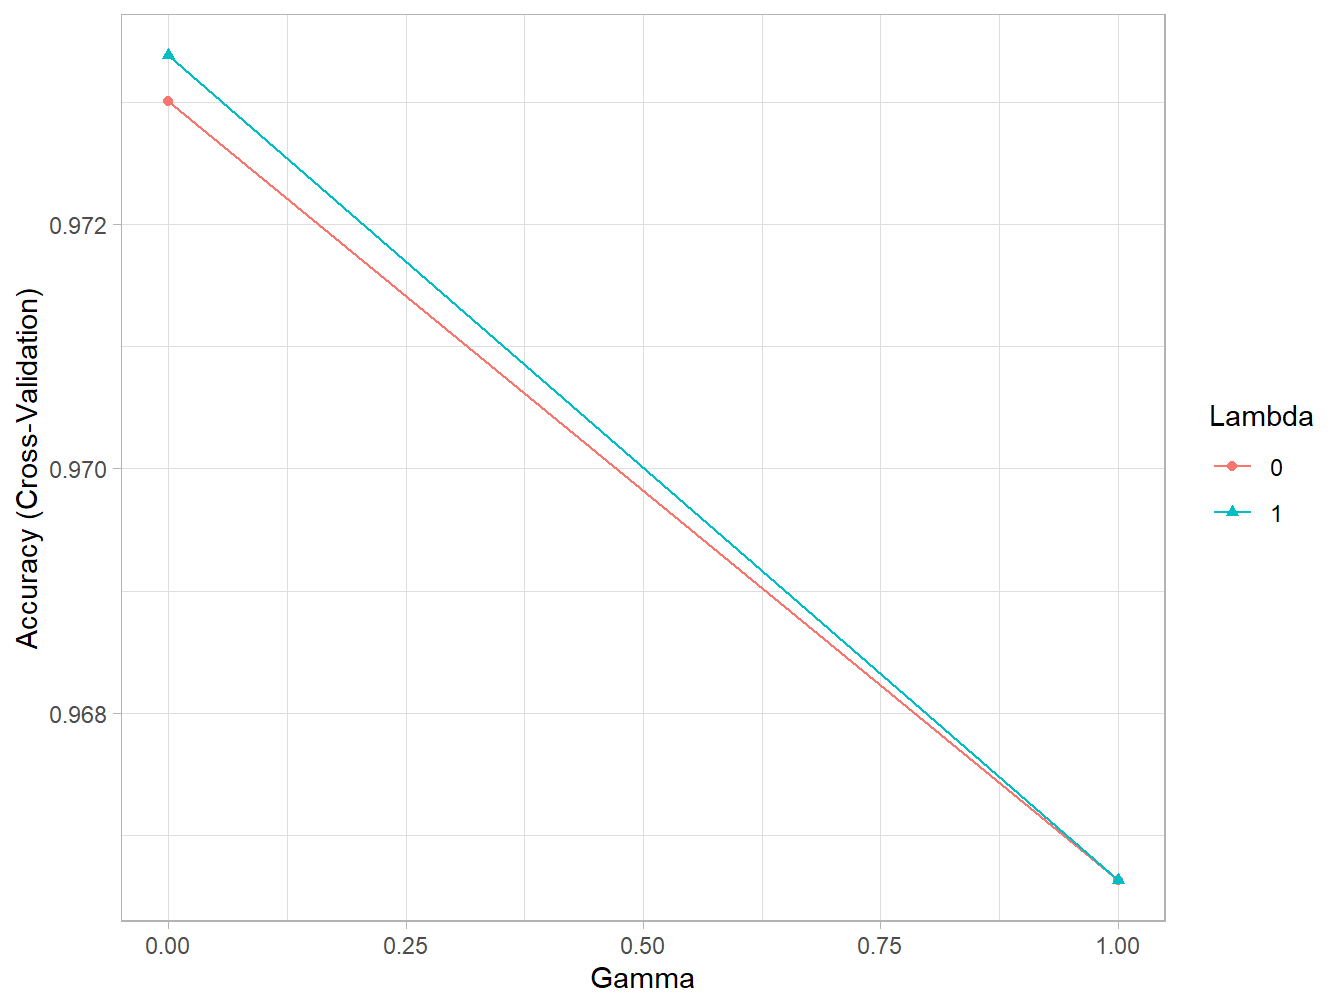
\includegraphics[width=0.8\linewidth]{_main_files/figure-latex/unnamed-chunk-52-1} \end{center}

\hypertarget{compara}{%
\chapter{Comparación entre Modelos}\label{compara}}

Hasta ahora hemos visto cómo comparar el ajuste de un modelo para diferentes hiperparámetros, por ejemplo, en el caso RDA se escoge el modelo con mayor \texttt{Accuracy} para diferentes combinaciones de \((\lambda, \gamma)\); o la selección del \(K\) óptimo en KNN. Este enfoque lo que hace es estudiar la distribución del \texttt{Accuracy} (o cualquier otra medida de precisión como el \texttt{Kappa}) para cada modelo independientemente (\emph{within-model}).

El enfoque que abordamos en esta sección es la comparación de las distribuciones de estas medidas de precisión, ahora entre los diferentes modelos (\emph{between-models}).

\hypertarget{comparando-seguxfan-accuracy}{%
\section{\texorpdfstring{Comparando según \texttt{Accuracy}}{Comparando según Accuracy}}\label{comparando-seguxfan-accuracy}}

Empezamos comparando los modelos ajustados en la Sección \ref{DA}. Vamos a usar los mismos datos de entrenamiento para cada modelo, y además ``plantaremos una semilla'' para que el remuestreo se haga en los mismos conjuntos.

\begin{Shaded}
\begin{Highlighting}[]
\KeywordTok{library}\NormalTok{(caret)}
\KeywordTok{library}\NormalTok{(ISLR)}

\NormalTok{df <-}\StringTok{ }\NormalTok{Default[, }\KeywordTok{c}\NormalTok{(}\StringTok{"income"}\NormalTok{, }\StringTok{"balance"}\NormalTok{, }\StringTok{"default"}\NormalTok{)]}
\KeywordTok{set.seed}\NormalTok{(}\DecValTok{123}\NormalTok{)}
\NormalTok{train.ID <-}\StringTok{ }\KeywordTok{createDataPartition}\NormalTok{(df}\OperatorTok{$}\NormalTok{default, }\DataTypeTok{p =} \FloatTok{0.8}\NormalTok{, }\DataTypeTok{list =} \OtherTok{FALSE}\NormalTok{)}

\NormalTok{train_df <-}\StringTok{ }\NormalTok{df[train.ID, ]}
\NormalTok{test_df <-}\StringTok{ }\NormalTok{df[}\OperatorTok{-}\NormalTok{train.ID, ]}

\CommentTok{# definimos como control una validación cruzada con 10 hojas y repeticiones}
\NormalTok{fit_control <-}\StringTok{ }\KeywordTok{trainControl}\NormalTok{(}\DataTypeTok{method=}\StringTok{'repeatedcv'}\NormalTok{, }\DataTypeTok{number =} \DecValTok{10}\NormalTok{, }\DataTypeTok{repeats =} \DecValTok{5}\NormalTok{)}
\end{Highlighting}
\end{Shaded}

\textbf{LDA}:

\begin{Shaded}
\begin{Highlighting}[]
\CommentTok{# LDA}
\KeywordTok{set.seed}\NormalTok{(}\DecValTok{321}\NormalTok{)}
\NormalTok{model_lda_def <-}\StringTok{ }\KeywordTok{train}\NormalTok{(default }\OperatorTok{~}\NormalTok{.,}
                       \DataTypeTok{data =}\NormalTok{ train_df,}
                       \DataTypeTok{method =} \StringTok{"lda"}\NormalTok{,}
                       \DataTypeTok{trControl =}\NormalTok{ fit_control)}
\end{Highlighting}
\end{Shaded}

\textbf{QDA}:

\begin{Shaded}
\begin{Highlighting}[]
\CommentTok{# QDA}
\KeywordTok{set.seed}\NormalTok{(}\DecValTok{321}\NormalTok{)}
\NormalTok{model_qda_def <-}\StringTok{ }\KeywordTok{train}\NormalTok{(default }\OperatorTok{~}\NormalTok{.,}
                       \DataTypeTok{data =}\NormalTok{ train_df,}
                       \DataTypeTok{method =} \StringTok{"qda"}\NormalTok{,}
                       \DataTypeTok{trControl =}\NormalTok{ fit_control)}
\end{Highlighting}
\end{Shaded}

\textbf{RDA}:

\begin{Shaded}
\begin{Highlighting}[]
\CommentTok{# RDA}

\NormalTok{mi.grid <-}\StringTok{ }\KeywordTok{data.frame}\NormalTok{(}\DataTypeTok{lambda =} \KeywordTok{c}\NormalTok{(}\DecValTok{0}\NormalTok{) , }
                       \DataTypeTok{gamma =} \KeywordTok{c}\NormalTok{(}\DecValTok{0}\NormalTok{))}

\KeywordTok{set.seed}\NormalTok{(}\DecValTok{321}\NormalTok{)}
\NormalTok{model_rda_def <-}\StringTok{ }\KeywordTok{train}\NormalTok{(default }\OperatorTok{~}\NormalTok{.,}
                       \DataTypeTok{data =}\NormalTok{ train_df,}
                       \DataTypeTok{method =} \StringTok{"rda"}\NormalTok{,}
                       \DataTypeTok{tuneGrid =}\NormalTok{ mi.grid,}
                       \DataTypeTok{trControl =}\NormalTok{ fit_control)}
\end{Highlighting}
\end{Shaded}

Agregamos también un \textbf{KNN}:

\begin{Shaded}
\begin{Highlighting}[]
\KeywordTok{set.seed}\NormalTok{(}\DecValTok{321}\NormalTok{)}
\NormalTok{model_knn_def <-}\StringTok{ }\KeywordTok{train}\NormalTok{(default }\OperatorTok{~}\NormalTok{.,}
                       \DataTypeTok{data =}\NormalTok{ train_df,}
                       \DataTypeTok{method =} \StringTok{"knn"}\NormalTok{,}
                       \DataTypeTok{trControl =}\NormalTok{ fit_control,}
                       \DataTypeTok{preProcess =} \KeywordTok{c}\NormalTok{(}\StringTok{"center"}\NormalTok{, }\StringTok{"scale"}\NormalTok{),}
                       \DataTypeTok{tuneLength =} \DecValTok{5}\NormalTok{)}
\end{Highlighting}
\end{Shaded}

Ahora, usamos la función \texttt{resamples} para agrupar todos los resultados calculados de cada modelo:

\begin{Shaded}
\begin{Highlighting}[]
\NormalTok{resamps <-}\StringTok{ }\KeywordTok{resamples}\NormalTok{(}\KeywordTok{list}\NormalTok{(}\DataTypeTok{LDA =}\NormalTok{ model_lda_def,}
                          \DataTypeTok{QDA =}\NormalTok{ model_qda_def,}
                          \DataTypeTok{RDA =}\NormalTok{ model_rda_def,}
                          \DataTypeTok{KNN =}\NormalTok{ model_knn_def))}
\NormalTok{resamps}
\end{Highlighting}
\end{Shaded}

\begin{verbatim}
## 
## Call:
## resamples.default(x = list(LDA = model_lda_def, QDA = model_qda_def, RDA
##  = model_rda_def, KNN = model_knn_def))
## 
## Models: LDA, QDA, RDA, KNN 
## Number of resamples: 50 
## Performance metrics: Accuracy, Kappa 
## Time estimates for: everything, final model fit
\end{verbatim}

\begin{Shaded}
\begin{Highlighting}[]
\KeywordTok{summary}\NormalTok{(resamps)}
\end{Highlighting}
\end{Shaded}

\begin{verbatim}
## 
## Call:
## summary.resamples(object = resamps)
## 
## Models: LDA, QDA, RDA, KNN 
## Number of resamples: 50 
## 
## Accuracy 
##          Min.   1st Qu.    Median      Mean   3rd Qu.      Max. NA's
## LDA 0.9650437 0.9712140 0.9737500 0.9732539 0.9750234 0.9800250    0
## QDA 0.9650437 0.9712230 0.9725172 0.9733785 0.9762426 0.9800250    0
## RDA 0.9650437 0.9712230 0.9725172 0.9733785 0.9762426 0.9800250    0
## KNN 0.9675000 0.9712859 0.9737828 0.9740536 0.9762500 0.9825218    0
## 
## Kappa 
##          Min.   1st Qu.    Median      Mean   3rd Qu.      Max. NA's
## LDA 0.1274436 0.2932769 0.3612833 0.3694266 0.4450344 0.5755961    0
## QDA 0.1648794 0.3059514 0.3966133 0.3950321 0.4595555 0.5944787    0
## RDA 0.1648794 0.3059514 0.3966133 0.3950321 0.4595555 0.5944787    0
## KNN 0.2653811 0.3977481 0.4629179 0.4570037 0.5016312 0.6422322    0
\end{verbatim}

\begin{Shaded}
\begin{Highlighting}[]
\CommentTok{# box plots}
\KeywordTok{bwplot}\NormalTok{(resamps, }\DataTypeTok{metric =} \StringTok{"Accuracy"}\NormalTok{)}
\end{Highlighting}
\end{Shaded}

\begin{center}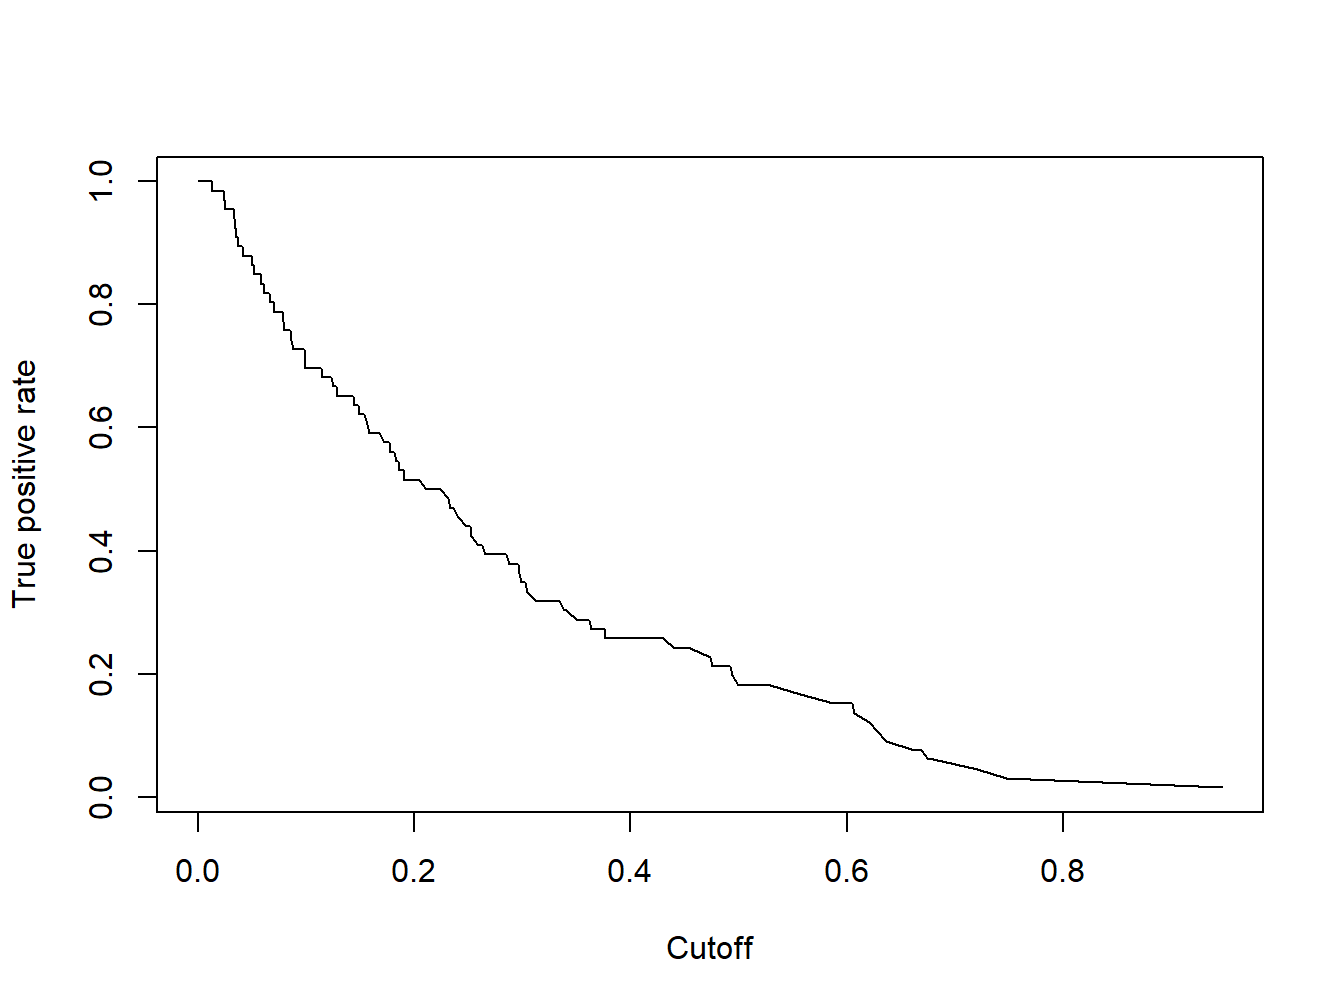
\includegraphics[width=0.8\linewidth]{_main_files/figure-latex/unnamed-chunk-59-1} \end{center}

Los 4 métodos se comportan de forma similar en términos de precisión. Como se ha fijado una semilla y todos los subconjuntos donde se han ajustado los modelos son iguales, es posible hacer inferencias sobre las diferencias entre modelos. Vamos a calcular las diferencias (2 a 2) y luego hacer un t-test bajo la hipótesis nula de que no hay diferencias entre modelos.

\begin{Shaded}
\begin{Highlighting}[]
\NormalTok{difValues <-}\StringTok{ }\KeywordTok{diff}\NormalTok{(resamps)}
\NormalTok{difValues}
\end{Highlighting}
\end{Shaded}

\begin{verbatim}
## 
## Call:
## diff.resamples(x = resamps)
## 
## Models: LDA, QDA, RDA, KNN 
## Metrics: Accuracy, Kappa 
## Number of differences: 6 
## p-value adjustment: bonferroni
\end{verbatim}

\begin{Shaded}
\begin{Highlighting}[]
\KeywordTok{summary}\NormalTok{(difValues)}
\end{Highlighting}
\end{Shaded}

\begin{verbatim}
## 
## Call:
## summary.diff.resamples(object = difValues)
## 
## p-value adjustment: bonferroni 
## Upper diagonal: estimates of the difference
## Lower diagonal: p-value for H0: difference = 0
## 
## Accuracy 
##     LDA     QDA        RDA        KNN       
## LDA         -0.0001247 -0.0001247 -0.0007997
## QDA 1.00000             0.0000000 -0.0006750
## RDA 1.00000 NA                    -0.0006750
## KNN 0.03606 0.06672    0.06672              
## 
## Kappa 
##     LDA       QDA       RDA       KNN     
## LDA           -0.02561  -0.02561  -0.08758
## QDA 0.0001052            0.00000  -0.06197
## RDA 0.0001052 NA                  -0.06197
## KNN 1.406e-13 8.481e-11 8.481e-11
\end{verbatim}

Los resultados indican lo que sospechábamos: no hay diferencias significativas entre los modelos, salvo tal vez entre \emph{LDA} y \emph{KNN} (p-valor \(> 0.05\)). En estos casos, hacer un diagrama con los intervalos de confianza es muy ilustrativo.

\begin{Shaded}
\begin{Highlighting}[]
\CommentTok{# intervalos de confianza para las diferencias}
\KeywordTok{dotplot}\NormalTok{(difValues)}
\end{Highlighting}
\end{Shaded}

\begin{center}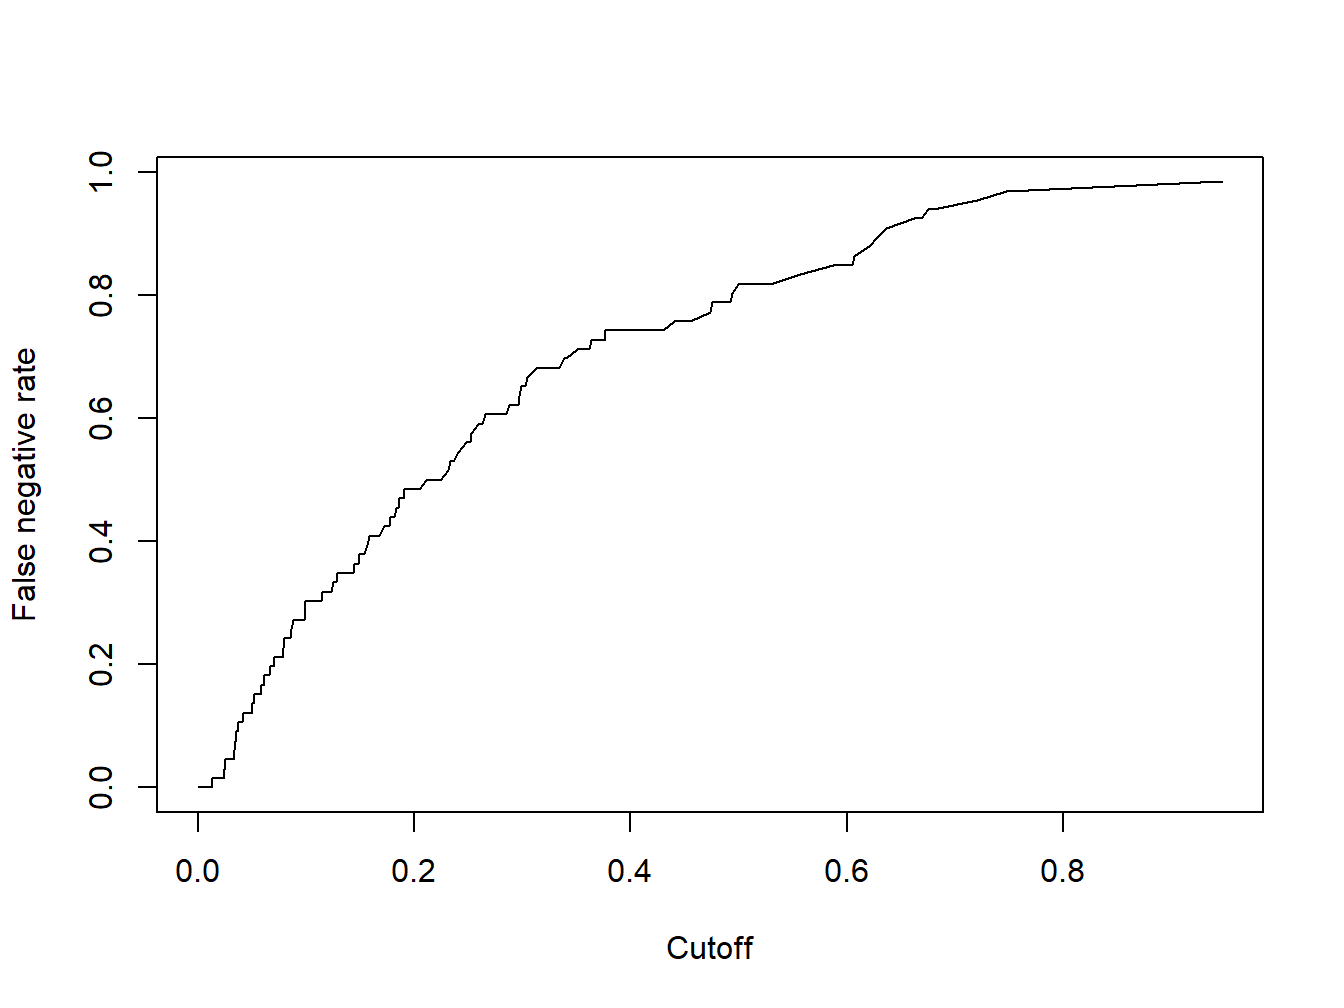
\includegraphics[width=0.8\linewidth]{_main_files/figure-latex/unnamed-chunk-61-1} \end{center}

Solo el intervalo de confianza para la diferencia entre LDA y KNN no contiene al cero, por tanto, hay diferencias significativas para el nivel de confianza fijado.

\hypertarget{curva-roc}{%
\section{\texorpdfstring{Curva \emph{ROC}}{Curva ROC}}\label{curva-roc}}

\hypertarget{anuxe1lisis-en-la-muestra-test}{%
\subsection{Análisis en la muestra test}\label{anuxe1lisis-en-la-muestra-test}}

Hasta ahora solo hemos estudiado la precisión de los modelos usando el \texttt{Accuracy}, pero hay un gran número de medidas cuya aplicación está estrechamente ligada a la naturaleza del problema. Por ejemplo, el clasificador de Bayes asigna una observación a la clase con mayor probabilidad \emph{a posteriori} \(p_k(X)\). Para el problema de los datos \texttt{Default}, donde solo tenemos las clases \texttt{Yes} (el cliente falla en el pago de su tarjeta de crédito) y \texttt{No} (el cliente no falla en el pago), asignamos una observación a la clase \texttt{Yes} si se cumple: \[ \Pr (\text{ default = Yes} | X = x) > 0.5. \]

Pero seguramente el interés del banco es asignar la clase correcta a los malos pagadores y así obtener ganancias, denegando créditos. Esto puede lograrse bajando este \textbf{umbral} de \(0.5\) a \(0.2\), o sea, asignamos una observación a la clase \texttt{Yes} si: \[ \Pr (\text{ default = Yes} | X = x) > 0.2. \]

Decisiones como estas deben basarse en la experiencia de expertos (e.g.~el banco que aprueba el crédito). Vamos a estudiar los tipos de errores que se comenten al variar el umbral de decisión. Para ello, empezamos estimando las probabilidades a posteriori del método LDA en nuestra muestra test:

\begin{Shaded}
\begin{Highlighting}[]
\CommentTok{# hagamos las predicciones del conjunto de prueba}
\NormalTok{pred_prob <-}\StringTok{ }\KeywordTok{predict}\NormalTok{(model_lda_def, }\DataTypeTok{newdata =}\NormalTok{ test_df, }\DataTypeTok{type =} \StringTok{"prob"}\NormalTok{)}
\end{Highlighting}
\end{Shaded}

Usamos el paquete \texttt{ROCR} (Sing et al. \protect\hyperlink{ref-R-ROCR}{2015}) para calcular la Curva \emph{\textbf{R}eceiver \textbf{O}perating \textbf{C}haracteristic} (\emph{ROC}) que compara simultáneamente dos tipos de errores: la \emph{Razón de Falsos Positivos} (\emph{FPR}, siglas en inglés) y la \emph{Razón de Verdaderos Positivos} (\emph{TPR}, siglas en inglés), para un grid de valores del umbral.

\begin{Shaded}
\begin{Highlighting}[]
\KeywordTok{library}\NormalTok{(ROCR)}
\KeywordTok{library}\NormalTok{(dplyr)}

\NormalTok{prob.pred <-}\StringTok{ }\KeywordTok{prediction}\NormalTok{(pred_prob[,}\DecValTok{2}\NormalTok{], test_df}\OperatorTok{$}\NormalTok{default)}

\CommentTok{# ROC}
\NormalTok{prob.pred }\OperatorTok
\StringTok{  }\KeywordTok{performance}\NormalTok{(}\DataTypeTok{measure =} \StringTok{"tpr"}\NormalTok{, }\DataTypeTok{x.measure =} \StringTok{"fpr"}\NormalTok{) }\OperatorTok
\StringTok{  }\KeywordTok{plot}\NormalTok{()}
\end{Highlighting}
\end{Shaded}

\begin{center}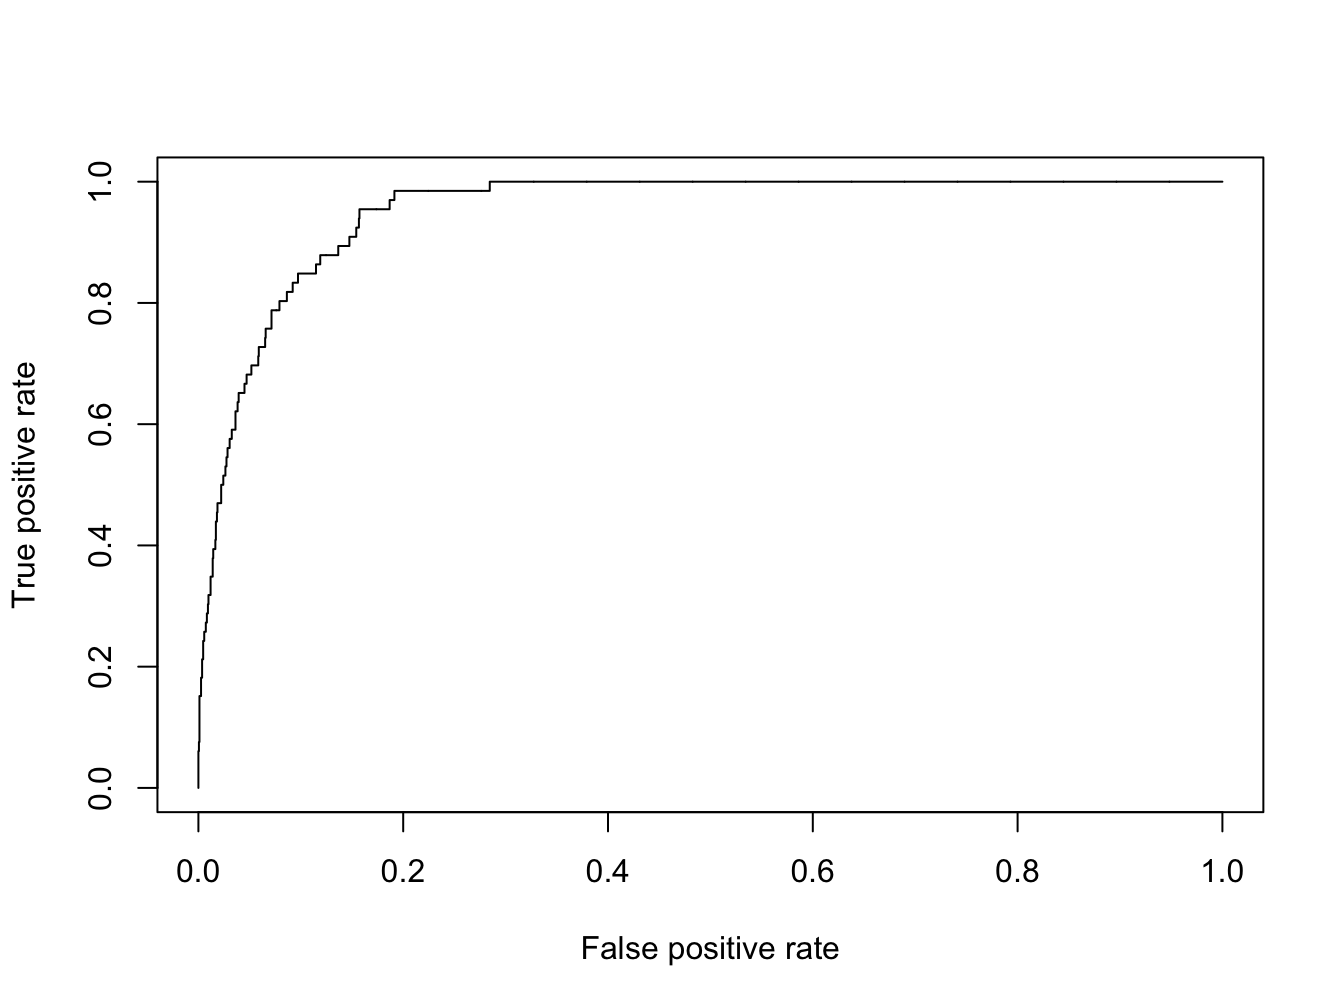
\includegraphics[width=0.8\linewidth]{_main_files/figure-latex/unnamed-chunk-63-1} \end{center}

\begin{Shaded}
\begin{Highlighting}[]
\CommentTok{# AUC: mientras mas cercano a 1, mejor predicciones}
\NormalTok{auc.lda <-}\StringTok{ }\KeywordTok{performance}\NormalTok{(prob.pred, }\DataTypeTok{measure =} \StringTok{"auc"}\NormalTok{)}\OperatorTok{@}\NormalTok{y.values[[}\DecValTok{1}\NormalTok{]]}
\NormalTok{auc.lda}
\end{Highlighting}
\end{Shaded}

\begin{verbatim}
## [1] 0.9526643
\end{verbatim}

El \emph{Área bajo la Curva ROC} (\emph{AUC}, siglas en inglés) resume el rendimiento del clasificador, para todos los posibles umbrales. Una curva ROC ideal debería alcanzar el borde superior izquierdo, por tanto, mientras más cercano a 1 esté el AUC, mejor será. En nuestro ejemplo el área es de \(0.95\), lo cual indica muy buen ajuste. Por otro lado, un AUC cercano a 0.5 indica que el clasificador asigna las clases al azar.

Con el mismo paquete podemos representar otras curvas. Por ejemplo, podemos estudiar por separado, y para diferentes umbrales:

\begin{enumerate}
\def\labelenumi{\arabic{enumi}.}
\tightlist
\item
  La \emph{tasa de error} general para diferentes umbrales: \[ \Pr (\hat{Y} \neq Y) \approx (FP + FN)/(P+N); \]
  donde FP: Falsos Positivos, FN: False Negativos, P: Positivos en la muestra (reales) y N: Negativos en la muestra (reales).
\end{enumerate}

\begin{Shaded}
\begin{Highlighting}[]
\NormalTok{prob.pred }\OperatorTok
\StringTok{  }\KeywordTok{performance}\NormalTok{(}\StringTok{"err"}\NormalTok{) }\OperatorTok
\StringTok{  }\KeywordTok{plot}\NormalTok{()}
\end{Highlighting}
\end{Shaded}

\begin{center}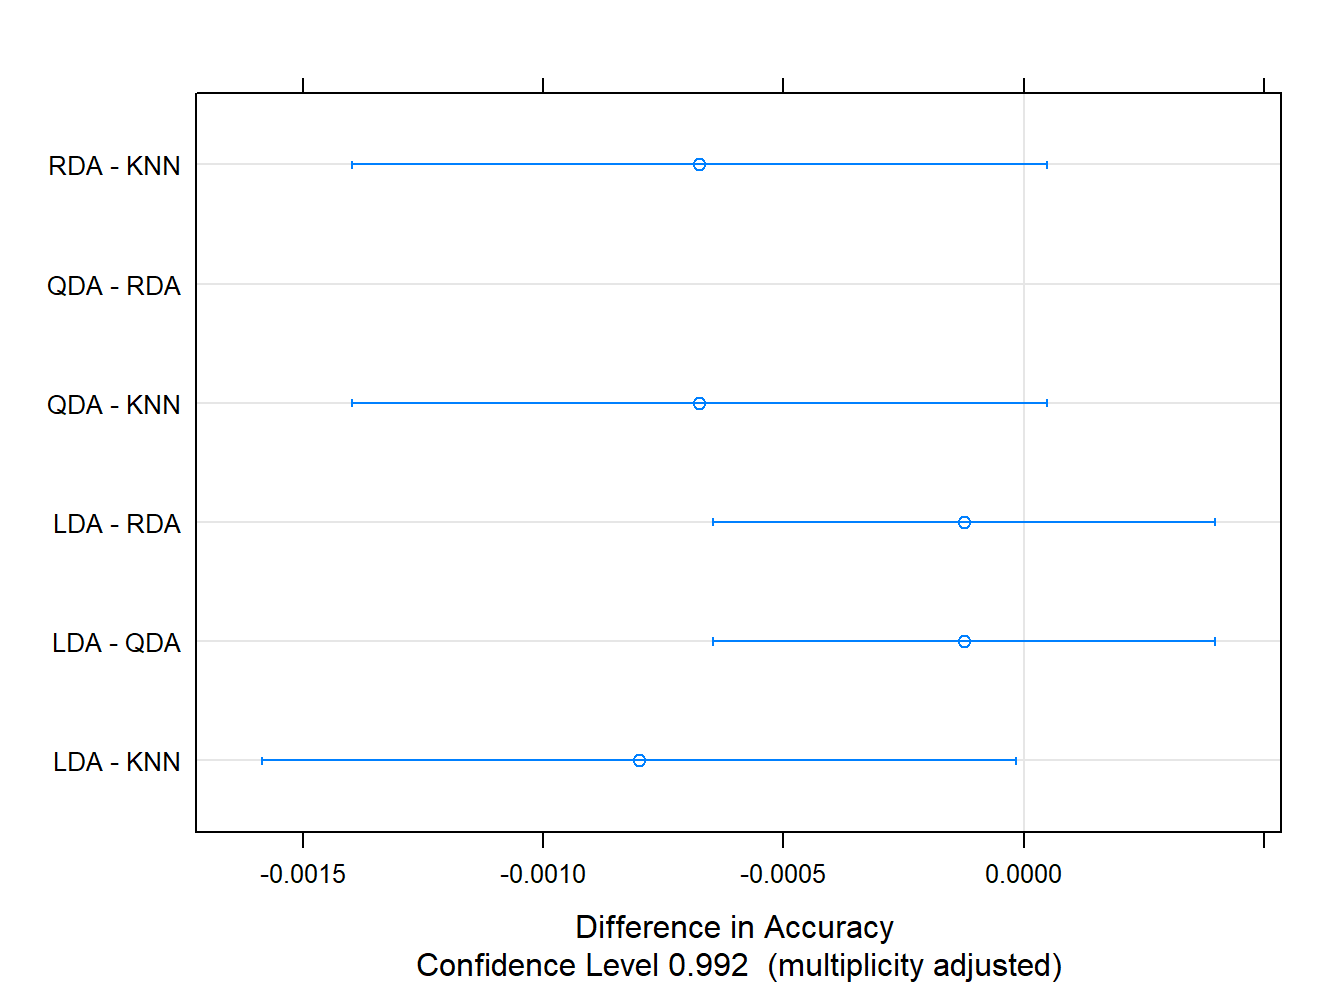
\includegraphics[width=0.8\linewidth]{_main_files/figure-latex/unnamed-chunk-64-1} \end{center}

\begin{enumerate}
\def\labelenumi{\arabic{enumi}.}
\setcounter{enumi}{1}
\tightlist
\item
  La \emph{Razón de Verdaderos Positivos}: \[ P(\hat Y = + | Y = +) \approx TP/P;\]
\end{enumerate}

\begin{Shaded}
\begin{Highlighting}[]
\NormalTok{prob.pred }\OperatorTok
\StringTok{  }\KeywordTok{performance}\NormalTok{(}\StringTok{"tpr"}\NormalTok{) }\OperatorTok
\StringTok{  }\KeywordTok{plot}\NormalTok{()}
\end{Highlighting}
\end{Shaded}

\begin{center}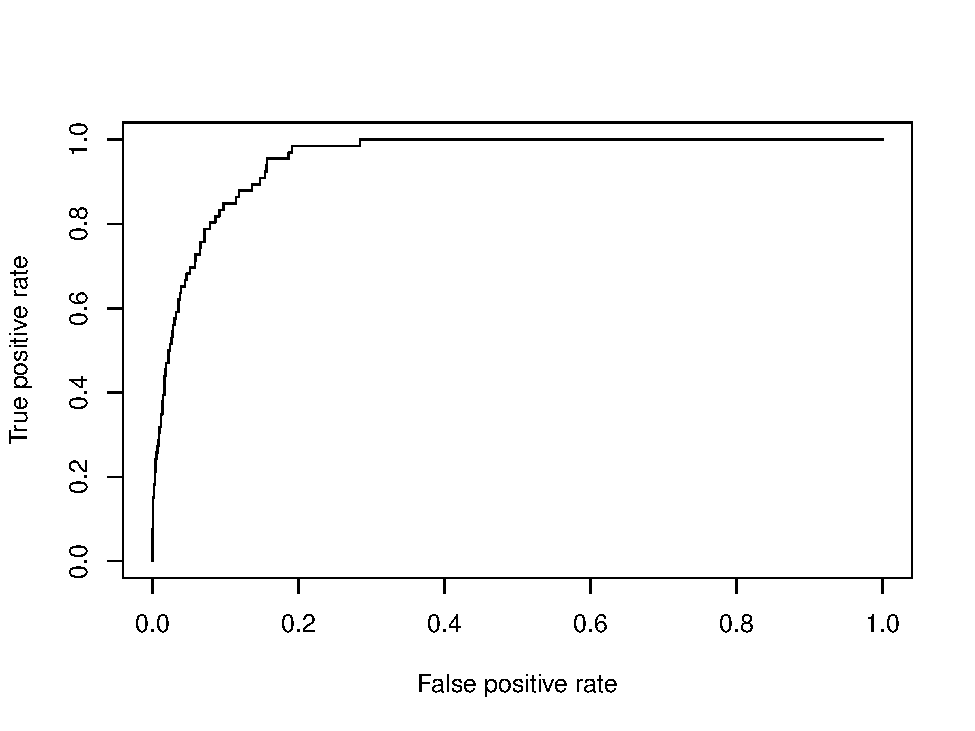
\includegraphics[width=0.8\linewidth]{_main_files/figure-latex/unnamed-chunk-65-1} \end{center}

\begin{enumerate}
\def\labelenumi{\arabic{enumi}.}
\setcounter{enumi}{2}
\tightlist
\item
  La \emph{Razón de Falsos Positivos}: \[ \Pr(\hat Y = + | Y = -) \approx FP/N;\]
\end{enumerate}

\begin{Shaded}
\begin{Highlighting}[]
\NormalTok{prob.pred }\OperatorTok
\StringTok{  }\KeywordTok{performance}\NormalTok{(}\StringTok{"fpr"}\NormalTok{) }\OperatorTok
\StringTok{  }\KeywordTok{plot}\NormalTok{()}
\end{Highlighting}
\end{Shaded}

\begin{center}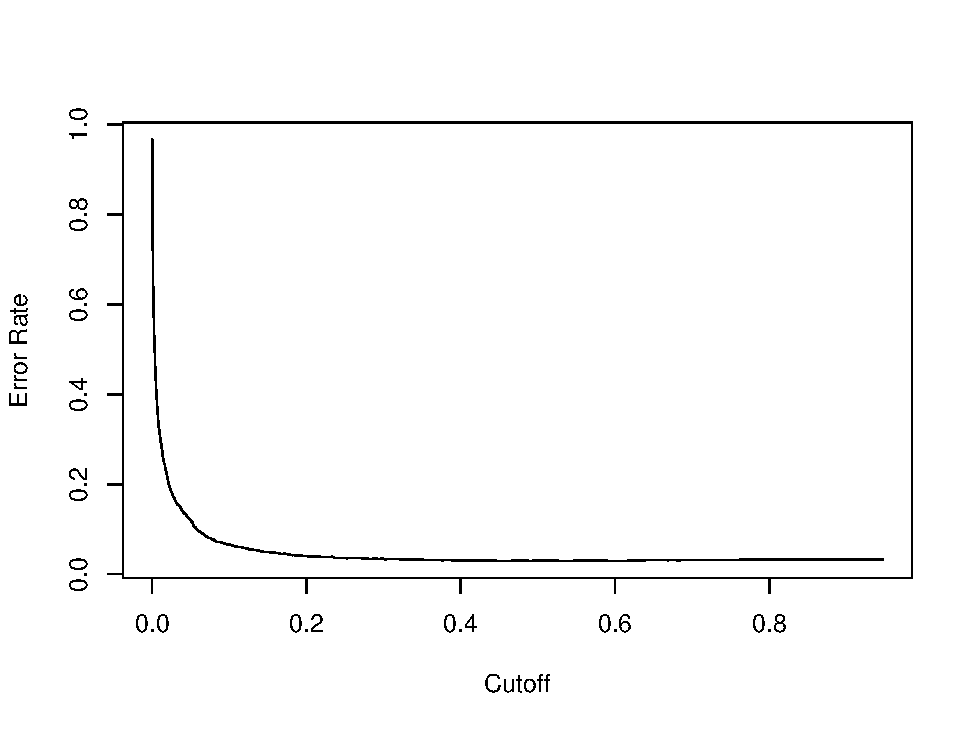
\includegraphics[width=0.8\linewidth]{_main_files/figure-latex/unnamed-chunk-66-1} \end{center}

\begin{enumerate}
\def\labelenumi{\arabic{enumi}.}
\setcounter{enumi}{3}
\tightlist
\item
  La \emph{Razón de Falsos Negativos}: \[ \Pr(\hat Y = - | Y = +) \approx FN/P;\]
\end{enumerate}

\begin{Shaded}
\begin{Highlighting}[]
\NormalTok{prob.pred }\OperatorTok
\StringTok{  }\KeywordTok{performance}\NormalTok{(}\StringTok{"fnr"}\NormalTok{) }\OperatorTok
\StringTok{  }\KeywordTok{plot}\NormalTok{()}
\end{Highlighting}
\end{Shaded}

\begin{center}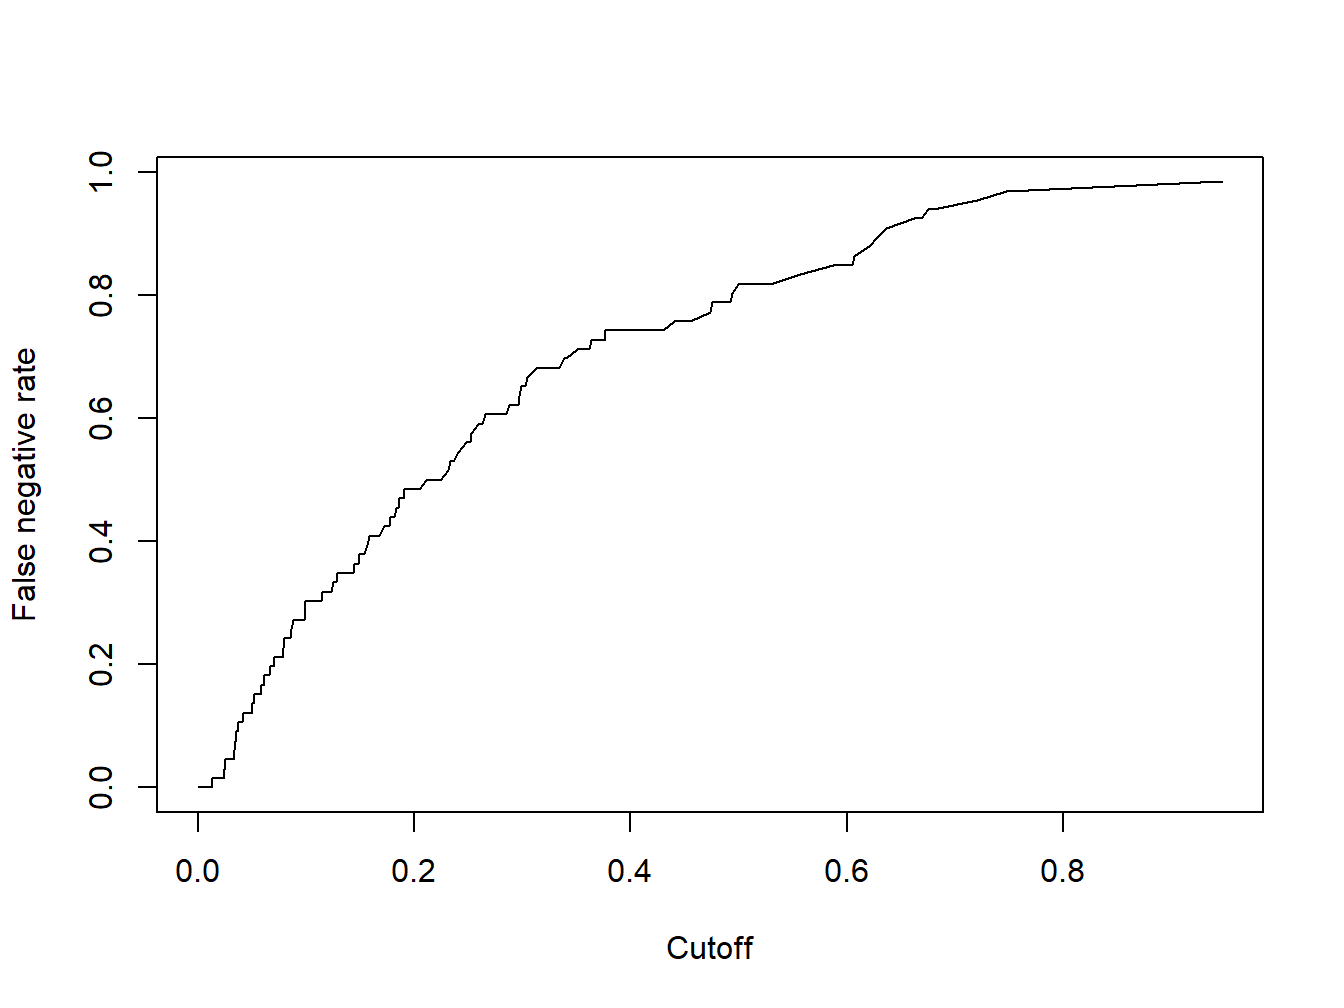
\includegraphics[width=0.8\linewidth]{_main_files/figure-latex/unnamed-chunk-67-1} \end{center}

Toda la información sobre los errores podemos representarla en un mismo gráfico y así ver el equilibrio entre error y umbral:

\begin{Shaded}
\begin{Highlighting}[]
\CommentTok{# Podemos combinar las 3 ultimas en un mismo grafico}
\NormalTok{df_perfor <-}\StringTok{ }\KeywordTok{data.frame}\NormalTok{(}\DataTypeTok{Error.Rate =} \KeywordTok{performance}\NormalTok{(prob.pred, }\StringTok{"err"}\NormalTok{)}\OperatorTok{@}\NormalTok{y.values[[}\DecValTok{1}\NormalTok{]],}
                        \DataTypeTok{FNR =} \KeywordTok{performance}\NormalTok{(prob.pred, }\StringTok{"fnr"}\NormalTok{)}\OperatorTok{@}\NormalTok{y.values[[}\DecValTok{1}\NormalTok{]],}
                        \DataTypeTok{FPR =} \KeywordTok{performance}\NormalTok{(prob.pred, }\StringTok{"fpr"}\NormalTok{)}\OperatorTok{@}\NormalTok{y.values[[}\DecValTok{1}\NormalTok{]],}
                        \DataTypeTok{TPR =} \KeywordTok{performance}\NormalTok{(prob.pred, }\StringTok{"tpr"}\NormalTok{)}\OperatorTok{@}\NormalTok{y.values[[}\DecValTok{1}\NormalTok{]],}
                        \DataTypeTok{CutOffs =} \KeywordTok{performance}\NormalTok{(prob.pred, }\StringTok{"err"}\NormalTok{)}\OperatorTok{@}\NormalTok{x.values[[}\DecValTok{1}\NormalTok{]])}

\CommentTok{# plot tasas de error}
\NormalTok{errores.lda <-}\StringTok{ }\KeywordTok{ggplot}\NormalTok{(df_perfor, }\KeywordTok{aes}\NormalTok{(}\DataTypeTok{x =}\NormalTok{ CutOffs)) }\OperatorTok{+}
\StringTok{  }\KeywordTok{geom_line}\NormalTok{(}\KeywordTok{aes}\NormalTok{(}\DataTypeTok{y =}\NormalTok{ Error.Rate, }\DataTypeTok{colour =} \StringTok{"Tasa Error General"}\NormalTok{)) }\OperatorTok{+}
\StringTok{  }\KeywordTok{geom_line}\NormalTok{(}\KeywordTok{aes}\NormalTok{(}\DataTypeTok{y =}\NormalTok{ FNR, }\DataTypeTok{colour =} \StringTok{"FNR"}\NormalTok{)) }\OperatorTok{+}
\StringTok{  }\KeywordTok{geom_line}\NormalTok{(}\KeywordTok{aes}\NormalTok{(}\DataTypeTok{y =}\NormalTok{ FPR, }\DataTypeTok{colour =} \StringTok{"FPR"}\NormalTok{)) }\OperatorTok{+}
\StringTok{  }\KeywordTok{scale_colour_discrete}\NormalTok{(}\DataTypeTok{name =} \StringTok{"Medidas"}\NormalTok{ ) }\OperatorTok{+}
\StringTok{  }\KeywordTok{xlab}\NormalTok{(}\StringTok{"Puntos de corte"}\NormalTok{) }\OperatorTok{+}\StringTok{ }\KeywordTok{ylab}\NormalTok{(}\StringTok{"Tasas de Error"}\NormalTok{) }\OperatorTok{+}
\StringTok{  }\KeywordTok{theme_light}\NormalTok{()}
\NormalTok{errores.lda}
\end{Highlighting}
\end{Shaded}

\begin{center}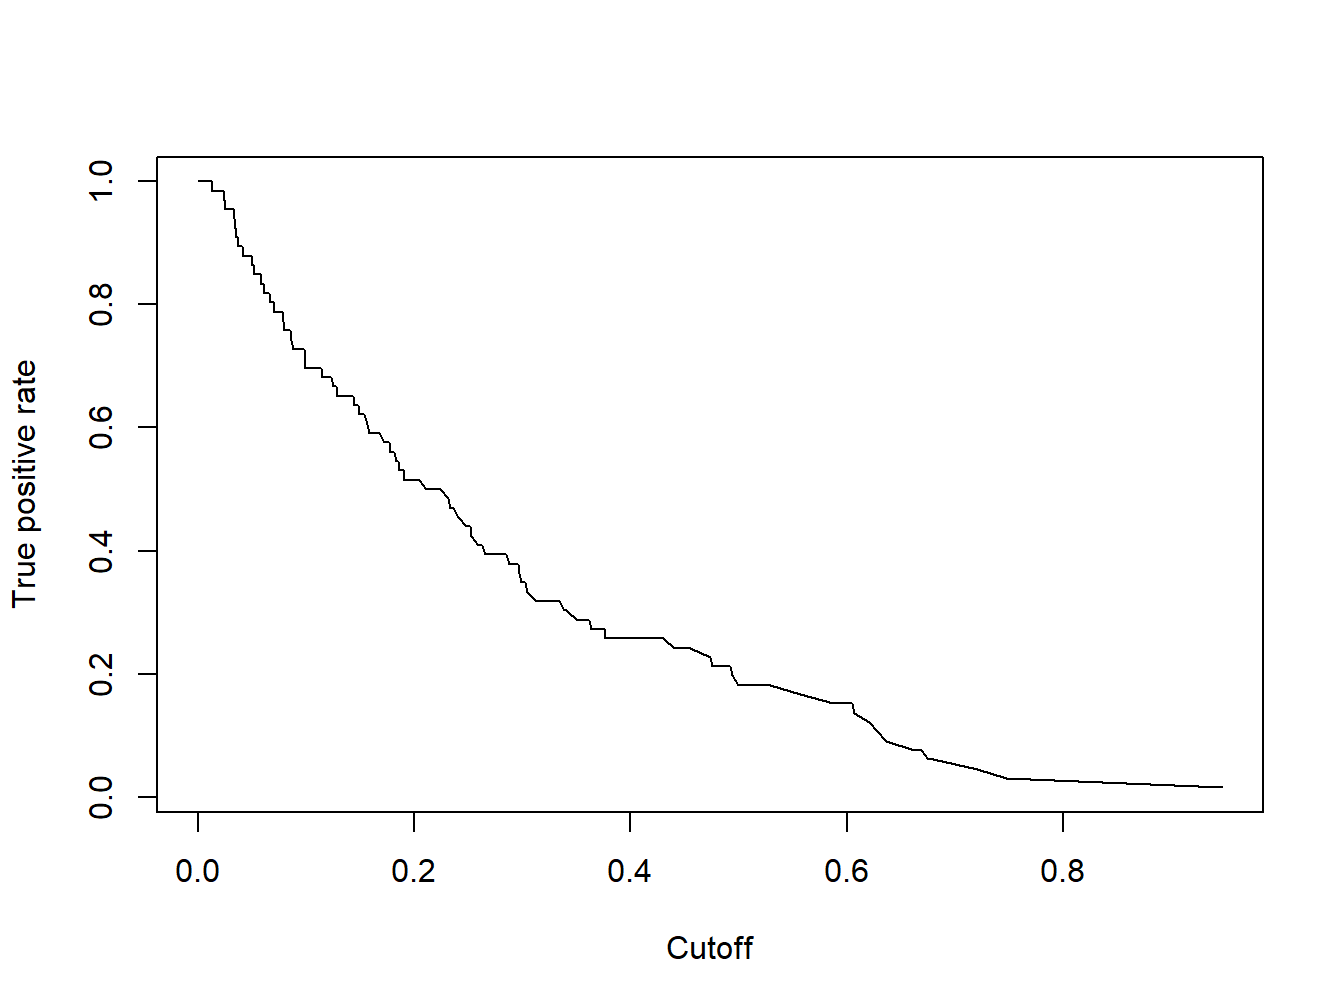
\includegraphics[width=0.8\linewidth]{_main_files/figure-latex/unnamed-chunk-68-1} \end{center}

La curva ROC podemos hacerla en \texttt{ggplot} como se muestra a continuación:

\begin{Shaded}
\begin{Highlighting}[]
\CommentTok{# plot de la curva ROC}
\NormalTok{roc.lda <-}\StringTok{ }\KeywordTok{ggplot}\NormalTok{(df_perfor, }\KeywordTok{aes}\NormalTok{(}\DataTypeTok{x =}\NormalTok{ FPR, }\DataTypeTok{y =}\NormalTok{ TPR)) }\OperatorTok{+}
\StringTok{  }\KeywordTok{geom_line}\NormalTok{() }\OperatorTok{+}
\StringTok{  }\KeywordTok{xlab}\NormalTok{(}\StringTok{"FPR: 1- especificidad"}\NormalTok{) }\OperatorTok{+}\StringTok{ }\KeywordTok{ylab}\NormalTok{(}\StringTok{"TPR: sensibilidad"}\NormalTok{) }\OperatorTok{+}
\StringTok{  }\KeywordTok{ggtitle}\NormalTok{(}\KeywordTok{paste0}\NormalTok{(}\StringTok{"Curva ROC - LDA (Area Under Curve = "}\NormalTok{, }\KeywordTok{round}\NormalTok{(auc.lda, }\DataTypeTok{digits =} \DecValTok{3}\NormalTok{),}\StringTok{")"}\NormalTok{)) }\OperatorTok{+}
\StringTok{  }\KeywordTok{theme_light}\NormalTok{()}
\NormalTok{roc.lda}
\end{Highlighting}
\end{Shaded}

\begin{center}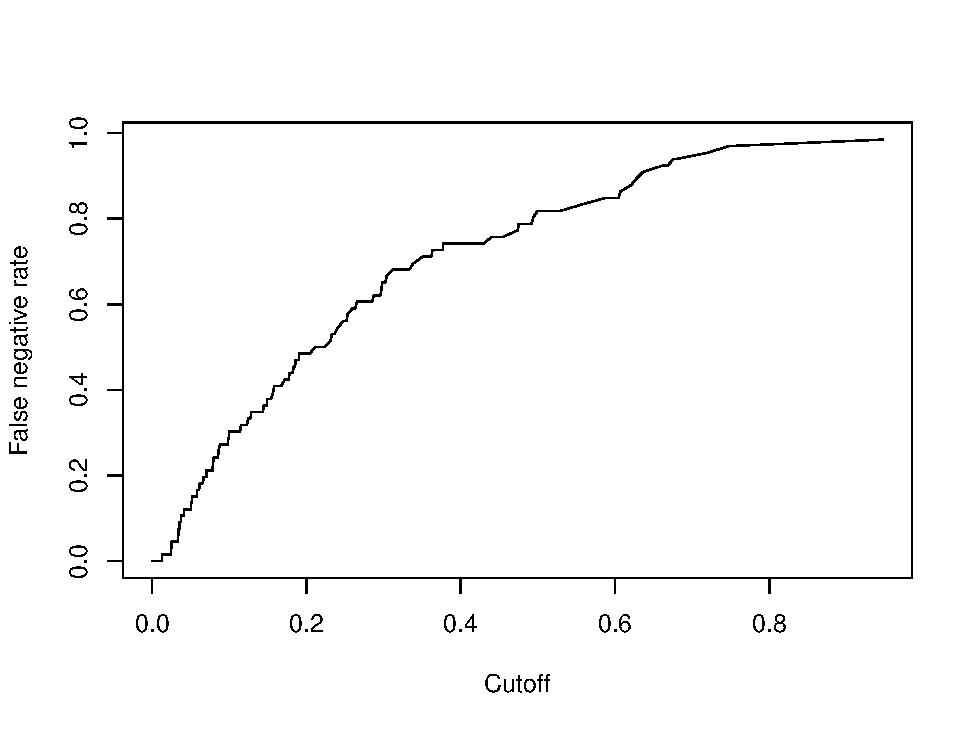
\includegraphics[width=0.8\linewidth]{_main_files/figure-latex/unnamed-chunk-69-1} \end{center}

\hypertarget{anuxe1lisis-en-la-muestra-de-entrenamiento}{%
\subsection{Análisis en la muestra de entrenamiento}\label{anuxe1lisis-en-la-muestra-de-entrenamiento}}

Por defecto, \texttt{caret} calcula el \texttt{RMSE}, el \texttt{MAE} y el \texttt{R\^{}2} como medidas de precisión en el caso de la regresión. En problemas de clasificación, por defecto se computa \texttt{Accuracy} y \texttt{Kappa}, como hemos visto hasta ahora. En el caso de la estimación de los parámetros, se emplea \texttt{RMSE} y \texttt{Accuracy} por defecto. De hecho, el argumento \texttt{metric} de la función \texttt{train} permite al usuario el criterio que desee.

En el caso de clasificación binaria es posible emplear las curvas ROC para comparar el rendimiento entre modelos, justo como hicimos con el \texttt{Accuracy}. Ahora, en lugar de estimar la clase correspondiente, es necesario calcular las probabilidades de cada clase (hacer \texttt{classProbs\ =\ T} en el \texttt{trainControl}) y debemos agregar la opción \texttt{summaryFunction\ =\ twoClassSummary}:

\begin{Shaded}
\begin{Highlighting}[]
\CommentTok{# definimos como control una validación cruzada con 10 hojas y repeticiones}
\NormalTok{fit_control <-}\StringTok{ }\KeywordTok{trainControl}\NormalTok{(}\DataTypeTok{method =} \StringTok{"repeatedcv"}\NormalTok{,}
                           \DataTypeTok{number =} \DecValTok{10}\NormalTok{,}
                           \DataTypeTok{repeats =} \DecValTok{5}\NormalTok{,}
                           \CommentTok{## Estimar las probabilidades:}
                           \DataTypeTok{classProbs =} \OtherTok{TRUE}\NormalTok{,}
                           \CommentTok{## Evaluar rendimiento del modelo:}
                           \DataTypeTok{summaryFunction =}\NormalTok{ twoClassSummary)}

\CommentTok{# LDA}
\KeywordTok{set.seed}\NormalTok{(}\DecValTok{321}\NormalTok{)}
\NormalTok{model_lda_def <-}\StringTok{ }\KeywordTok{train}\NormalTok{(default }\OperatorTok{~}\NormalTok{.,}
                       \DataTypeTok{data =}\NormalTok{ train_df,}
                       \DataTypeTok{method =} \StringTok{"lda"}\NormalTok{,}
                       \DataTypeTok{trControl =}\NormalTok{ fit_control,}
                       \CommentTok{## Especificamos la métrica para optimizar:}
                       \DataTypeTok{metric =} \StringTok{"ROC"}\NormalTok{)}
\CommentTok{# QDA}
\KeywordTok{set.seed}\NormalTok{(}\DecValTok{321}\NormalTok{)}
\NormalTok{model_qda_def <-}\StringTok{ }\KeywordTok{train}\NormalTok{(default }\OperatorTok{~}\NormalTok{.,}
                       \DataTypeTok{data =}\NormalTok{ train_df,}
                       \DataTypeTok{method =} \StringTok{"qda"}\NormalTok{,}
                       \DataTypeTok{trControl =}\NormalTok{ fit_control,}
                       \CommentTok{## Especificamos la métrica para optimizar:}
                       \DataTypeTok{metric =} \StringTok{"ROC"}\NormalTok{)}

\CommentTok{# RDA}

\NormalTok{mi.grid <-}\StringTok{ }\KeywordTok{data.frame}\NormalTok{(}\DataTypeTok{lambda =} \KeywordTok{c}\NormalTok{(}\DecValTok{0}\NormalTok{) , }
                       \DataTypeTok{gamma =} \KeywordTok{c}\NormalTok{(}\DecValTok{0}\NormalTok{))}

\KeywordTok{set.seed}\NormalTok{(}\DecValTok{321}\NormalTok{)}
\NormalTok{model_rda_def <-}\StringTok{ }\KeywordTok{train}\NormalTok{(default }\OperatorTok{~}\NormalTok{.,}
                       \DataTypeTok{data =}\NormalTok{ train_df,}
                       \DataTypeTok{method =} \StringTok{"rda"}\NormalTok{,}
                       \DataTypeTok{tuneGrid =}\NormalTok{ mi.grid,}
                       \DataTypeTok{trControl =}\NormalTok{ fit_control,}
                       \CommentTok{## Especificamos la métrica para optimizar:}
                       \DataTypeTok{metric =} \StringTok{"ROC"}\NormalTok{)}

\KeywordTok{set.seed}\NormalTok{(}\DecValTok{321}\NormalTok{)}
\NormalTok{model_knn_def <-}\StringTok{ }\KeywordTok{train}\NormalTok{(default }\OperatorTok{~}\NormalTok{.,}
                       \DataTypeTok{data =}\NormalTok{ train_df,}
                       \DataTypeTok{method =} \StringTok{"knn"}\NormalTok{,}
                       \DataTypeTok{trControl =}\NormalTok{ fit_control,}
                       \DataTypeTok{preProcess =} \KeywordTok{c}\NormalTok{(}\StringTok{"center"}\NormalTok{, }\StringTok{"scale"}\NormalTok{),}
                       \DataTypeTok{tuneLength =} \DecValTok{5}\NormalTok{,}
                       \CommentTok{## Especificamos la métrica para optimizar:}
                       \DataTypeTok{metric =} \StringTok{"ROC"}\NormalTok{)}
\NormalTok{model_knn_def}
\end{Highlighting}
\end{Shaded}

\begin{verbatim}
## k-Nearest Neighbors 
## 
## 8001 samples
##    2 predictor
##    2 classes: 'No', 'Yes' 
## 
## Pre-processing: centered (2), scaled (2) 
## Resampling: Cross-Validated (10 fold, repeated 5 times) 
## Summary of sample sizes: 7200, 7200, 7201, 7201, 7201, 7201, ... 
## Resampling results across tuning parameters:
## 
##   k   ROC        Sens       Spec     
##    5  0.7988217  0.9933019  0.3594302
##    7  0.8170610  0.9936381  0.3722792
##    9  0.8328763  0.9947759  0.3684330
##   11  0.8508985  0.9950345  0.3602849
##   13  0.8614489  0.9956036  0.3498575
## 
## ROC was used to select the optimal model using the largest value.
## The final value used for the model was k = 13.
\end{verbatim}

Usamos una vez más la función \texttt{resamples} para agrupar todos los resultados calculados de cada modelo:

\begin{Shaded}
\begin{Highlighting}[]
\NormalTok{resamps <-}\StringTok{ }\KeywordTok{resamples}\NormalTok{(}\KeywordTok{list}\NormalTok{(}\DataTypeTok{LDA =}\NormalTok{ model_lda_def,}
                          \DataTypeTok{QDA =}\NormalTok{ model_qda_def,}
                          \DataTypeTok{RDA =}\NormalTok{ model_rda_def,}
                          \DataTypeTok{KNN =}\NormalTok{ model_knn_def))}
\NormalTok{resamps}
\end{Highlighting}
\end{Shaded}

\begin{verbatim}
## 
## Call:
## resamples.default(x = list(LDA = model_lda_def, QDA = model_qda_def, RDA
##  = model_rda_def, KNN = model_knn_def))
## 
## Models: LDA, QDA, RDA, KNN 
## Number of resamples: 50 
## Performance metrics: ROC, Sens, Spec 
## Time estimates for: everything, final model fit
\end{verbatim}

\begin{Shaded}
\begin{Highlighting}[]
\KeywordTok{summary}\NormalTok{(resamps)}
\end{Highlighting}
\end{Shaded}

\begin{verbatim}
## 
## Call:
## summary.resamples(object = resamps)
## 
## Models: LDA, QDA, RDA, KNN 
## Number of resamples: 50 
## 
## ROC 
##          Min.   1st Qu.    Median      Mean   3rd Qu.      Max. NA's
## LDA 0.8957110 0.9386303 0.9524699 0.9476517 0.9609670 0.9730248    0
## QDA 0.8959100 0.9386739 0.9519189 0.9474556 0.9607047 0.9725936    0
## RDA 0.8959100 0.9386739 0.9519189 0.9474556 0.9607047 0.9725936    0
## KNN 0.7301416 0.8398544 0.8648040 0.8614489 0.8882339 0.9492118    0
## 
## Sens 
##          Min.   1st Qu.    Median      Mean   3rd Qu. Max. NA's
## LDA 0.9948320 0.9974127 0.9980612 0.9981379 0.9996770    1    0
## QDA 0.9935317 0.9961190 0.9974127 0.9973362 0.9987063    1    0
## RDA 0.9935317 0.9961190 0.9974127 0.9973362 0.9987063    1    0
## KNN 0.9909444 0.9948254 0.9961190 0.9956036 0.9970905    1    0
## 
## Spec 
##           Min.   1st Qu.    Median      Mean   3rd Qu.      Max. NA's
## LDA 0.07407407 0.1869658 0.2307692 0.2524786 0.2962963 0.4615385    0
## QDA 0.11111111 0.1997863 0.2642450 0.2794017 0.3333333 0.4814815    0
## RDA 0.11111111 0.1997863 0.2642450 0.2794017 0.3333333 0.4814815    0
## KNN 0.18518519 0.2962963 0.3333333 0.3498575 0.4074074 0.5925926    0
\end{verbatim}

\begin{Shaded}
\begin{Highlighting}[]
\CommentTok{# box plots}
\KeywordTok{bwplot}\NormalTok{(resamps, }\DataTypeTok{metric =} \StringTok{"ROC"}\NormalTok{)}
\end{Highlighting}
\end{Shaded}

\begin{center}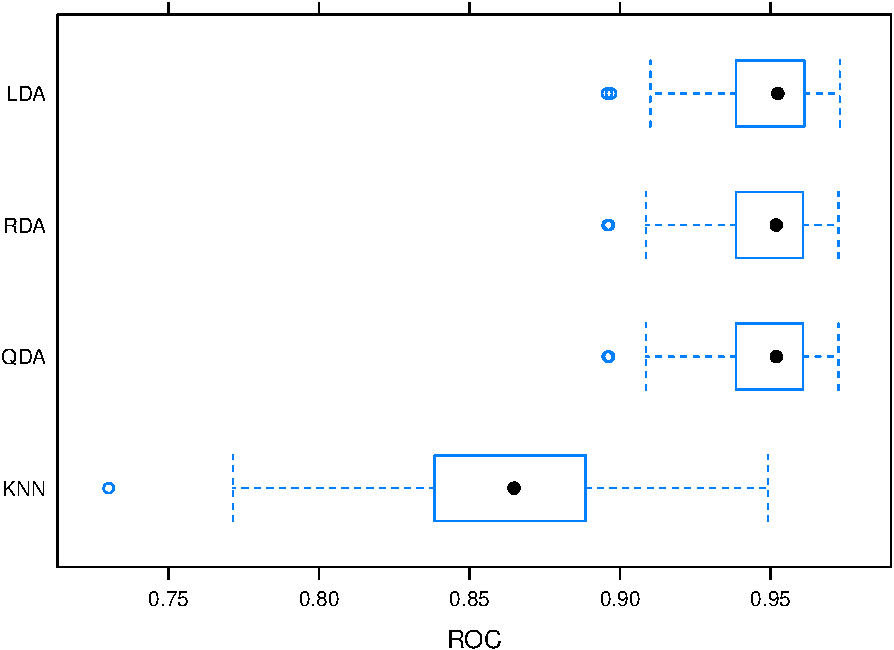
\includegraphics[width=0.8\linewidth]{_main_files/figure-latex/unnamed-chunk-72-1} \end{center}

Los 3 métodos Discriminantes se comportan de forma similar, lo cual es de esperar ya que los hemos entrenado poco por cuestiones prácticas (¡demoran!). El KNN parece ser el peor de todos, pero tampoco hemos puesto mucho empeño en calcular el número óptimo de vecinos. Aún así, estos valores de AUC son muy buenos, en la práctica es difícil conseguir estos resultados.

Pasamos a hacer algunas inferencias. Particularmente, vamos a calcular las diferencias (2 a 2) y luego hacer un t-test bajo la hipótesis nula de que no hay diferencias entre modelos.

\begin{Shaded}
\begin{Highlighting}[]
\NormalTok{difValues <-}\StringTok{ }\KeywordTok{diff}\NormalTok{(resamps)}
\NormalTok{difValues}
\end{Highlighting}
\end{Shaded}

\begin{verbatim}
## 
## Call:
## diff.resamples(x = resamps)
## 
## Models: LDA, QDA, RDA, KNN 
## Metrics: ROC, Sens, Spec 
## Number of differences: 6 
## p-value adjustment: bonferroni
\end{verbatim}

\begin{Shaded}
\begin{Highlighting}[]
\KeywordTok{summary}\NormalTok{(difValues)}
\end{Highlighting}
\end{Shaded}

\begin{verbatim}
## 
## Call:
## summary.diff.resamples(object = difValues)
## 
## p-value adjustment: bonferroni 
## Upper diagonal: estimates of the difference
## Lower diagonal: p-value for H0: difference = 0
## 
## ROC 
##     LDA     QDA       RDA       KNN      
## LDA         0.0001961 0.0001961 0.0862029
## QDA 0.05335           0.0000000 0.0860067
## RDA 0.05335 NA                  0.0860067
## KNN < 2e-16 < 2e-16   < 2e-16            
## 
## Sens 
##     LDA       QDA       RDA       KNN      
## LDA           0.0008017 0.0008017 0.0025343
## QDA 4.441e-06           0.0000000 0.0017326
## RDA 4.441e-06 NA                  0.0017326
## KNN 1.367e-12 1.261e-08 1.261e-08          
## 
## Spec 
##     LDA       QDA       RDA       KNN     
## LDA           -0.02692  -0.02692  -0.09738
## QDA 1.942e-07            0.00000  -0.07046
## RDA 1.942e-07 NA                  -0.07046
## KNN < 2.2e-16 9.408e-14 9.408e-14
\end{verbatim}

Los resultados indican lo que sospechábamos: hay diferencias significativas entre los modelos \emph{(X)DA} y el \emph{KNN} (p-valor \(> 0.05\)). En estos casos, hacer un diagrama con los intervalos de confianza es mucho más ilustrativo.

\begin{Shaded}
\begin{Highlighting}[]
\CommentTok{# intervalos de confianza para las diferencias}
\KeywordTok{dotplot}\NormalTok{(difValues)}
\end{Highlighting}
\end{Shaded}

\begin{center}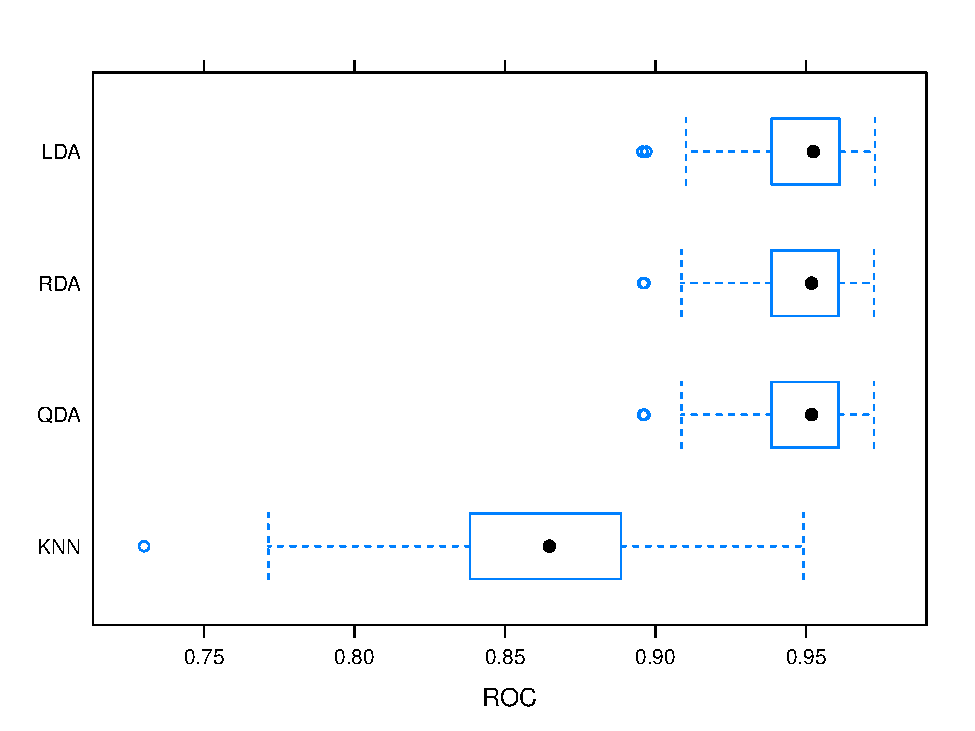
\includegraphics[width=0.8\linewidth]{_main_files/figure-latex/unnamed-chunk-74-1} \end{center}

En la práctica, el siguiente paso sería escoger el modelo más competitivo de acuerdo a alguno de los criterios estudiados y, con este, predecir las respuestas de la muestra test.

\hypertarget{wiscon}{%
\chapter{Wisconsin Breast-Cancer Data}\label{wiscon}}

Los datos de cáncer de mama Wisconsin están disponibles en diversas plataformas. Por ejemplo, en \href{https://www.kaggle.com/uciml/breast-cancer-wisconsin-data}{Kaggle}. Estos corresponden a mediciones obtenidas ``\emph{de una imagen digitalizada de un aspirado con aguja fina (FNA) de una masa mamaria}''. La variables describen las características de los núcleos celulares presentes en la imagen. Este conjunto de datos es muy didáctico y permite estimar si los tumores son malignos o benignos, conociendo la media, desviación estándar y valor máximo de 10 mediciones de cada una de las 10 características:

\begin{itemize}
\tightlist
\item
  radius (mean of distances from center to points on the perimeter)
\item
  texture (standard deviation of gray-scale values)
\item
  perimeter
\item
  area
\item
  smoothness (local variation in radius lengths)
\item
  compactness (perimeter\^{}2 / area - 1.0)
\item
  concavity (severity of concave portions of the contour)
\item
  concave points (number of concave portions of the contour)
\item
  symmetry
\item
  fractal dimension (``coastline approximation'' - 1)
\end{itemize}

El resultado es un problema de clasificación binario (\(Y =\) \texttt{diagnosis}) con 30 variables predictoras. La muestra de 569 pacientes corresponde a 357 en la clase \texttt{B} y 212 en la clase \texttt{M}. Los datos están disponibles en este repositorio y también en Aula Global.

\begin{Shaded}
\begin{Highlighting}[]
\KeywordTok{library}\NormalTok{(caret)}
\KeywordTok{library}\NormalTok{(ggplot2)}
\KeywordTok{library}\NormalTok{(readr)}
\KeywordTok{library}\NormalTok{(dplyr)}
\KeywordTok{library}\NormalTok{(gridExtra)}
\KeywordTok{library}\NormalTok{(ROCR)}

\CommentTok{## Cargar datos ----}
\NormalTok{wiscon <-}\StringTok{ }\KeywordTok{read_csv}\NormalTok{(}\StringTok{"data_breast_cancer_wisconsin.csv"}\NormalTok{)}

\CommentTok{# no nos interesan los ID, y la última columna no se ha cargado bien}
\NormalTok{wiscon <-}\StringTok{ }\NormalTok{wiscon[, }\DecValTok{2}\OperatorTok{:}\DecValTok{32}\NormalTok{]}

\CommentTok{# la respuesta es diagnosis: B = benign, M = malignant}
\NormalTok{wiscon}\OperatorTok{$}\NormalTok{diagnosis <-}\StringTok{ }\KeywordTok{as.factor}\NormalTok{(wiscon}\OperatorTok{$}\NormalTok{diagnosis)}

\NormalTok{df <-}\StringTok{ }\KeywordTok{as.data.frame}\NormalTok{(wiscon)}

\KeywordTok{str}\NormalTok{(df)}
\end{Highlighting}
\end{Shaded}

\begin{verbatim}
## 'data.frame':    569 obs. of  31 variables:
##  $ diagnosis              : Factor w/ 2 levels "B","M": 2 2 2 2 2 2 2 2 2 2 ...
##  $ radius_mean            : num  18 20.6 19.7 11.4 20.3 ...
##  $ texture_mean           : num  10.4 17.8 21.2 20.4 14.3 ...
##  $ perimeter_mean         : num  122.8 132.9 130 77.6 135.1 ...
##  $ area_mean              : num  1001 1326 1203 386 1297 ...
##  $ smoothness_mean        : num  0.1184 0.0847 0.1096 0.1425 0.1003 ...
##  $ compactness_mean       : num  0.2776 0.0786 0.1599 0.2839 0.1328 ...
##  $ concavity_mean         : num  0.3001 0.0869 0.1974 0.2414 0.198 ...
##  $ concave points_mean    : num  0.1471 0.0702 0.1279 0.1052 0.1043 ...
##  $ symmetry_mean          : num  0.242 0.181 0.207 0.26 0.181 ...
##  $ fractal_dimension_mean : num  0.0787 0.0567 0.06 0.0974 0.0588 ...
##  $ radius_se              : num  1.095 0.543 0.746 0.496 0.757 ...
##  $ texture_se             : num  0.905 0.734 0.787 1.156 0.781 ...
##  $ perimeter_se           : num  8.59 3.4 4.58 3.44 5.44 ...
##  $ area_se                : num  153.4 74.1 94 27.2 94.4 ...
##  $ smoothness_se          : num  0.0064 0.00522 0.00615 0.00911 0.01149 ...
##  $ compactness_se         : num  0.049 0.0131 0.0401 0.0746 0.0246 ...
##  $ concavity_se           : num  0.0537 0.0186 0.0383 0.0566 0.0569 ...
##  $ concave points_se      : num  0.0159 0.0134 0.0206 0.0187 0.0188 ...
##  $ symmetry_se            : num  0.03 0.0139 0.0225 0.0596 0.0176 ...
##  $ fractal_dimension_se   : num  0.00619 0.00353 0.00457 0.00921 0.00511 ...
##  $ radius_worst           : num  25.4 25 23.6 14.9 22.5 ...
##  $ texture_worst          : num  17.3 23.4 25.5 26.5 16.7 ...
##  $ perimeter_worst        : num  184.6 158.8 152.5 98.9 152.2 ...
##  $ area_worst             : num  2019 1956 1709 568 1575 ...
##  $ smoothness_worst       : num  0.162 0.124 0.144 0.21 0.137 ...
##  $ compactness_worst      : num  0.666 0.187 0.424 0.866 0.205 ...
##  $ concavity_worst        : num  0.712 0.242 0.45 0.687 0.4 ...
##  $ concave points_worst   : num  0.265 0.186 0.243 0.258 0.163 ...
##  $ symmetry_worst         : num  0.46 0.275 0.361 0.664 0.236 ...
##  $ fractal_dimension_worst: num  0.1189 0.089 0.0876 0.173 0.0768 ...
##  - attr(*, "problems")=Classes 'tbl_df', 'tbl' and 'data.frame': 569 obs. of  5 variables:
##   ..$ row     : int  1 2 3 4 5 6 7 8 9 10 ...
##   ..$ col     : chr  NA NA NA NA ...
##   ..$ expected: chr  "33 columns" "33 columns" "33 columns" "33 columns" ...
##   ..$ actual  : chr  "32 columns" "32 columns" "32 columns" "32 columns" ...
##   ..$ file    : chr  "'data_breast_cancer_wisconsin.csv'" "'data_breast_cancer_wisconsin.csv'" "'data_breast_cancer_wisconsin.csv'" "'data_breast_cancer_wisconsin.csv'" ...
\end{verbatim}

Vamos a crear una partición independiente (con una semilla) de test y aplicar todo lo estudiado hasta ahora.

\begin{Shaded}
\begin{Highlighting}[]
\KeywordTok{set.seed}\NormalTok{(}\DecValTok{666}\NormalTok{)}
\NormalTok{train.ID <-}\StringTok{ }\KeywordTok{createDataPartition}\NormalTok{(df}\OperatorTok{$}\NormalTok{diagnosis, }\DataTypeTok{p =} \FloatTok{0.7}\NormalTok{, }\DataTypeTok{list =} \OtherTok{FALSE}\NormalTok{)}

\NormalTok{train_df <-}\StringTok{ }\NormalTok{df[train.ID, ]}
\NormalTok{test_df <-}\StringTok{ }\NormalTok{df[}\OperatorTok{-}\NormalTok{train.ID, ]}
\end{Highlighting}
\end{Shaded}

¡A por ello!

\hypertarget{comentarios-finales-reducciuxf3n-de-la-dimensiuxf3n}{%
\section{Comentarios finales: reducción de la dimensión}\label{comentarios-finales-reducciuxf3n-de-la-dimensiuxf3n}}

Aunque queda fuera del \emph{aprendizaje supervisado}, como posible solución a la alta dimensionalidad de los datos, en \texttt{caret} es posible aplicar técnicas \emph{no supervisadas} que permiten \emph{reducir la dimensión}. Una de ellas es el \emph{Análisis de Componentes Principales} (\emph{PCA}, por sus siglas en inglés). Veamos cómo hacer esto con la función \texttt{preProcess}:

\begin{Shaded}
\begin{Highlighting}[]
\CommentTok{# en este caso estamos reduciendo la cantidad de variables iniciales}
\CommentTok{# a solamente ¡2!}
\NormalTok{preProc.res <-}\StringTok{ }\KeywordTok{preProcess}\NormalTok{(df, }\DataTypeTok{method =} \KeywordTok{c}\NormalTok{(}\StringTok{'pca'}\NormalTok{), }\DataTypeTok{pcaComp =} \DecValTok{2}\NormalTok{)}
\NormalTok{df.pca <-}\StringTok{ }\KeywordTok{predict}\NormalTok{(preProc.res, df)}

\KeywordTok{head}\NormalTok{(df.pca, }\DecValTok{7}\NormalTok{)}
\end{Highlighting}
\end{Shaded}

\begin{verbatim}
##   diagnosis       PC1        PC2
## 1         M -9.184755  -1.946870
## 2         M -2.385703   3.764859
## 3         M -5.728855   1.074229
## 4         M -7.116691 -10.266556
## 5         M -3.931842   1.946359
## 6         M -2.378155  -3.946456
## 7         M -2.236915   2.687666
\end{verbatim}

Veamos qué tan separadas quedan las clases ahora:

\begin{Shaded}
\begin{Highlighting}[]
\KeywordTok{ggplot}\NormalTok{(df.pca,  }\KeywordTok{aes}\NormalTok{(}\DataTypeTok{x =}\NormalTok{ PC1, }\DataTypeTok{y =}\NormalTok{ PC2, }\DataTypeTok{group =}\NormalTok{ diagnosis)) }\OperatorTok{+}
\StringTok{  }\KeywordTok{geom_point}\NormalTok{(}\KeywordTok{aes}\NormalTok{(}\DataTypeTok{color =}\NormalTok{ diagnosis ), }\DataTypeTok{alpha =} \FloatTok{0.8}\NormalTok{) }\OperatorTok{+}
\StringTok{  }\KeywordTok{theme_light}\NormalTok{()}
\end{Highlighting}
\end{Shaded}

\begin{center}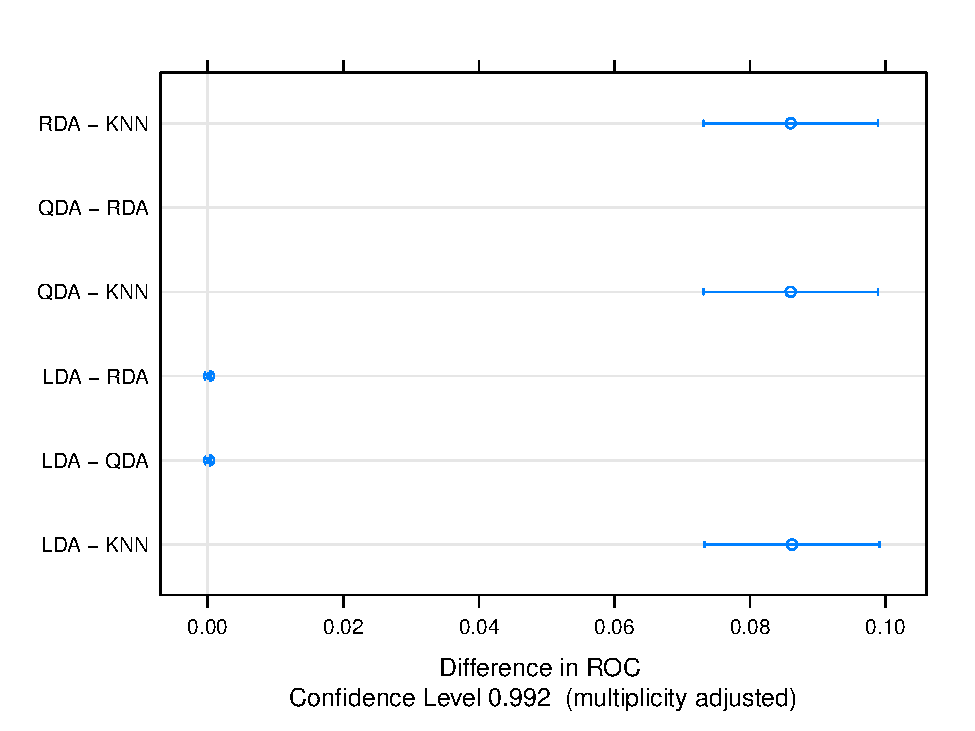
\includegraphics[width=0.8\linewidth]{_main_files/figure-latex/unnamed-chunk-78-1} \end{center}

Si volvemos a hacer la partición de los datos (mismos índices para el test);

\begin{Shaded}
\begin{Highlighting}[]
\CommentTok{# Ajustemos nuestros modelos con los datos transformados:}
\NormalTok{train_df <-}\StringTok{ }\NormalTok{df.pca[train.ID, ]}
\NormalTok{test_df <-}\StringTok{ }\NormalTok{df.pca[}\OperatorTok{-}\NormalTok{train.ID, ]}
\end{Highlighting}
\end{Shaded}

entonces, podemos aplicar todos los modelos estudiados a un conjunto de datos de menor complejidad. Esto es una ganancia en tiempo de cómputo\ldots{} ¿será también en términos predictivos? Intenta también \textbf{representar la frontera de decisión} correspondiente a cada método, usando como base la ya conocida \texttt{decision\_bound}.

Finalmente, comentar que el LDA también puede ser visto como un método de reducción de la dimensión. La visión de Fisher del discriminante lineal contempla encontrar la mejor proyección de los datos (a una dimensión inferior) que permita separar bien las clases. Esto se logra persiguiendo la mayor dispersión posible en los datos.

Más información sobre el PCA puede ser consultada en los libros que se citan al final del documento. Una buena introducción a esta visión del LDA está disponible en las \href{https://www.csd.uwo.ca/~olga/Courses/CS434a_541a/Lecture8.pdf}{lecciones de Prof.~Olga Veksler}. También se recomiendo el excelente \href{https://www.datascienceblog.net/post/machine-learning/linear-discriminant-analysis/}{post de Matthias Döring}.

\hypertarget{refs}{}
\leavevmode\hypertarget{ref-Burger2018}{}%
Burger, Scott V. 2018. \emph{Introduction to machine learning with R - Rigorous mathematical modeling}. Vol. 1. O'Reilly.

\leavevmode\hypertarget{ref-R-ISLR}{}%
James, Gareth, Daniela Witten, Trevor Hastie, and Rob Tibshirani. 2017. \emph{ISLR: Data for an Introduction to Statistical Learning with Applications in R}. \url{https://CRAN.R-project.org/package=ISLR}.

\leavevmode\hypertarget{ref-james2013introduction}{}%
James, Gareth, Daniela Witten, Trevor Hastie, and Robert Tibshirani. 2013. \emph{An Introduction to Statistical Learning with Applications in R*}. Vol. 6. Springer.

\leavevmode\hypertarget{ref-R-caret}{}%
Kuhn, Max. 2020. \emph{Caret: Classification and Regression Training}. \url{https://CRAN.R-project.org/package=caret}.

\leavevmode\hypertarget{ref-Rebala2019}{}%
Rebala, Gopinath, Ajay Ravi, and Sanjay Churiwala. 2019. \emph{An Introduction to Machine Learning}. Cham: Springer International Publishing. \url{https://doi.org/10.1007/978-3-030-15729-6}.

\leavevmode\hypertarget{ref-R-class}{}%
Ripley, Brian. 2019. \emph{Class: Functions for Classification}. \url{https://CRAN.R-project.org/package=class}.

\leavevmode\hypertarget{ref-R-ROCR}{}%
Sing, Tobias, Oliver Sander, Niko Beerenwinkel, and Thomas Lengauer. 2015. \emph{ROCR: Visualizing the Performance of Scoring Classifiers}. \url{https://CRAN.R-project.org/package=ROCR}.

\end{document}
